\documentclass[titlepage, oneside, final, 14pt]{extarticle}

\usepackage[utf8]{inputenc}		% UTF8 encoding support
\usepackage[russian]{babel}		% add russian language
\usepackage{amsmath}			% for math formulas
\usepackage{amsfonts}			% for math formulas
\usepackage{amssymb}			% for math formulas
\usepackage{graphicx}			% load and work with pictures
\usepackage{vmargin} 			% advanced page margins
\usepackage{indentfirst} 		% intend first line of paragraph
%\usepackage{subfiles}			% create sections with the same preamble as in main
\usepackage{setspace}			% advanced spacing
\usepackage{mathtools}			% advanced math tools
%\usepackage{textcomp}			% provides many text symbols (e.g. degrees centigrade)
\usepackage{gensymb}			% commands \degree, \celsius, \perthousand, \micro, \ohm
\usepackage{caption}			% adds captions to pictures
\usepackage{subcaption}			% adds captions for subfigures
\usepackage{multirow}			% multirow support for tables
\usepackage{hhline}				% doubled line support for tables
\usepackage{nopageno}			% do not display number on title page and contents
\usepackage{fancyhdr}			% avdanced headers and footers
\usepackage{enumitem}			% support for enumerate, itemize and description
\usepackage{xcolor}				% access to color tints, shades, tones, mixes of colors
\usepackage{hyperref}			% package for handling cross-referencing
\usepackage{float}				% improved floating objects (e.g figures, tables)
\usepackage{cleveref}			% clever references (\cref)
\usepackage{todonotes}			% to-do items support
\usepackage[nottoc,numbib]{tocbibind} % add list of references to the table content
%\usepackage{svg}
\usepackage{epstopdf}
\usepackage{graphicx,import}

% ============================================================================================

\setpapersize{A4}

 % leftmargin, topmargin, rightmargin, bottommargin, headheight, headsep, footheight, footskip
\setmarginsrb{3cm}{0cm}{1.5cm}{2cm}{0pt}{15mm}{0pt}{10mm}

%\onehalfspacing

\hypersetup{colorlinks,breaklinks,linkcolor=[rgb]{0.07, 0.03, 0.56},citecolor=[rgb]{0.1, 0.45, 0.27}}

\bibliographystyle{unsrt}

% This declaration makes TeX less fussy about line breaking. This can prevent overfull boxes, but may leave too much space between words
\sloppy

\graphicspath{ {./pics/} }

\def \s {\phantom{-}}

\newcommand \worry[1] {\textcolor{red}{ #1 }}


\usepackage{comment}

\begin{document}

% ----------------------------------------------------------------
\begin{titlepage}

\center % Center everything on the page

\fancypagestyle{firststyle}
{
\cfoot{Москва, 2020}
\renewcommand{\headrulewidth}{0pt}
}

\thispagestyle{firststyle}


%----------------------------------------------------------------------------------------
%	LOGO SECTION
%----------------------------------------------------------------------------------------

 
\includegraphics[width=0.4\textwidth]{./pics/msu_logo}\\[0.2cm] % Include a department/university logo - this will require the graphicx package

%----------------------------------------------------------------------------------------
%	HEADING SECTIONS
%----------------------------------------------------------------------------------------

\textsc{\small Московский государственный университет имени М.В.Ломоносова}\\ % Name of your university/college
\textsc{\small Факультет вычислительной математики и кибернетики}\\ % Major heading such as course name
\textsc{\small Кафедра математической физики}\\[3cm] % Minor heading such as course title

%----------------------------------------------------------------------------------------
%	TITLE SECTION
%----------------------------------------------------------------------------------------
{
	Кочкарев Алексей Вячеславович
} \\[1cm]
{ \Large \bfseries
	Метод автоматического анализа минерального состава руд по фотографиям аншлифов
} \\[1cm]
{ \Large
	Выпускная квалификационная работа
}\\[2.5cm] % Title of your document
 
%----------------------------------------------------------------------------------------
%	AUTHOR SECTION
%----------------------------------------------------------------------------------------

\vfill
\begin{flushright}
\large 
\textbf{Научный руководитель:}\\
д.ф.-м.н., профессор\\
А.С. Крылов
\end{flushright}
 
%----------------------------------------------------------------------------------------

\vfill % Fill the rest of the page with whitespace

\end{titlepage}% ----------------------------------------------------------------


\pagestyle{fancy}

\fancyhead{} 
\fancyfoot{}
\cfoot{\thepage}
\renewcommand{\headrulewidth}{0pt}
\setcounter{page}{2}

\tableofcontents

\newpage
\setlength{\parskip}{0.5cm}
\parindent=1cm
\onehalfspacing

\section{Аннотация}

В данной выпускной квалификационной работе рассматриваются методы автоматического анализа минерального состава руд по фотографиям аншлифов, а так же разработан и реализован один из таких методов, основанный на применении сверточных нейронных сетей.

\newpage
\section{Введение}

\subsection{Актуальность}
Даже   при   современном   уровне   развития   методов   анализа   вещества   в   рудной   геологии остаётся важная задача -- анализ   минерального   состава   руд   и   вмещающих   пород. Такой анализ включает в себя определение минерального состава, качественную оценку соотношения различных минералов, а также исследования структурно-текстурных особенностей конкретных горных пород. В первую очередь, это важно при поиске месторождений и определения их промышленного типа -- из этого типа выбирается будущая методология   добычи   полезного   ископаемого. Во вторую очередь, из конкретных соотношений минеральных агрегатов выбирается методология обогащения руд до требуемых металлургическими комбинатами кондиций. На данный момент единственным доступным способом изучения минерального состава является оптический, то есть исследование подготовленных шлифов и   \textit{аншлифов} под микроскопом. Аншлиф – специально подготовленный препарат для изучения непрозрачных минералов под микроскопом в отражённом свете. Представляет из себя небольшой каменный образец
руды или рудного прожилка, отполированный до зеркального блеска с одной стороны. Данная задача является сложной и трудоёмкой. К геологам-поисковикам, геологам-разведчикам и обогатителям, занятым в этой сфере, предъявляются высокие требования квалификации. При этом риск ошибки остаётся на высоком уровне. \par Одно из главных преимуществ использования автоматических методов анализа – точный и качественный подсчёт минеральных агрегатов, что невозможно осуществить человеческим глазом. Также компьютерная обработка фотографий аншлифов поможет составлять наборы данных большого объема за короткий промежуток времени, что приведёт к значительному удешевлению лабораторных работ, связанных с поиском и добычей полезных ископаемых.

\subsection{Структура работы}
В первой главе содержится аннотация с кратким описанием данной работы. Во второй главе представлена актуальность данной задачи. В третьей главе сформулированы цели и задачи работы. В четвертой главе представ- лен обзор существующих методов. В пятой главе описан предлагаемый метод. Шестая глава содержит алгоритм, предложенный для решения проблемы несбалансированности данных. В седьмой и восьмой главах находятся результаты работы метода и выводы. В конце представлен список используемой литературы.

\newpage
\section{Постановка задачи}
В качестве материала для исследования используются фотографии аншлифов, на которых присутствуют восемь минералов:
\begin{enumerate}[nosep]
    \item Br - борнит
    \item Kvl - ковелин
    \item Py - пирит
    \item Mrc - марказит
    \item Sh - сфалерит
    \item Ccp - халькопирит
    \item Gl - галенит
    \item Tnt - тенантит-тетраидрит
\end{enumerate}
\par
Коллекция образцов, используемых в работе, была предоставлена кафедрой Геологии,
Геохимии и Экономики Полезных Ископаемых геологического факультета МГУ.
Коллекцию начал собирать выдающийся геолог СССР – Ф.П. Мельников, который посетил
более 30 месторождений. В последствии сотрудники кафедры продолжили его дело, и на
данный момент кафедральная коллекция содержит образцы руд большинства
месторождений бывшего СССР. 
\par Используемые изображения имеют разрешение $3396 \times 2547$ пикселей и глубину цвета 8 бит. Тренировочный набор состоит из 46 размеченных изображений. Все изображения были получены на фотоаппарат Canon G10 с использованием микроскопа ZEISS Axioscop 40.
\par
Требуется разработать и программно реализовать алгоритм, позволяющий проводить семантическую сегментацию -- сопоставление каждому пикслею изображения метки соответствующего класса (список классов-минералов приведен выше), с целью определения минерального состава аншлифа. 
\\ \\ \\
\par
В данной работе планируется проводить сегментацию следующих минералов:
\begin{enumerate}[nosep]
    \item \textbf{Sh} - сфалерит
    \item \textbf{Py/Mrc} - пирит и марказит
    \item \textbf{Gl} - галенит
\end{enumerate}
Дополнительно введем класс, соответствующий фону, добавим к нему все остальные классы и обозначим его \textbf{Background}.
\newline
\begin{figure}[H]
    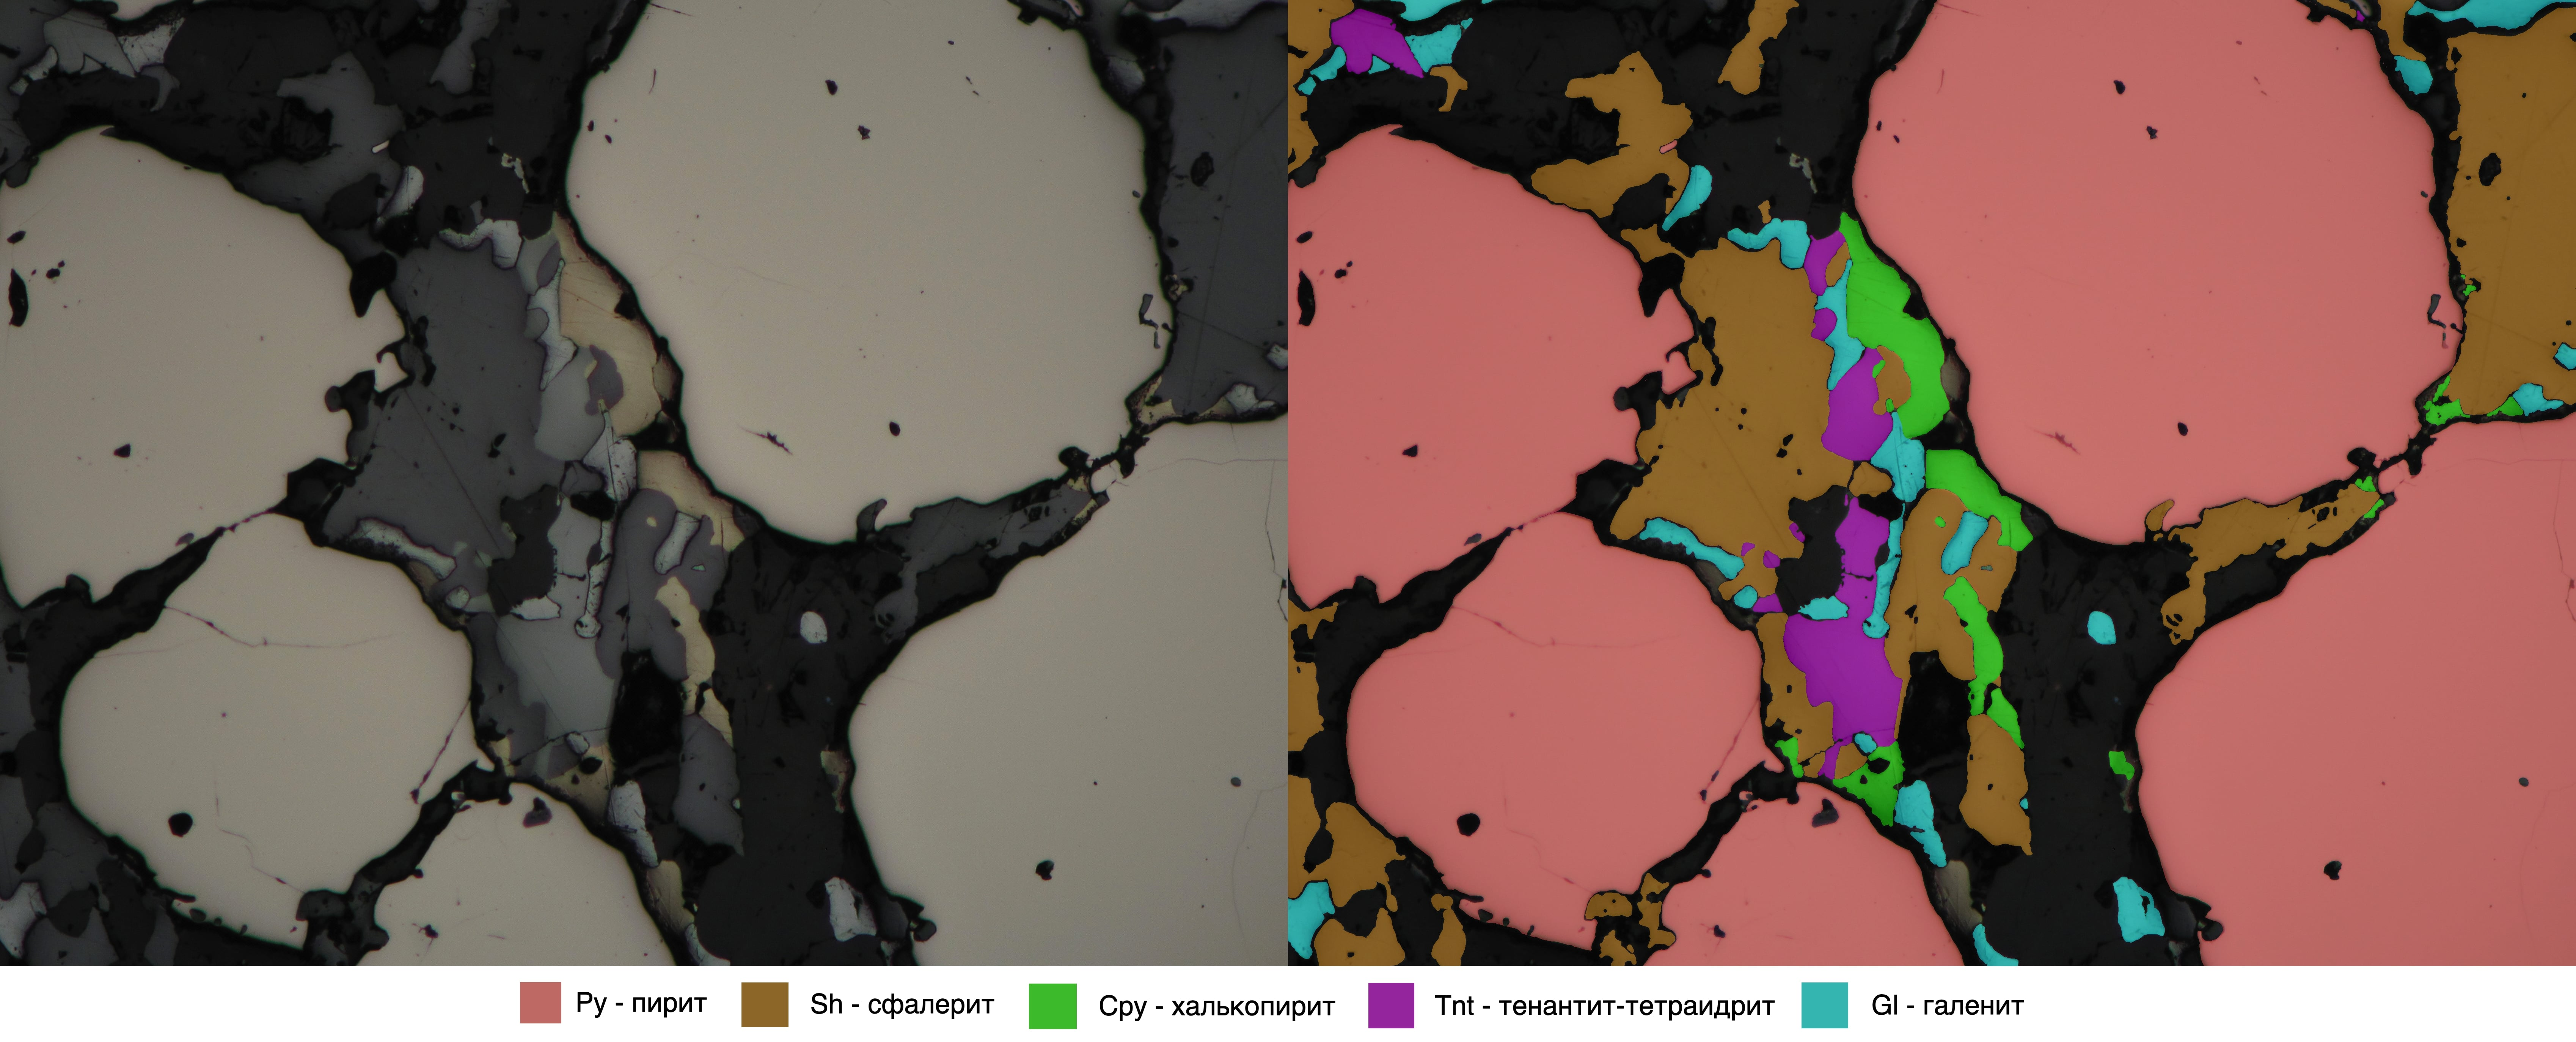
\includegraphics[width=\textwidth]{pics/segm_ex2.jpg}
    \centering
    \caption{Пример эталонной разметки изображения аншлифа.}
\end{figure}

\newpage
\section{Обзор существующих методов}
Семантическая сегментация - это процесс разбиения цифрового изображения на различные сегменты (наборы пикселей), включащий в себя
определение и изоляцию пикселей, принадлежащих к одному классу \cite{martinez2007petrographic}.
В анализе минералов обычно используется сегментация, основанная на выделении границ и областей, или всего вместе. \par
Существующие алгоритмы диагностики минералов основываются на статистическом анализе изображений.
\parВ \cite{berrezueta2016ore} описан следующий метод:
\begin{enumerate}[nosep]
    \item Вычисляются градации серого для каждого минерала на фотографии. Сверточные ядра размером $10\times 10$ накладываются на области, которые можно точно отнести к определенным минералам.
    \item Для минералов, изученных на предыдущем шаге вычисляются среднее $(x)$ и стандартное отклонение $(\sigma)$. Диапазоны сегментации определяются как $(x \pm \sigma)$, с уровнем заначимости $Y: 99.9\%$.
    \item Диапазоны сегментации для минерала 1 сохраняются в группе 1.
    \item Выбирается новый минерал (минерал 2) на изображении в группе 1 и шаги 1) - 3) повторяются, пока все минералы не будут обработаны в этой группе.
    \item Выбирается новое изображение (группа 2) и повторяются шаги 1-4.
\end{enumerate}
\par Установив диапазоны сегментации для каждого минерала на всех спектральных изображениях, окончательная сегментация получается как пересечение всех частичных сегментаций (применяя классификатор минимальной дистанции Махаланобиса). Предполагая нормальное распределение градаций серого ($Y(\mu -3\sigma < X < \mu +3\sigma):99.7\%$), окончательные результаты сегентации имеют уровень $Y: 98.7\%$.
\par Описанный выше метод основан на анализе изображений, полученных в результате мультиспектральной съемки \cite{catalina2009use, barnuevo2008ensayo}. Это позволяет получить большой объем информации и проводить глубокий анализ, однако такая съемка требует специализированного дорогостоящего оборудовния.
\par В \cite{kose2012statistical} описан похожий статистический метод, описание которого в виде алгоритма выглядит следующим образом:
\begin{enumerate}[nosep]
    \item Получение статистических свойств текущей области.
    \item Нормализация цветов в исходном изображении.
    \item Сегментация сыпучих и измельченных образцов.
    \item Применение статистической сегментации к пикселям, попавших в несколько классов в результате сегментации (при необходимости). 
    \item Применение метода увеличения области для дальнейшего улучшения используя предыдущие сегментированные пиксели (при необходимости).
    \item Заполнение кусочков, выпавших в результате шлифовки.
    \item Подсчет площади, размера, количества минералов и полостей на изображении. 
    \item Получение количественных и качественных значений для оценки результатов.
\end{enumerate}

\newpage
\section{Предлагаемый метод}
В данной выпускной квалификационной работе предлагается использовать метод сегментации изображений аншлифов, основанный на применении сверточных нейронных сетей и последующей обработкой результатов сегментации математическими методами обработки изображений. \par Несмотря на то, что методы глубокого обучения и, в частности, свёрточные нейронные сети приобретают все большую популярность,  примеров их использования в задачах анализа геологических изображений крайне мало, а имеющиеся примеры созданы с целью решения узких задач, таких как определение фазовых переходов вещества по снимкам XRF-микроанализатора, или определения количества органического компонента в шлифе \cite{osnkonstrmeh, disser1}. \par Нейросетевые модели отличаются хорошей обобщающей способностью, что вместе с применением современных математических методов обработки изображений делает их чрезвычайно полезным инструментом, который может быть использован для обработки и анализа геологических изображений, и позволяет рассчитывать на получение хороших результатов в решении поставленных задач.
\par В качестве нейросетевой модели для осуществления сегментации изображений в данной работе используется сверточная нейронная сеть U-Net \cite{ronneberger2015u}.
\newline
\begin{figure}[H]
    \centering
    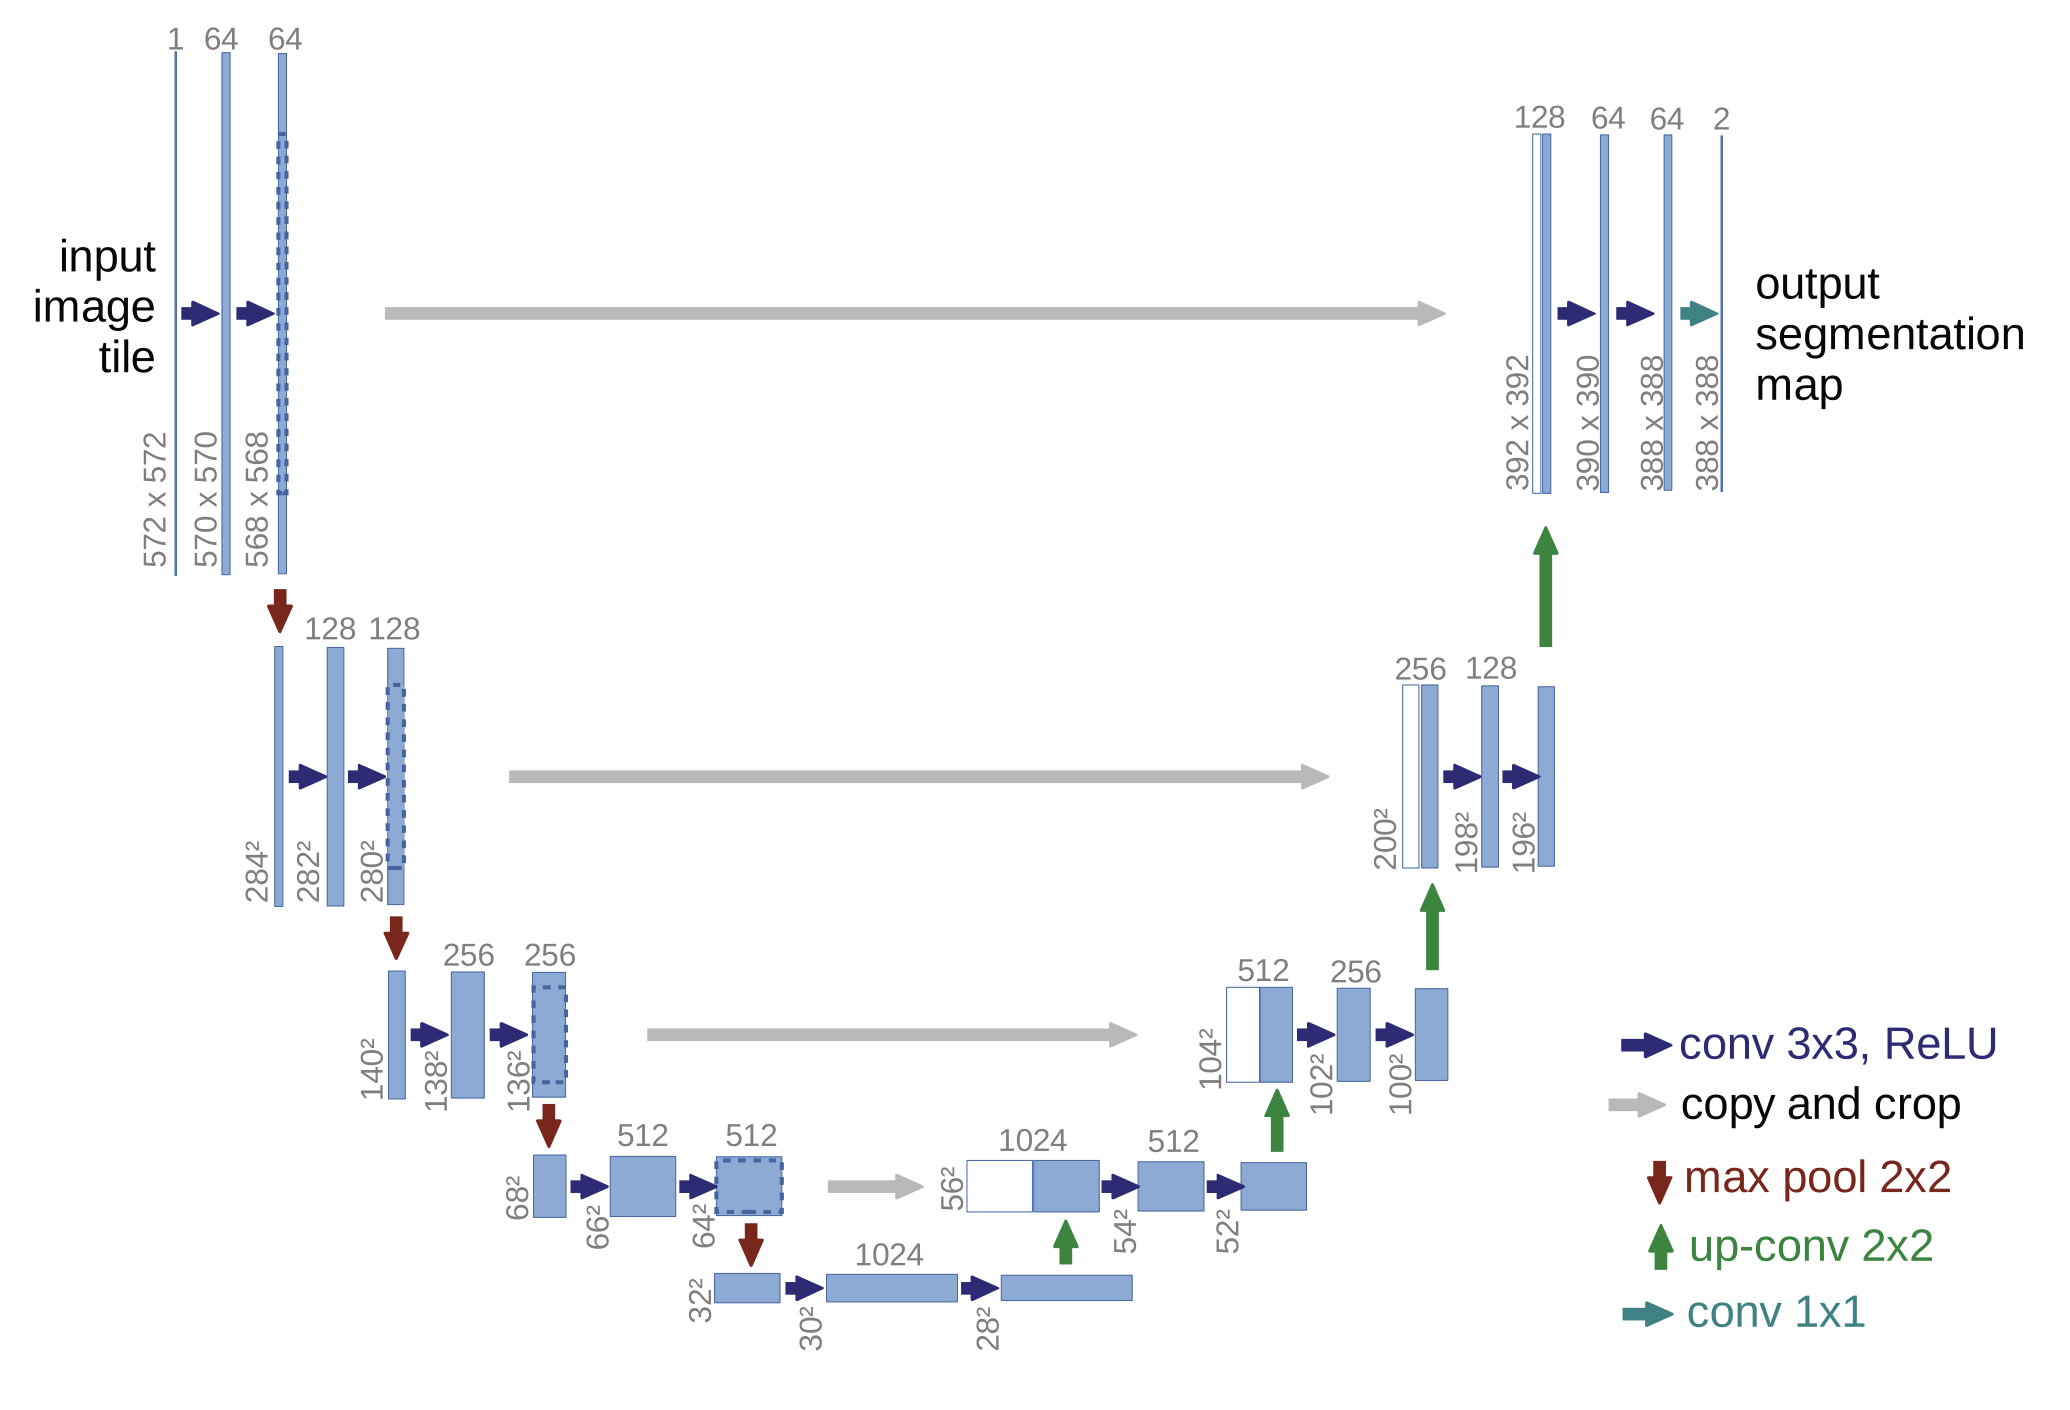
\includegraphics[width=0.75\textwidth]{pics/u-net.png}
    \caption{Архитектура сети U-Net. \textbf{Conv} - свертка, \textbf{max pool} - субдискретизация с выбором максимума, \textbf{up-conv} - транспонированая свертка.}
    % , \textbf{ReLU:} $f(x)=\begin{cases}
    % 0, & x<0 \\ x, & x \geqslant 0 \end{cases}$}
    \label{fig:unet}
\end{figure}
\newline
\par
Архитектура сети представляет собой полносвязную сверточную сеть, модифицированную так, чтобы она могла работать с меньшим количеством обучающих данных и делала более точную сегментацию. \par
Сеть содержит сжимающий путь (кодировщик) и расширяющий путь (декодировщик). Кодировщик состоит из сверточных блоков: две свертки с ядром $3 \times 3$, функцию активации $ReLu$ \footnote {$f(x)=\begin{cases} 0, & x<0 \\ x, & x \geqslant 0 \end{cases}$} и Max Pooling \footnote {слой субдискретизации с выбором максимума} $2 \times 2$ с шагом 2.
Декодировщик включает в себя блоки, состоящие из транспонированной свертки, свертки с ядром $2 \times 2$, конкатенации с соответствующим образом обрезанной карты признаков из кодировщика, затем идут две свертки с ядром $3 \times 3$ и функцией активации $ReLu$.  

\par Чем больше слоев используется в сети - тем выше обобщающая способность нейросети, тем самым качество сегментации повышается. С другой стороны, увеличение количества слоёв сети приводит к увеличению числа параметров, что требует больщего количества данных для обучения. На рисунке \ref{fig:unet} показана нейронная сеть с 4 слоями.

\newpage
\section{Проблема несбалансированности данных}
Используемые изображения аншлифов были сделаны по рудам свинцовоцинковых месторождений, относимых к колчеданному промышленному типу, который
связан с базальтовыми лавами. Все основные особенности месторождений и, в первую
очередь, состав руд (соотношения меди, цинка, свинца) обусловлены типом рудоносных
формаций. Среди основных минералов руд выделяются сфалерит (сульфид цинка),
халькопирит (сульфид меди), пирит (сульфид железа) и галенит (сульфид свинца). В
данном случае распределение металлов следующее: цинк – 60\%, медь – 30\%, свинец – 10\%.
Железо является вредной, не извлекаемой примесью и по этой причине не учитывается в
соотношении полезных ископаемых. Распространение рудных минералов соответствует
распределению металлов. Самый часто встречаемый минерал на изображениях – сфалерит,
менее распространённый пирит, за тем по встречаемости идёт халькопирит и наименее
распространённый минерал – галенит. 
\par В используемом наборе фотографий минерал галенит (\textbf{Gl}) пристутствует только на $6.7\%$ от общего числа пикселей. В то время как доля фона (\textbf{Background}), сфалерита (\textbf{Sh}), пирита и маркозита (\textbf{Py/Mrc}) составляет $33.7\%$, $29.3\%$ и $30.3\%$ соответственно.
\par
На вход нейронной сети подается квадратный фрагмент изображения (патч), который случайным образом вырезается из целого изображения. При случайном выборе патчей несбалансированность данных увеличивается. На тестовой выборке, состоящей из 1000 патчей, доля \textbf{Gl} составила менее $3\%$. Это приведет к тому, что распознавание этого минерала будет происходить гораздо хуже остальных ввиду недостатка данных на этапе обучения.
\par Таким образом, необходимо разработать и реализовать алгоритм, позволяющий решить проблему несбалансированности данных.
\newline
\newline
\newline
\par
Предлагается алгоритм, выполняющийся на каждом шаге эпохи обучения:
\begin{enumerate}[nosep]
    \item Определение класса, пиксели которого подавались в нейросеть наименьшее количество раз
    \item Выбор изображения, наиболее подходящего для текущего класса
    \item Выбор патча, содержащего наибольшее количество пикселей текущего класса
\end{enumerate}
\par Предложенный алгоритм балансировки будет работать одновременно с алгоритмом аугментации (искуственного расширения) данных. Для каждого патча будет происходить:
\begin{enumerate}[nosep]
    \item Поворот на произвольный угол
    \item Масштабирование с коэффициентом $\tau \in [\frac{1}{2}, 2]$
    \item Отражение по вертикали или горизонтали
    \item Поворот на 90 градусов по или против часовой стрелки
\end{enumerate}
Аугментация производится при недостатке данных и с целью предотвращения переобучения. \\
Рассмотрим алгорит балансировки подробнее.
\subsection{Определение класса}
Для поддержания сбалансированности количества пикселей каждого из классов изображения на этом шаге необходимо выбрать класс, число пикселей которого минимально среди всех пикселей, выбранных раньше.
Пусть имеется словарь, ключем которого является номер класса, а значением - число пикселей этого класса, которые уже были поданы на вход в нейросеть. Этот словарь обновляется по мере выбора патчей, а изначально все значения -- нули. Искомый класс -- это ключ, значение которого минимально в этом словаре.
\subsection{Выбор изображения}
После того, как стало известно, какой класс на данной итерации мы хотим выбирать, необходимо выбрать изображение, из которого будет вырезан патч. Для каждого из классов заранее был составлен словарь, ключом которого является \textbf{id} изображения, на котором данный класс присутствует. Значением является число пикселей, принадлежащих этому классу на изображении. 
\par
На каждом шаге необходимо выбирать $b$ патчей, где $b$ - размер пакета (batch size). Соответственно, необходимо выбрать $b$ изображений, в каждом из которых будет вырезан патч. Каждое изображение выбирается с вероятностью, равной числу пикселей класса на нем. Таким образом, на этом шаге мы получаем массив из $b$ элементов, каждый из которых является \textbf{id} изображения, на котором больше всего пикселей данного класса.
\subsection{Выбор патча}
После получения массива с \textbf{id} изображений, на каждом таком изображении необходимо выбрать патч, содержащий наибольшее число пикселей данного класса. Для этого необходимо построить для каждого из изображений карту вероятностей того, что верхний левый угол патча будет выбран в данном пикселе. Карта вероятностей строится для каждого класса отдельно. \par Алгоритм построения карты вероятностей будет состоять из следующих шагов:
\begin{enumerate}
    \item Построение карты расстояний до класса
    \item Построение интегрального изображения
    \item Построение карты вероятностей выбора патча
\end{enumerate}
%Рассмотрим алгоритм подробнее.
\subsubsection{Построение карты расстояний до класса}
Для построения карты вероятностей до класса воспользуемся преобразованием Distance transform \cite{fabbri20082d}.
Рассмотрим бинарное изображение $I(x,y)$. Оно может быть разделено на две части: объект (O - Object) и фон (B - Background).
$$
I(x, y) \in\{O, B\}
$$
Результатом преобразования является карта (изображение) $I_{d}(x,y)$, каждый пиксель которого содержит расстояние от этого пикселя до ближайшего пикселя объекта на изображении $I(x,y)$.
$$
I_{d}(x, y)=\left\{\begin{array}{ll}
0, & I(x, y) \in\{O\} \\
\min \left(\| x-x_{0}, y-y_{0} \|_{L_{2}}, \ \forall I\left(x_{0}, y_{0}\right) \in B \right), & I(x, y) \in\{B\}
\end{array}\right.
$$
$$
\|x, y\|_{L_{2}}=\sqrt{x^{2}+y^{2}}
$$
Рассмотрим на примере изображения $5 \times 5$.
$$
I = 
\begin{bmatrix}
 0&0&0&0&0 \\
 0&1&0&0&0 \\
 0&1&1&1&1 \\
 0&1&1&0&0 \\
 0&0&0&0&0
\end{bmatrix}
\quad
I_d=
\begin{bmatrix}
 \sqrt{2}&1&\sqrt{2}&2&2 \\
 1&0&1&1&1 \\
 1&0&0&0&0 \\
 1&0&0&1&1 \\
 \sqrt{2}&1&1&\sqrt{2}&2
\end{bmatrix}
$$

\subsubsection{Построение интегрального изображения}
Интегральным изображением \cite{bradley2007adaptive} (summed-up area table) называется изображение, каждый пиксель которого является суммой всех пикселей исходного изображения выше и левее текущего, включительно. Пусть $I(x, y)$ - исходное изображение. Тогда интегральным изображением для изображения $I(x, y)$ является
$$
I(x, y)=\sum_{x^{\prime} \leq x \atop y^{\prime} \leq y} i\left(x^{\prime}, y^{\prime}\right)
$$
Интегральное изображение позволяет быстро и эффективно посчитать сумму пикселей в любой прямоугольной области изображения, так как
$$
I_{int}(x, y)=I(x, y)+I_{int}(x, y-1)+I_{int}(x-1, y)-I_{int}(x-1, y-1)
$$
После того, как интегральное изображение было подсчитано, сумма значений в прямоугольнике $[x_0, x_1] \times [y_0, y_1]$ может быть подсчитана так:
$$
\sum_{x_{0}<x \leq x_{1} \atop y_{0}<y \leq y_{1}} i(x, y)=I(D)+I(A)-I(B)-I(C),
$$
где $A=(x_0, y_0),~B=(x_1, y_0),~C=(x_0, y_1),~D=(x_1, y_1).$
\newline
\begin{figure}[H]
    \centering
    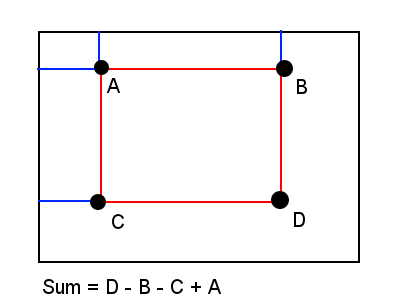
\includegraphics[width=0.5\textwidth]{pics/Summed_area_table.png}
    \caption{Вычисление суммы прямоугольной области при помощи интегрального изображения}
    \label{fig:summed0}
\end{figure}
\newpage
Рассмотрим вычисление суммы подробнее на примере изображения $6 \times 6$.
\newline
\begin{figure}[H]
    \centering
    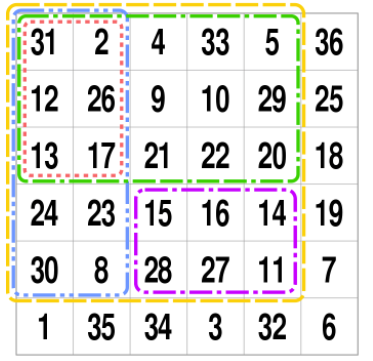
\includegraphics[width=0.25\textwidth]{pics/summedup1.png}
    \caption{Изначальное изображение. Вычисляется сумма значений элементов в фиолетовой области.}
    \label{fig:summed1}
\end{figure}
\begin{figure}[H]
    \centering
    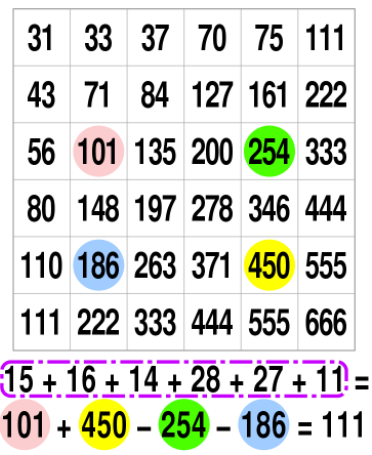
\includegraphics[width=0.25\textwidth]{pics/summedup2.png}
    \caption{Интегральное изображение. Вычисляется сумма значений элементов в фиолетовой области.}
    \label{fig:summed2}
\end{figure}

\subsubsection{Построение карты вероятностей выбора патча}
Применим к изображению $I(x,y)$ преобразование Distance transform ($I_{d}(x, y)$) и построим интегральное изображение от этого преобразования ($I_{int}(x,y)$). Рассмотрим на изображении квадратную область размера $p \times p$, где $p$ - ширина патча. Очевидно, что чем меньше сумма в соответствующей области на $I_{d}(x,y)$,
тем больше пикселей данного класса находится в соответствующей области изображения $I(x,y)$. 
\par Пусть $\tilde{I}_{d}(x,y) = 1 - \frac{I_{d}(x,y)}{max(I_{d}(x,y))}$, а соответствующее интегральное изображение обозначим $\tilde{I}_{int}(x,y)$. Получили, что чем \textit{больше} сумма в соответствующей области на $\tilde{I}_{d}(x,y)$, тем больше пикселей данного класса находится в соответствующей области изображения $I(x,y)$. Таким образом, при помощи $\tilde{I}_{int}(x,y)$ мы можем получить искомую карту вероятностей $P(x,y)$, в каждом пикселе которого содержится число, равное сумме расстояний от данного класса до фоновых пикселей. Очевидно, что чем значение в пикселе $P(x,y)$ выше, тем выше вероятность того, что при выборе патча с верхним левым углом в данном пикселе, на патч попадет наибольшее количество пикселей искомого класса. Таким образом, была получена карта вероятностей того, что левый верхний угол патча необходимо выбрать в данном пикселе с целью захватить наибольшее число пикслей данного класса.
\par Рассмотрим теперь данный алгоритм на примере изображения из обучающего набора. Предположим, что необходимо выбрать патч, содержащий наибольшее число пикселей, принадлежащих классу \textbf{Gl}, на изображении он размечен светло-зеленым цветом.
\newline
\begin{figure}[H]
    \centering
    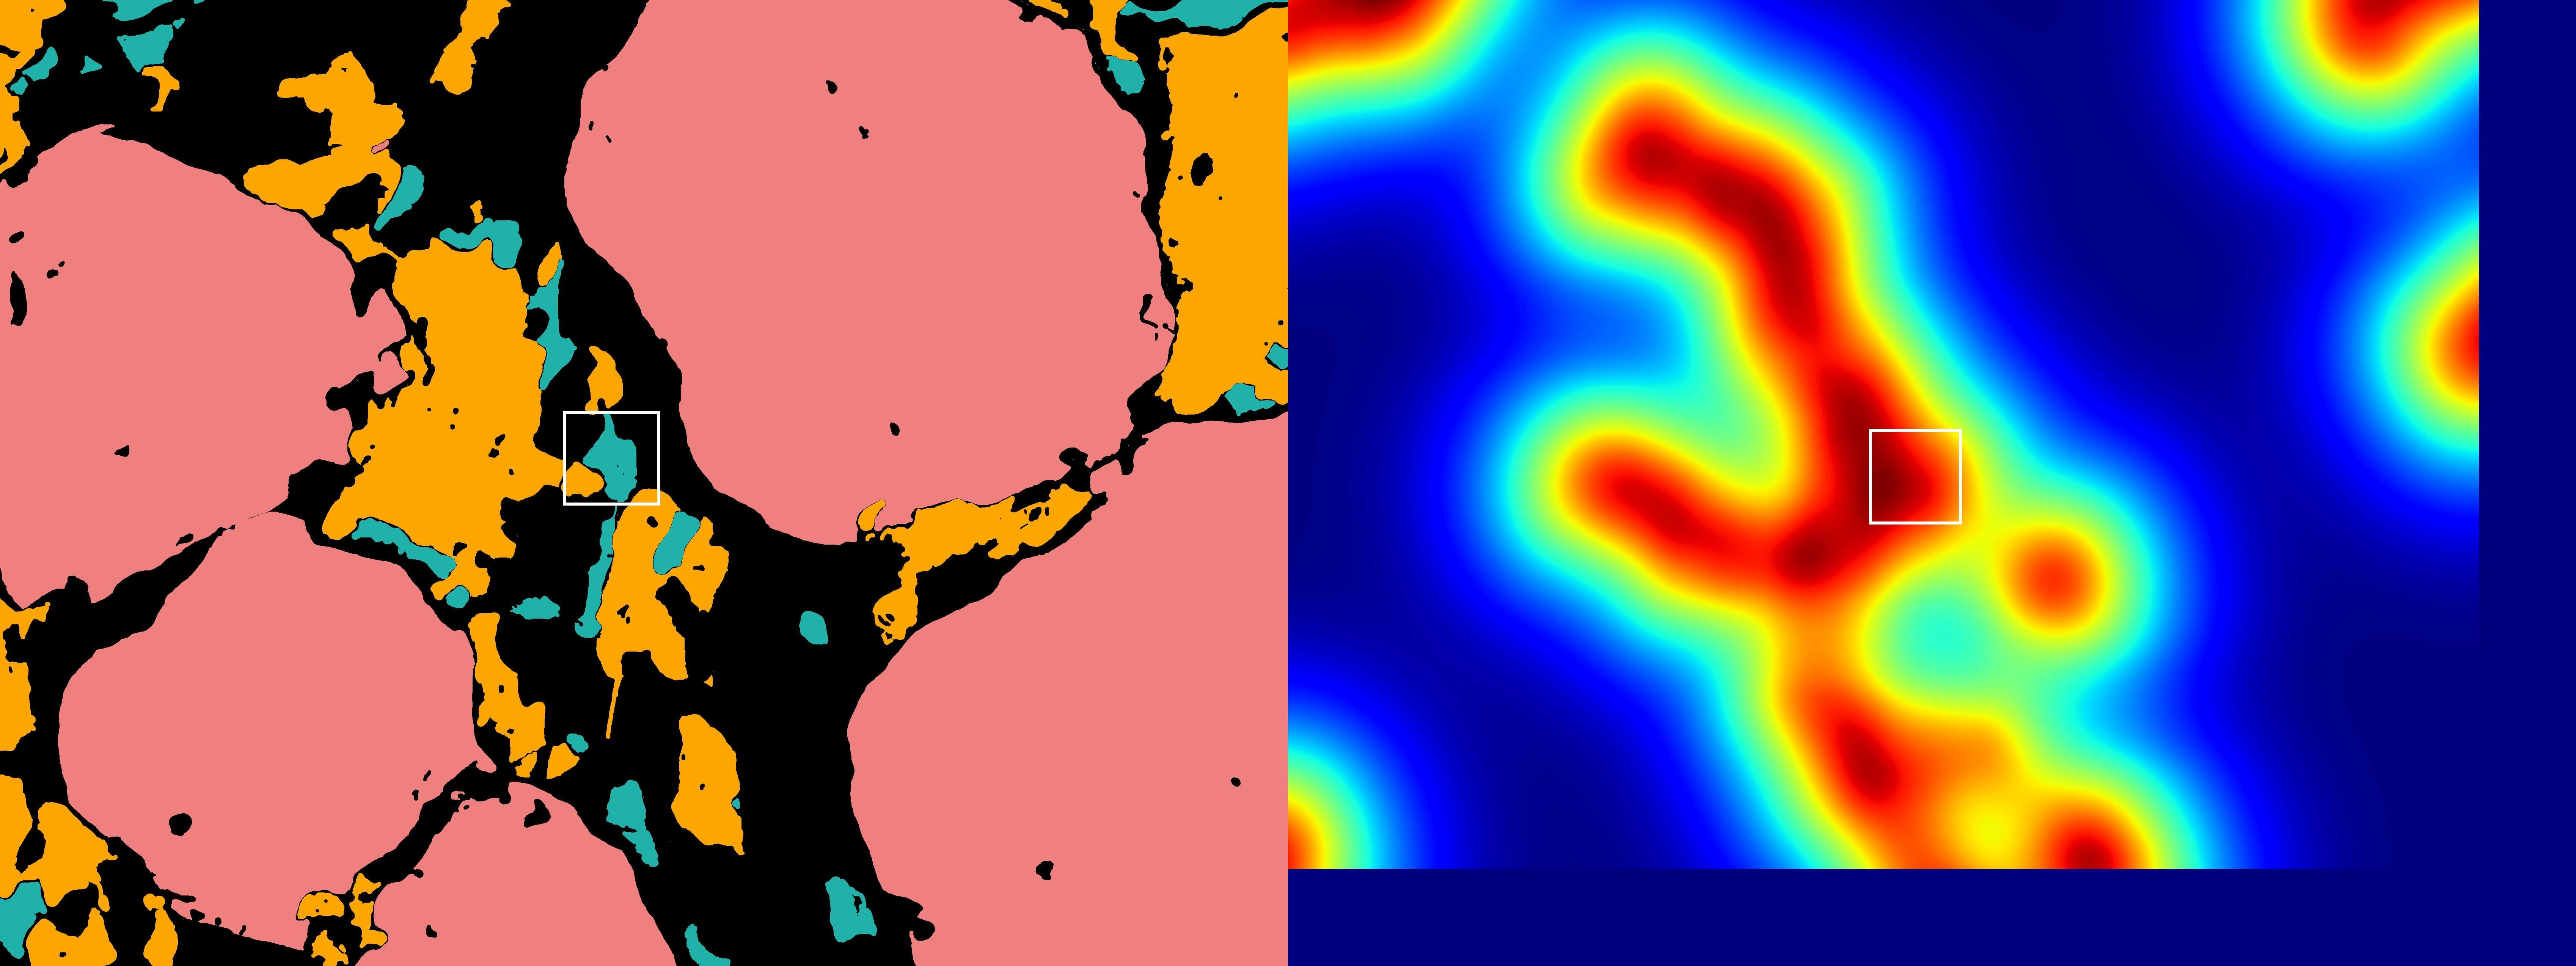
\includegraphics[width=0.95\textwidth]{pics/GL.jpg}
    \caption{Пример выбора патча. Слева - оригинальное изображение, справа - визуализация карты вероятностей.}
    \label{fig:algo}
\end{figure}
\par Красным цветом на карте вероятностей обозначены области, выбрав левый верхний угол патча в которых, мы получим наибольшее число пикселей нужного класса. Чем "холоднее" область, тем меньше вероятность попадания пикселей нужного класса на патч. "Холодные" полосы снизу и справа карты вероятностей, имеющие ширину, равную ширине патча, возникают из-за того, что в этой области нельзя выбрать выбрать патч, так как он выйдет за границы изображения.
\par Предложенный алгоритм балансировки данных позволяет добиться равного соотношения для каждого из классов. Это было проверено путем подсчета количества пикселей для каждого класса на большой выборке патчей (порядка 10000), полученных данным алгоритмом. Было получено следующее соотношение:
\begin{enumerate}[nosep]
    \item Background: 25.2\%
    \item Sh: 25.1\%
    \item Py/Mrc: 24.8\%
    \item Gl: 24.9\%
\end{enumerate}

\newpage
\section{Результаты сегментации}
Обучение нейронной сети было завершено по истечении 48 эпох, после того как значение функции потерь не уменьшалось в течение 4 эпох. Значение функции потерь составило $\approx 0.068$ (Рис. \ref{fig:train_loss}), а меры качества IoU $\approx 0.96$ (Рис. \ref{fig:train_iou}), что говорит о том, что нейронная сеть была хорошо обучена.
\\
\begin{figure}[H]
    \centering
    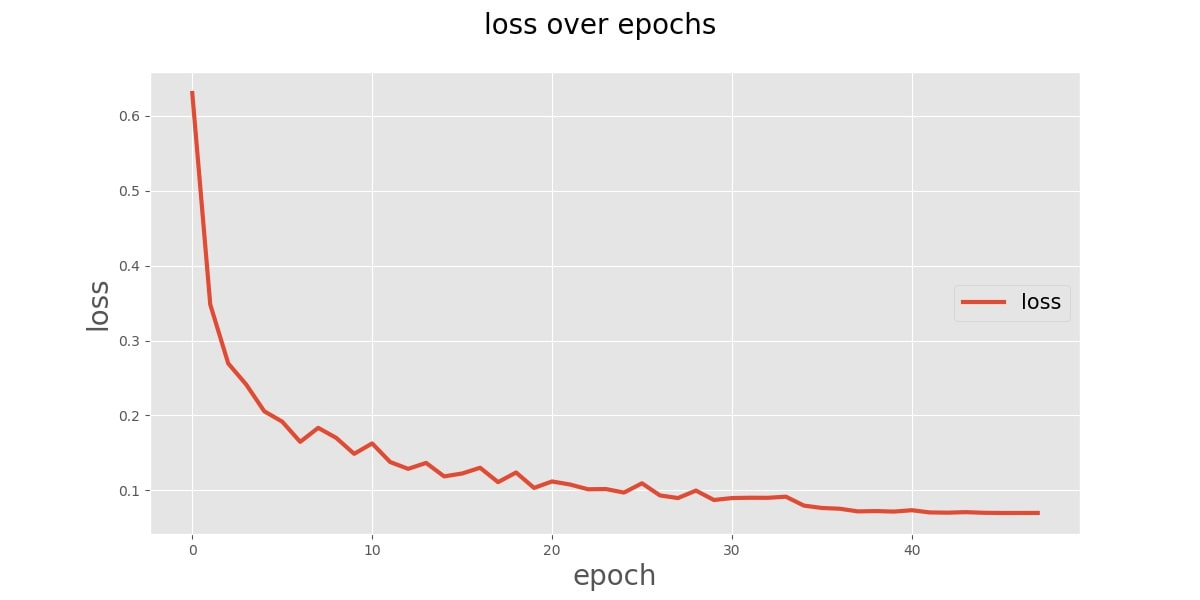
\includegraphics[width=0.95\textwidth]{pics/loss.jpg}
    \caption{Изменение значения функции потерь по эпохам обучения на тренировочных данных}
    \label{fig:train_loss}
\end{figure}

\begin{figure}[H]
    \centering
    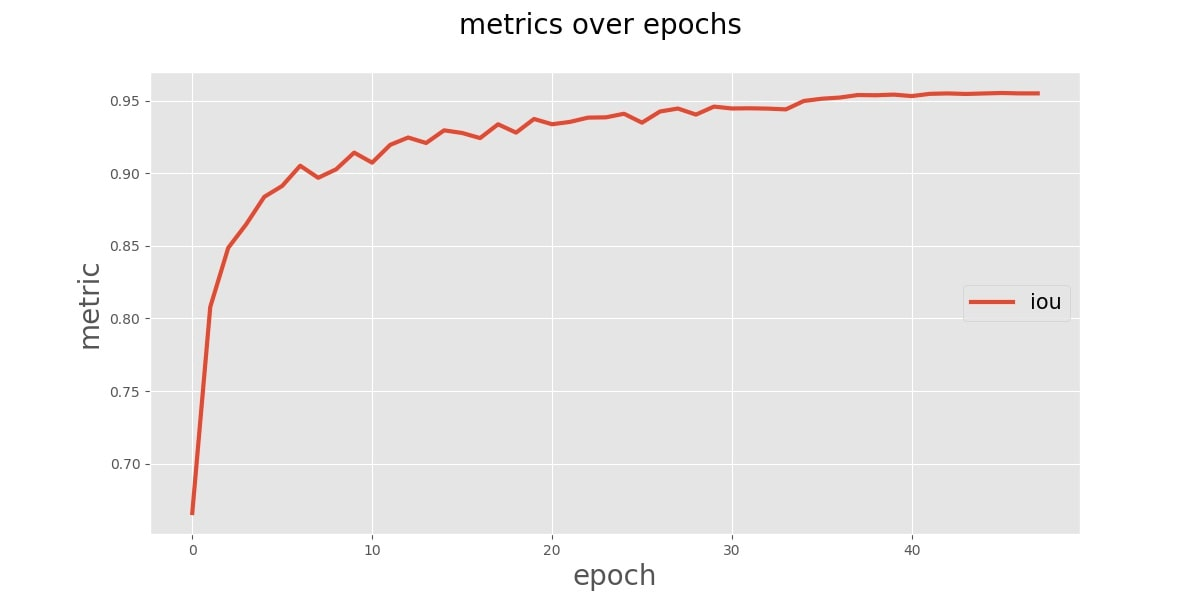
\includegraphics[width=0.95\textwidth]{pics/metrics.jpg}
    \caption{Изменение значения IoU по эпохам обучения на тренировочных данных}
    \label{fig:train_iou}
\end{figure}

После окончания каждой эпохи обучения нейронная сеть тестировалась на 11 изображениях, которые не подавались на вход во время обучения, то есть были не знакомы нейросети. Мера качества IoU показала следующие значения (в среднем по 11 изображениям):
\begin{itemize}
    \item Для каждого из классов (Рис. \ref{fig:test_iou}):
    \begin{enumerate}[nosep]
        \item Background: 0.82
        \item Sh: 0.78
        \item Py/Mrc: 0.95
        \item Gl: 0.57
    \end{enumerate}
    \item В среднем по всем классам (Рис. \ref{fig:test_iou_average}): 0.78
\end{itemize}
\begin{figure}[H]
    \centering
    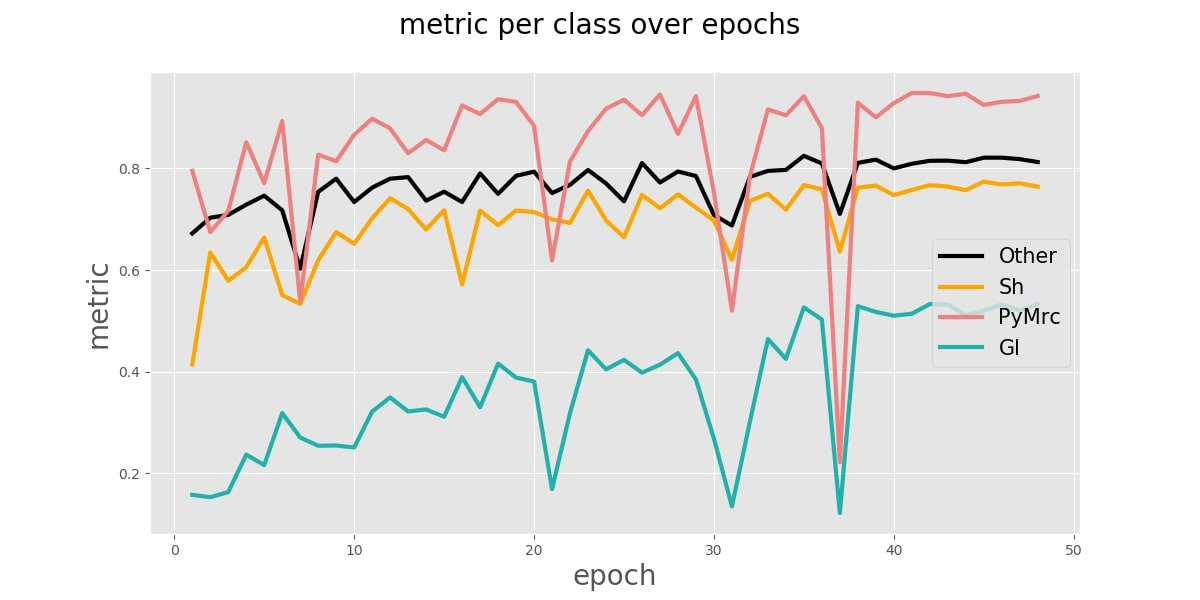
\includegraphics[width=0.95\textwidth]{pics/per_class_metric.jpg}
    \caption{Изменение значения IoU по эпохам обучения на тестовых данных для каждого класса}
    \label{fig:test_iou}
\end{figure}
\begin{figure}[H]
    \centering
    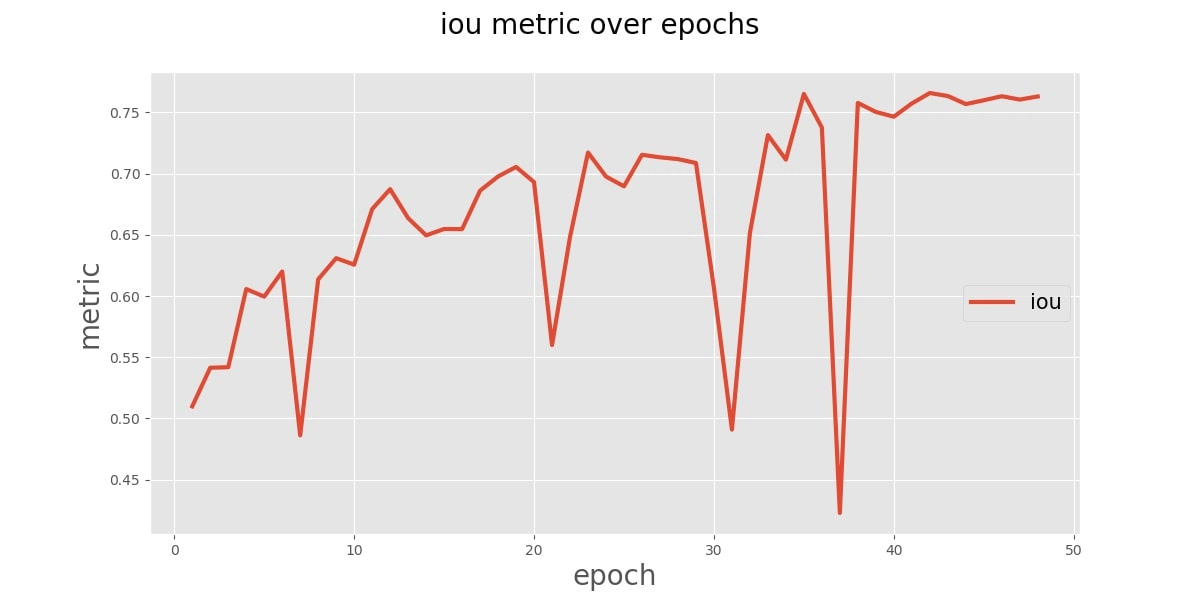
\includegraphics[width=0.95\textwidth]{pics/iou.jpg}
    \caption{Изменение значения IoU по эпохам обучения на тестовых данных}
    \label{fig:test_iou_average}
\end{figure}
\newpage
Далее приведены некоторые из тестовых изображений. Для каждого из изображений представлено:
\begin{enumerate}
    \item Исходное изображение -- фотография аншлифа
    \item Экспертная разметка -- выполненная вручную эталонная разметка минералов
    \item Предсказание -- результат работы алгоритма сегментации минералов
    \item Карта ошибок -- бинарная маска, в которой красным цветом обозначены области изображения, распознанные неправильно (там, где различаются предсказание и экспертная разметка), правильно распознанные области обозначены зеленым цветом
    \item Карта ошибок + исходное изображение -- наложение карты ошибок на изображение с фотографией аншлифа, позволяющее определить области изображения, которые не удалось распознать
\end{enumerate}{}
\par Также для каждого из изображений приведен процент правильной распознаваемости, показывающий насколько предсказание совпадает с экспертной разметкой.
\newpage

\begin{figure}[H]
\begin{subfigure}{.33\textwidth}
  \centering
  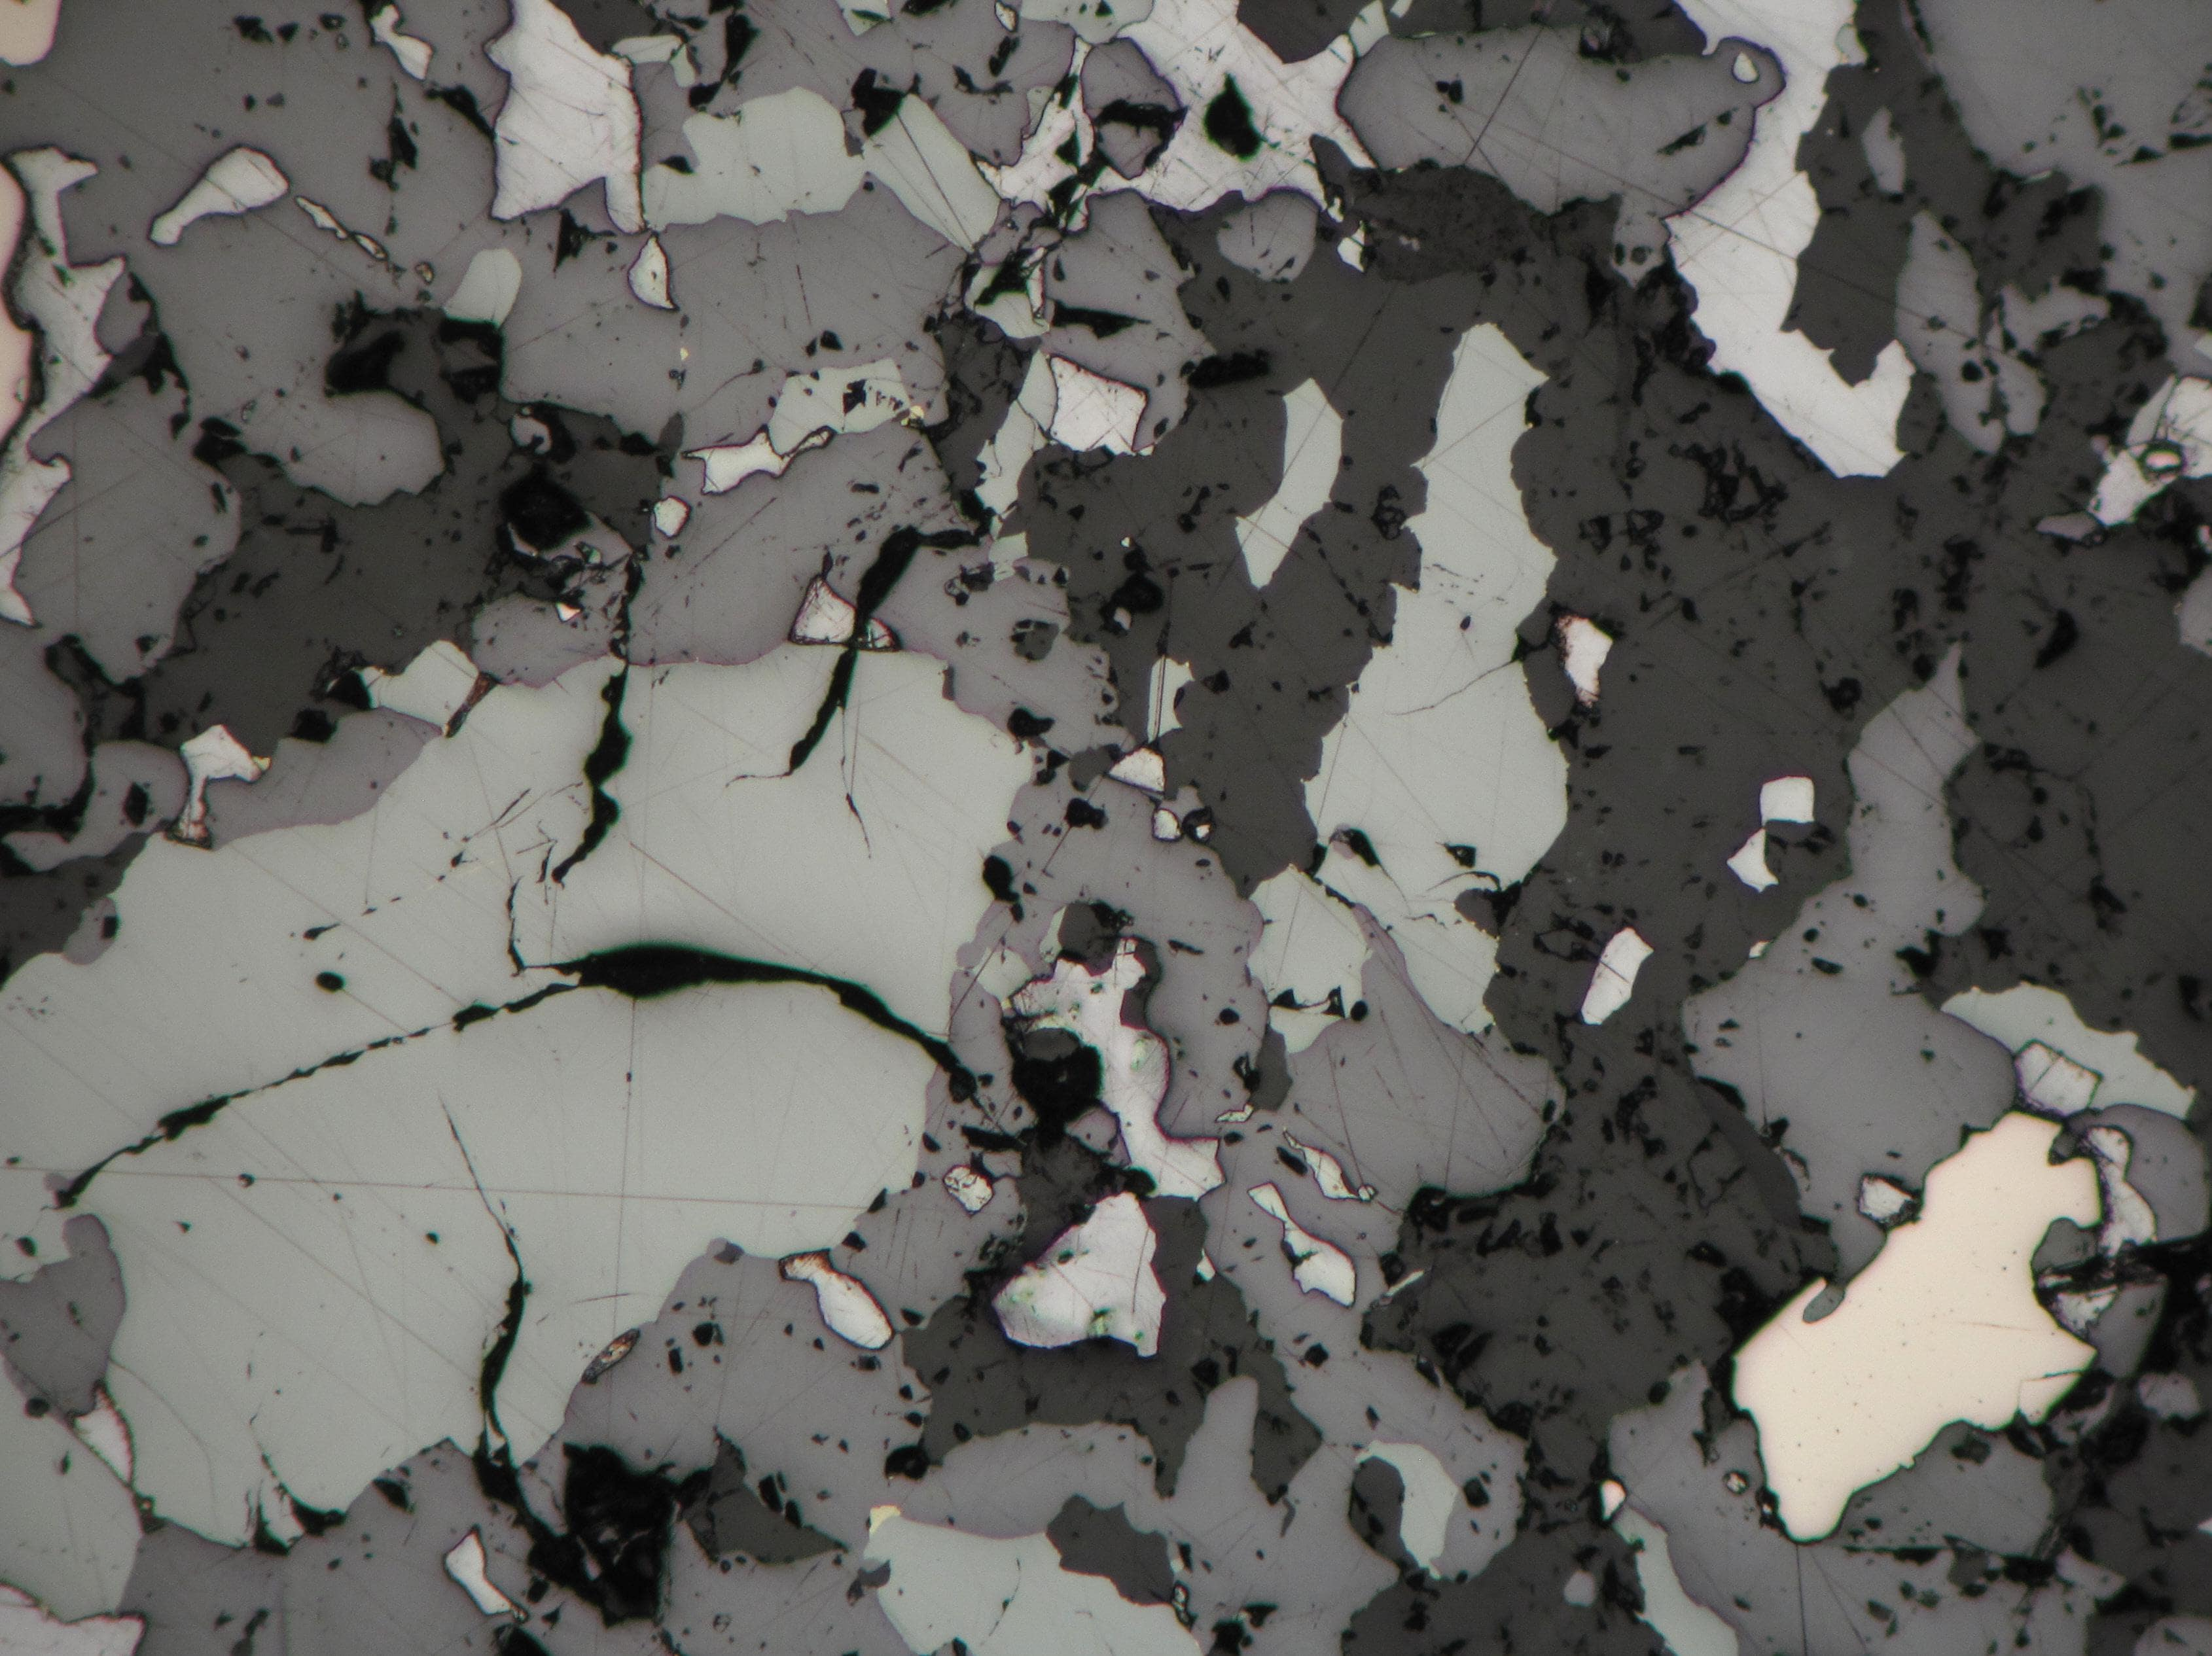
\includegraphics[width=.9\linewidth]{pics/image_3_src.jpg}
  \caption{Исходное изображение}
  \label{fig:sfig1_1}
\end{subfigure}%
\begin{subfigure}{.33\textwidth}
  \centering
  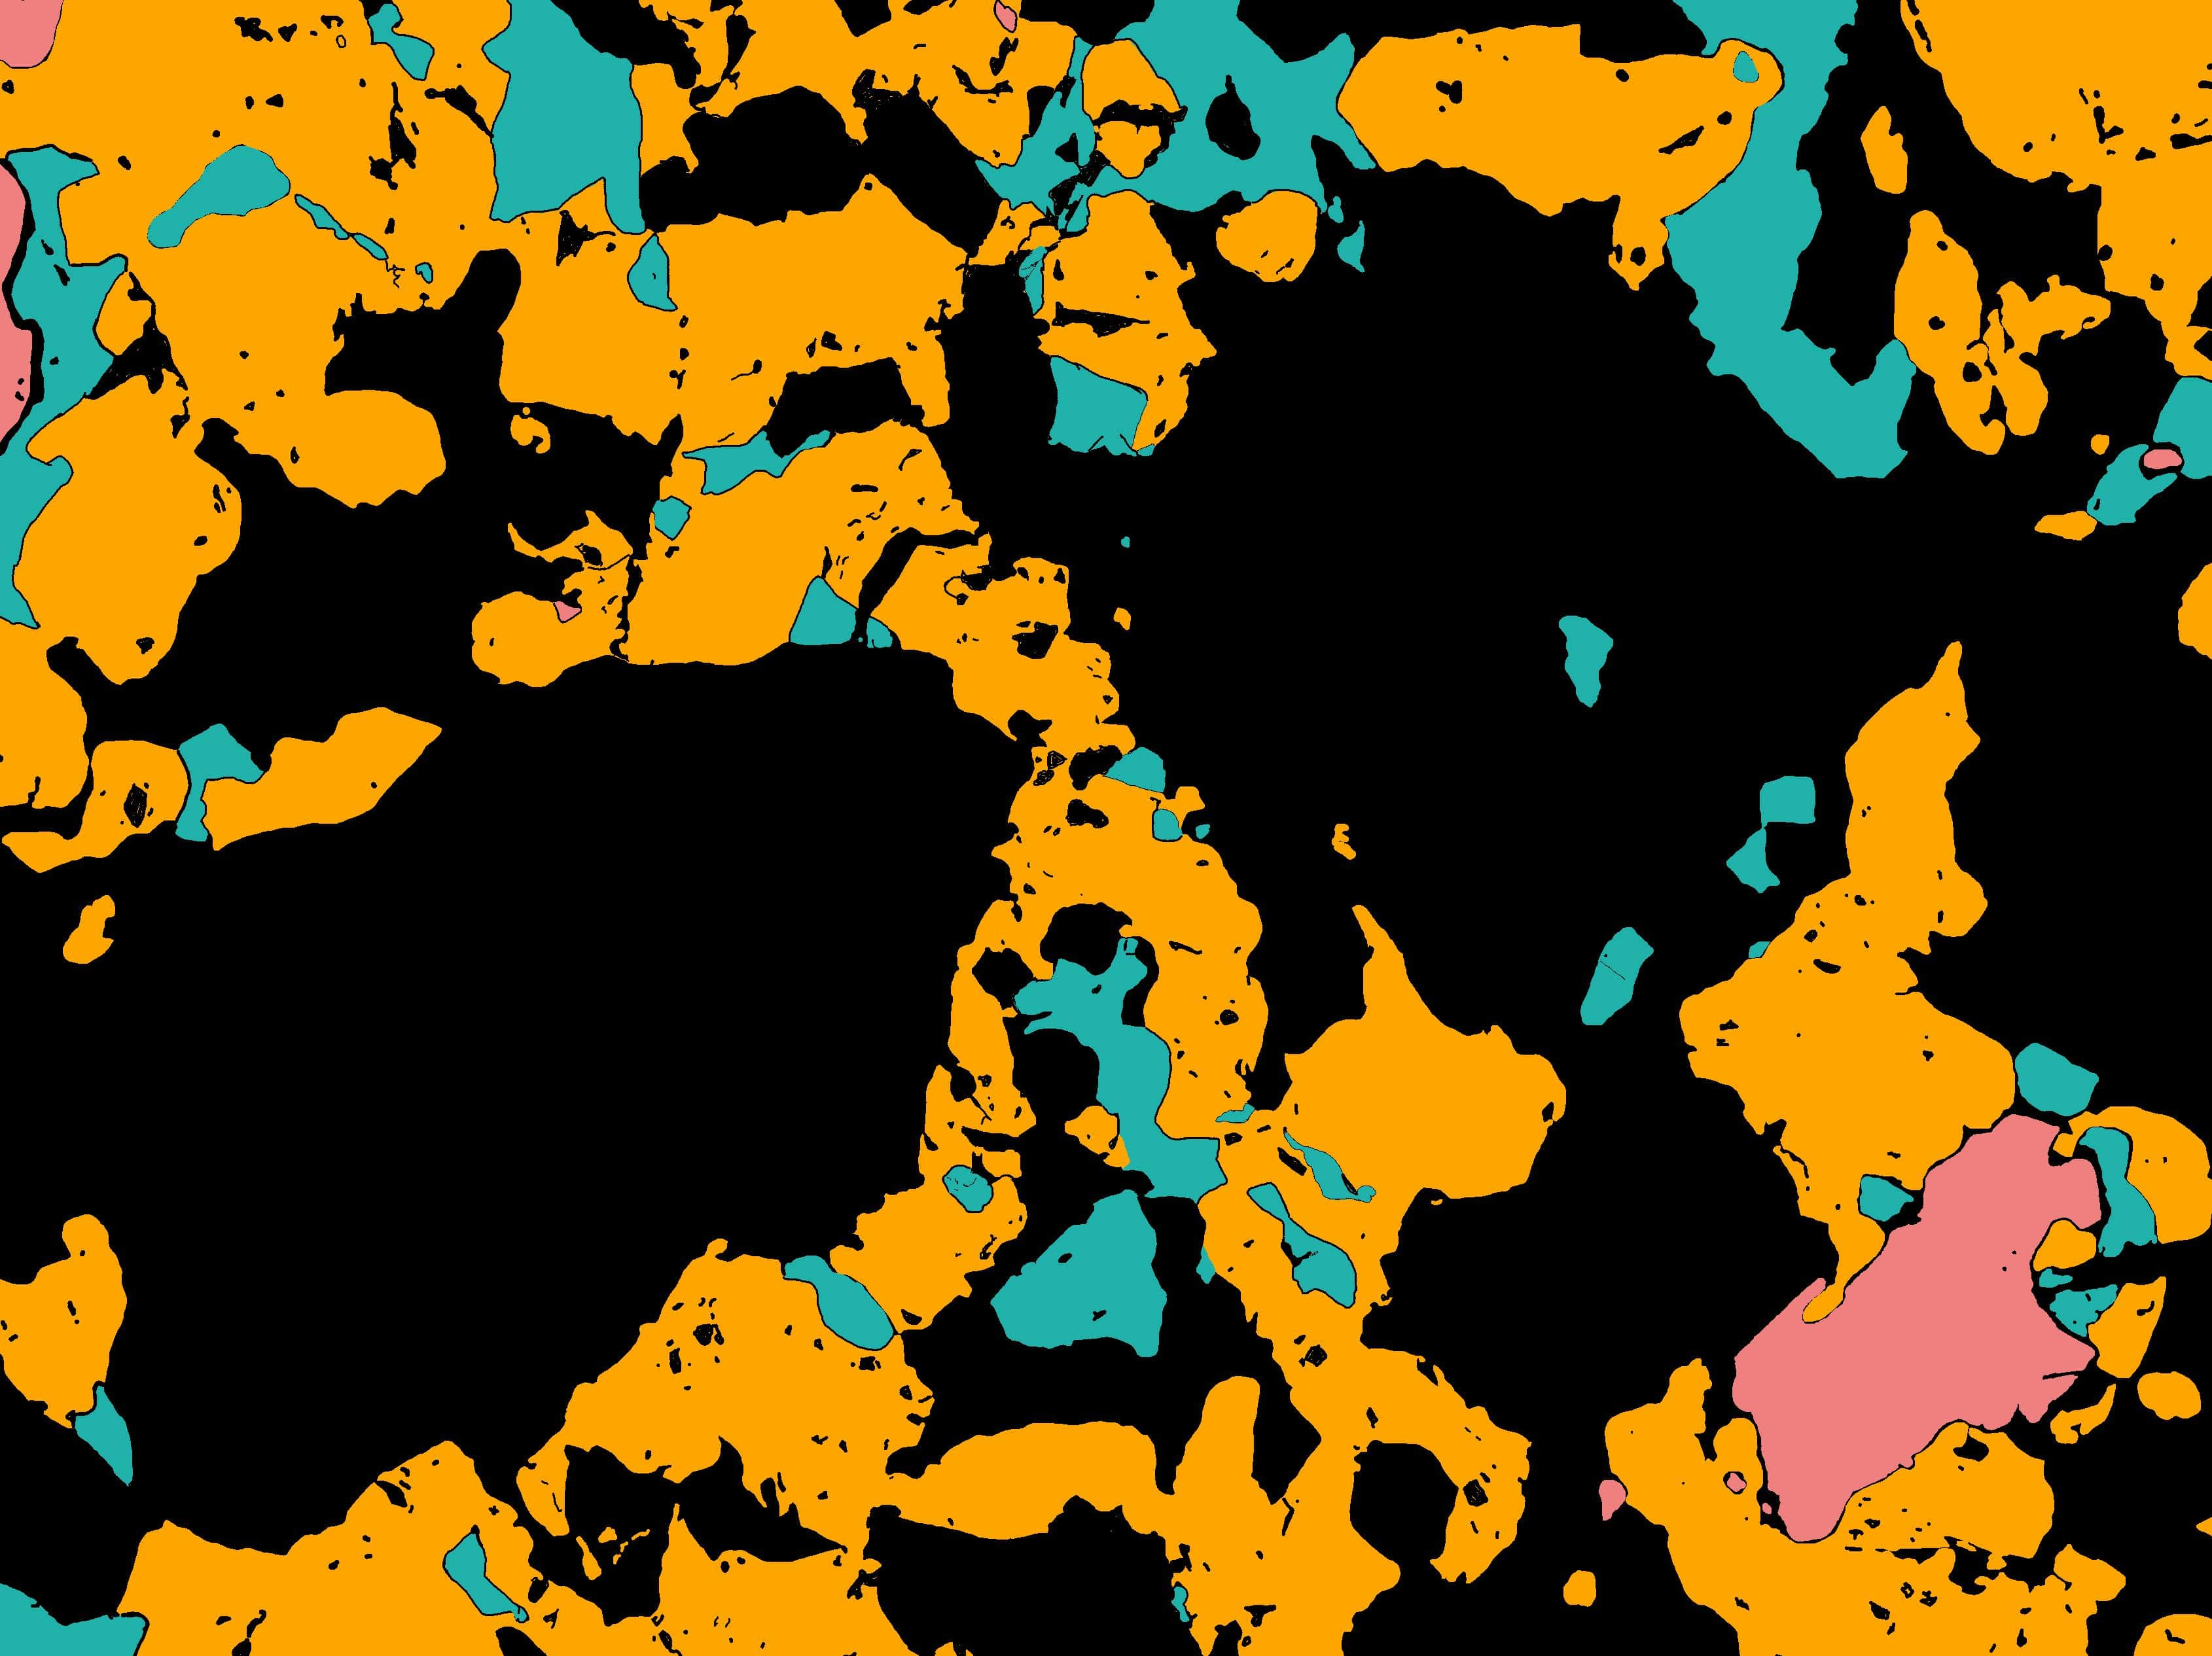
\includegraphics[width=.9\linewidth]{pics/image_3_gt.jpg}
  \caption{Экспертная разметка}
  \label{fig:sfig1_2}
\end{subfigure}%
\begin{subfigure}{.33\textwidth}
  \centering
  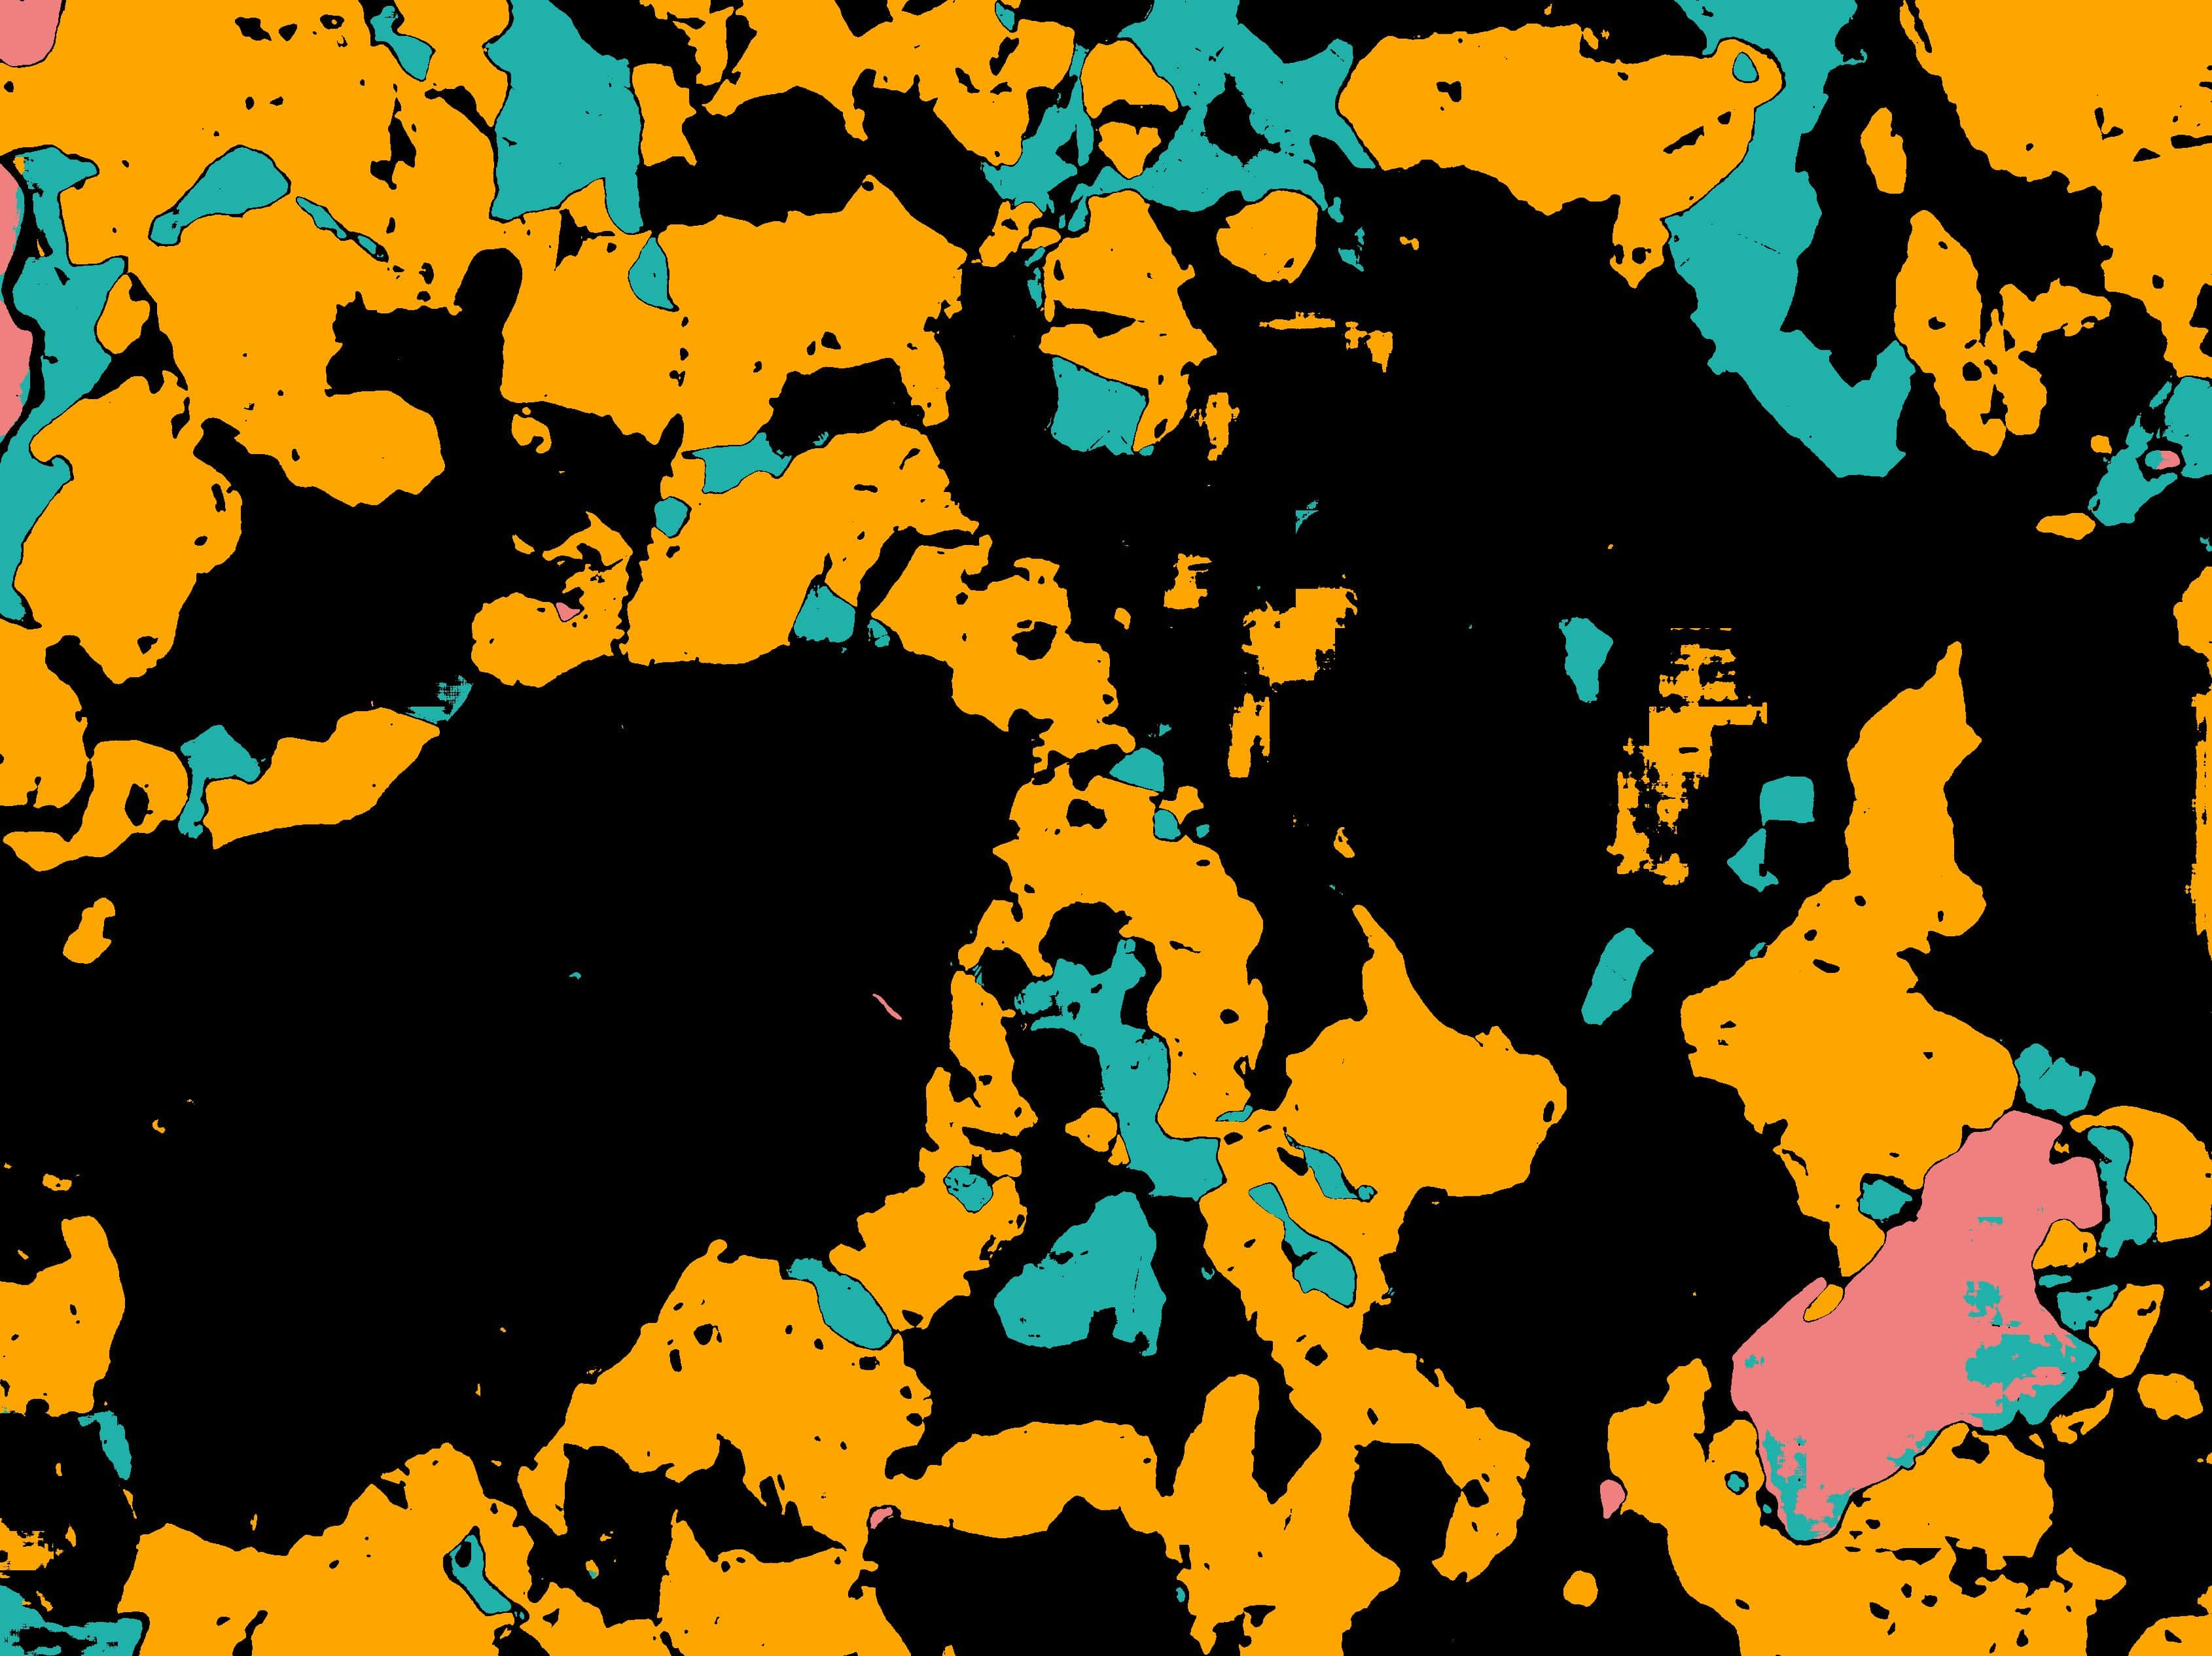
\includegraphics[width=.9\linewidth]{pics/image_3_pred.jpg}
  \caption{Предсказание}
  \label{fig:sfig1_3}
\end{subfigure} \\
\centering
\begin{subfigure}{.33\textwidth}
  \centering
  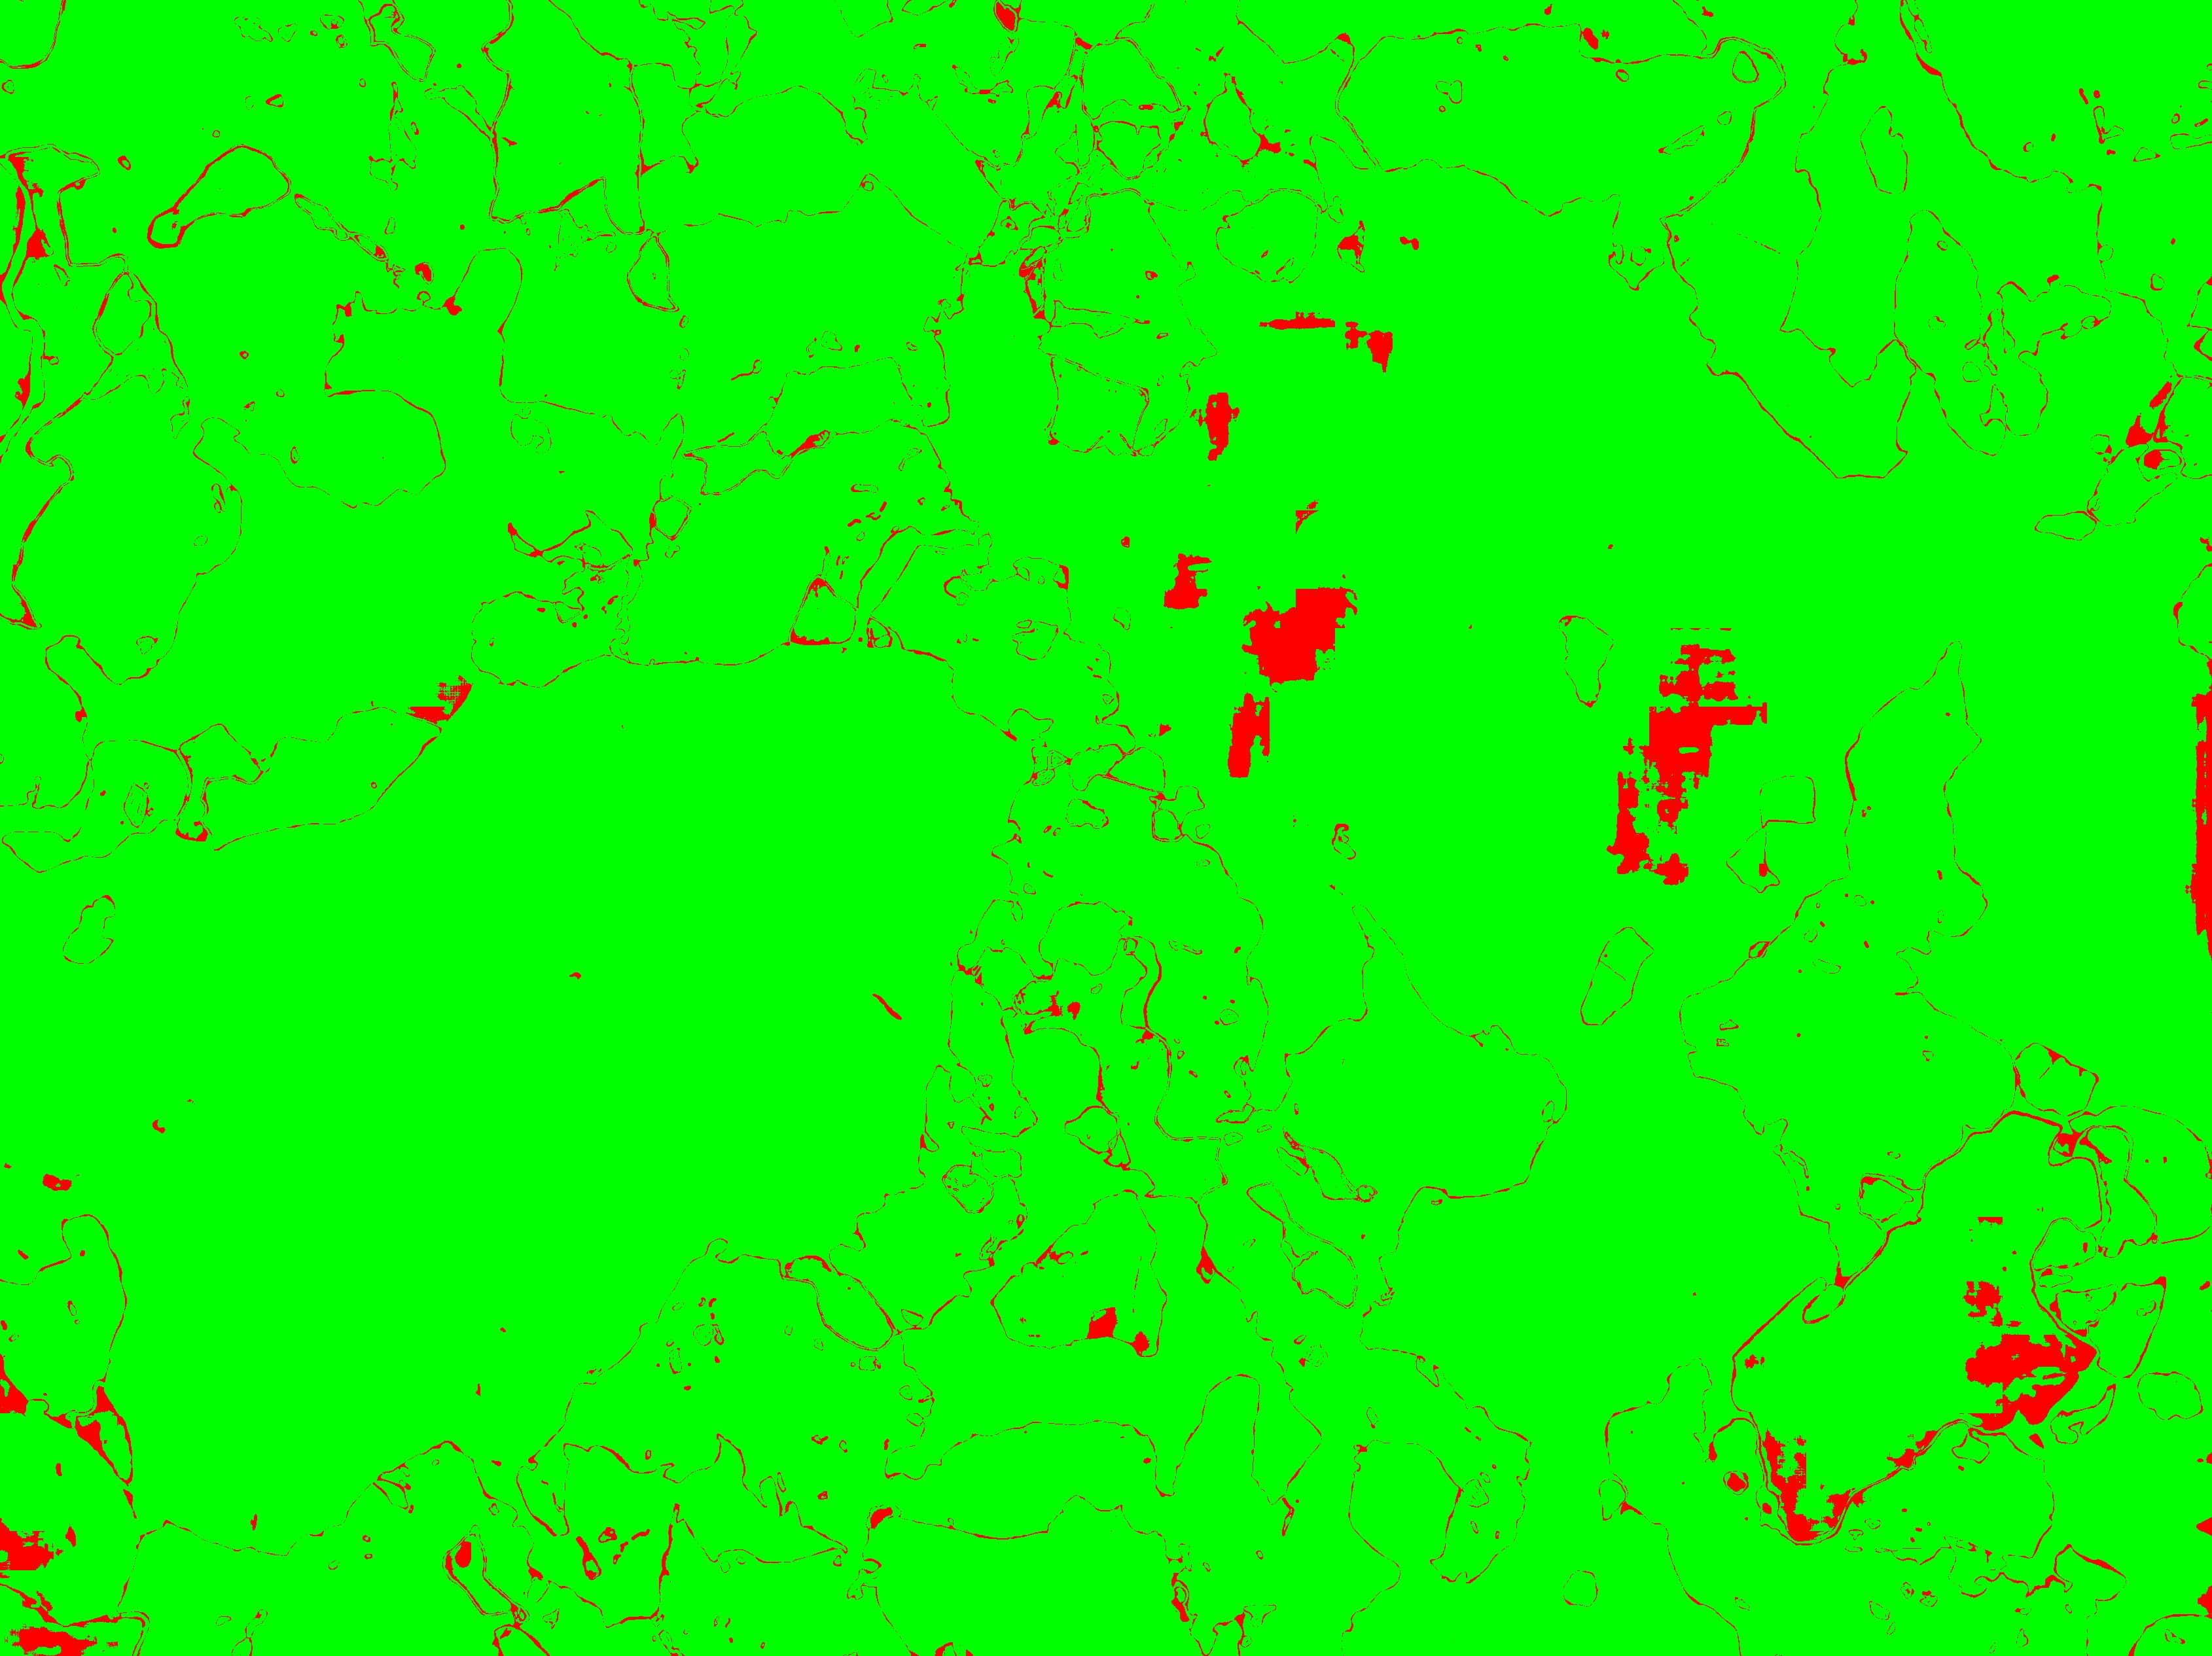
\includegraphics[width=.9\linewidth]{pics/image_3_error.jpg}
  \caption{Карта ошибок}
  \label{fig:sfig1_4}
\end{subfigure}%
\begin{subfigure}{.33\textwidth}
  \centering
  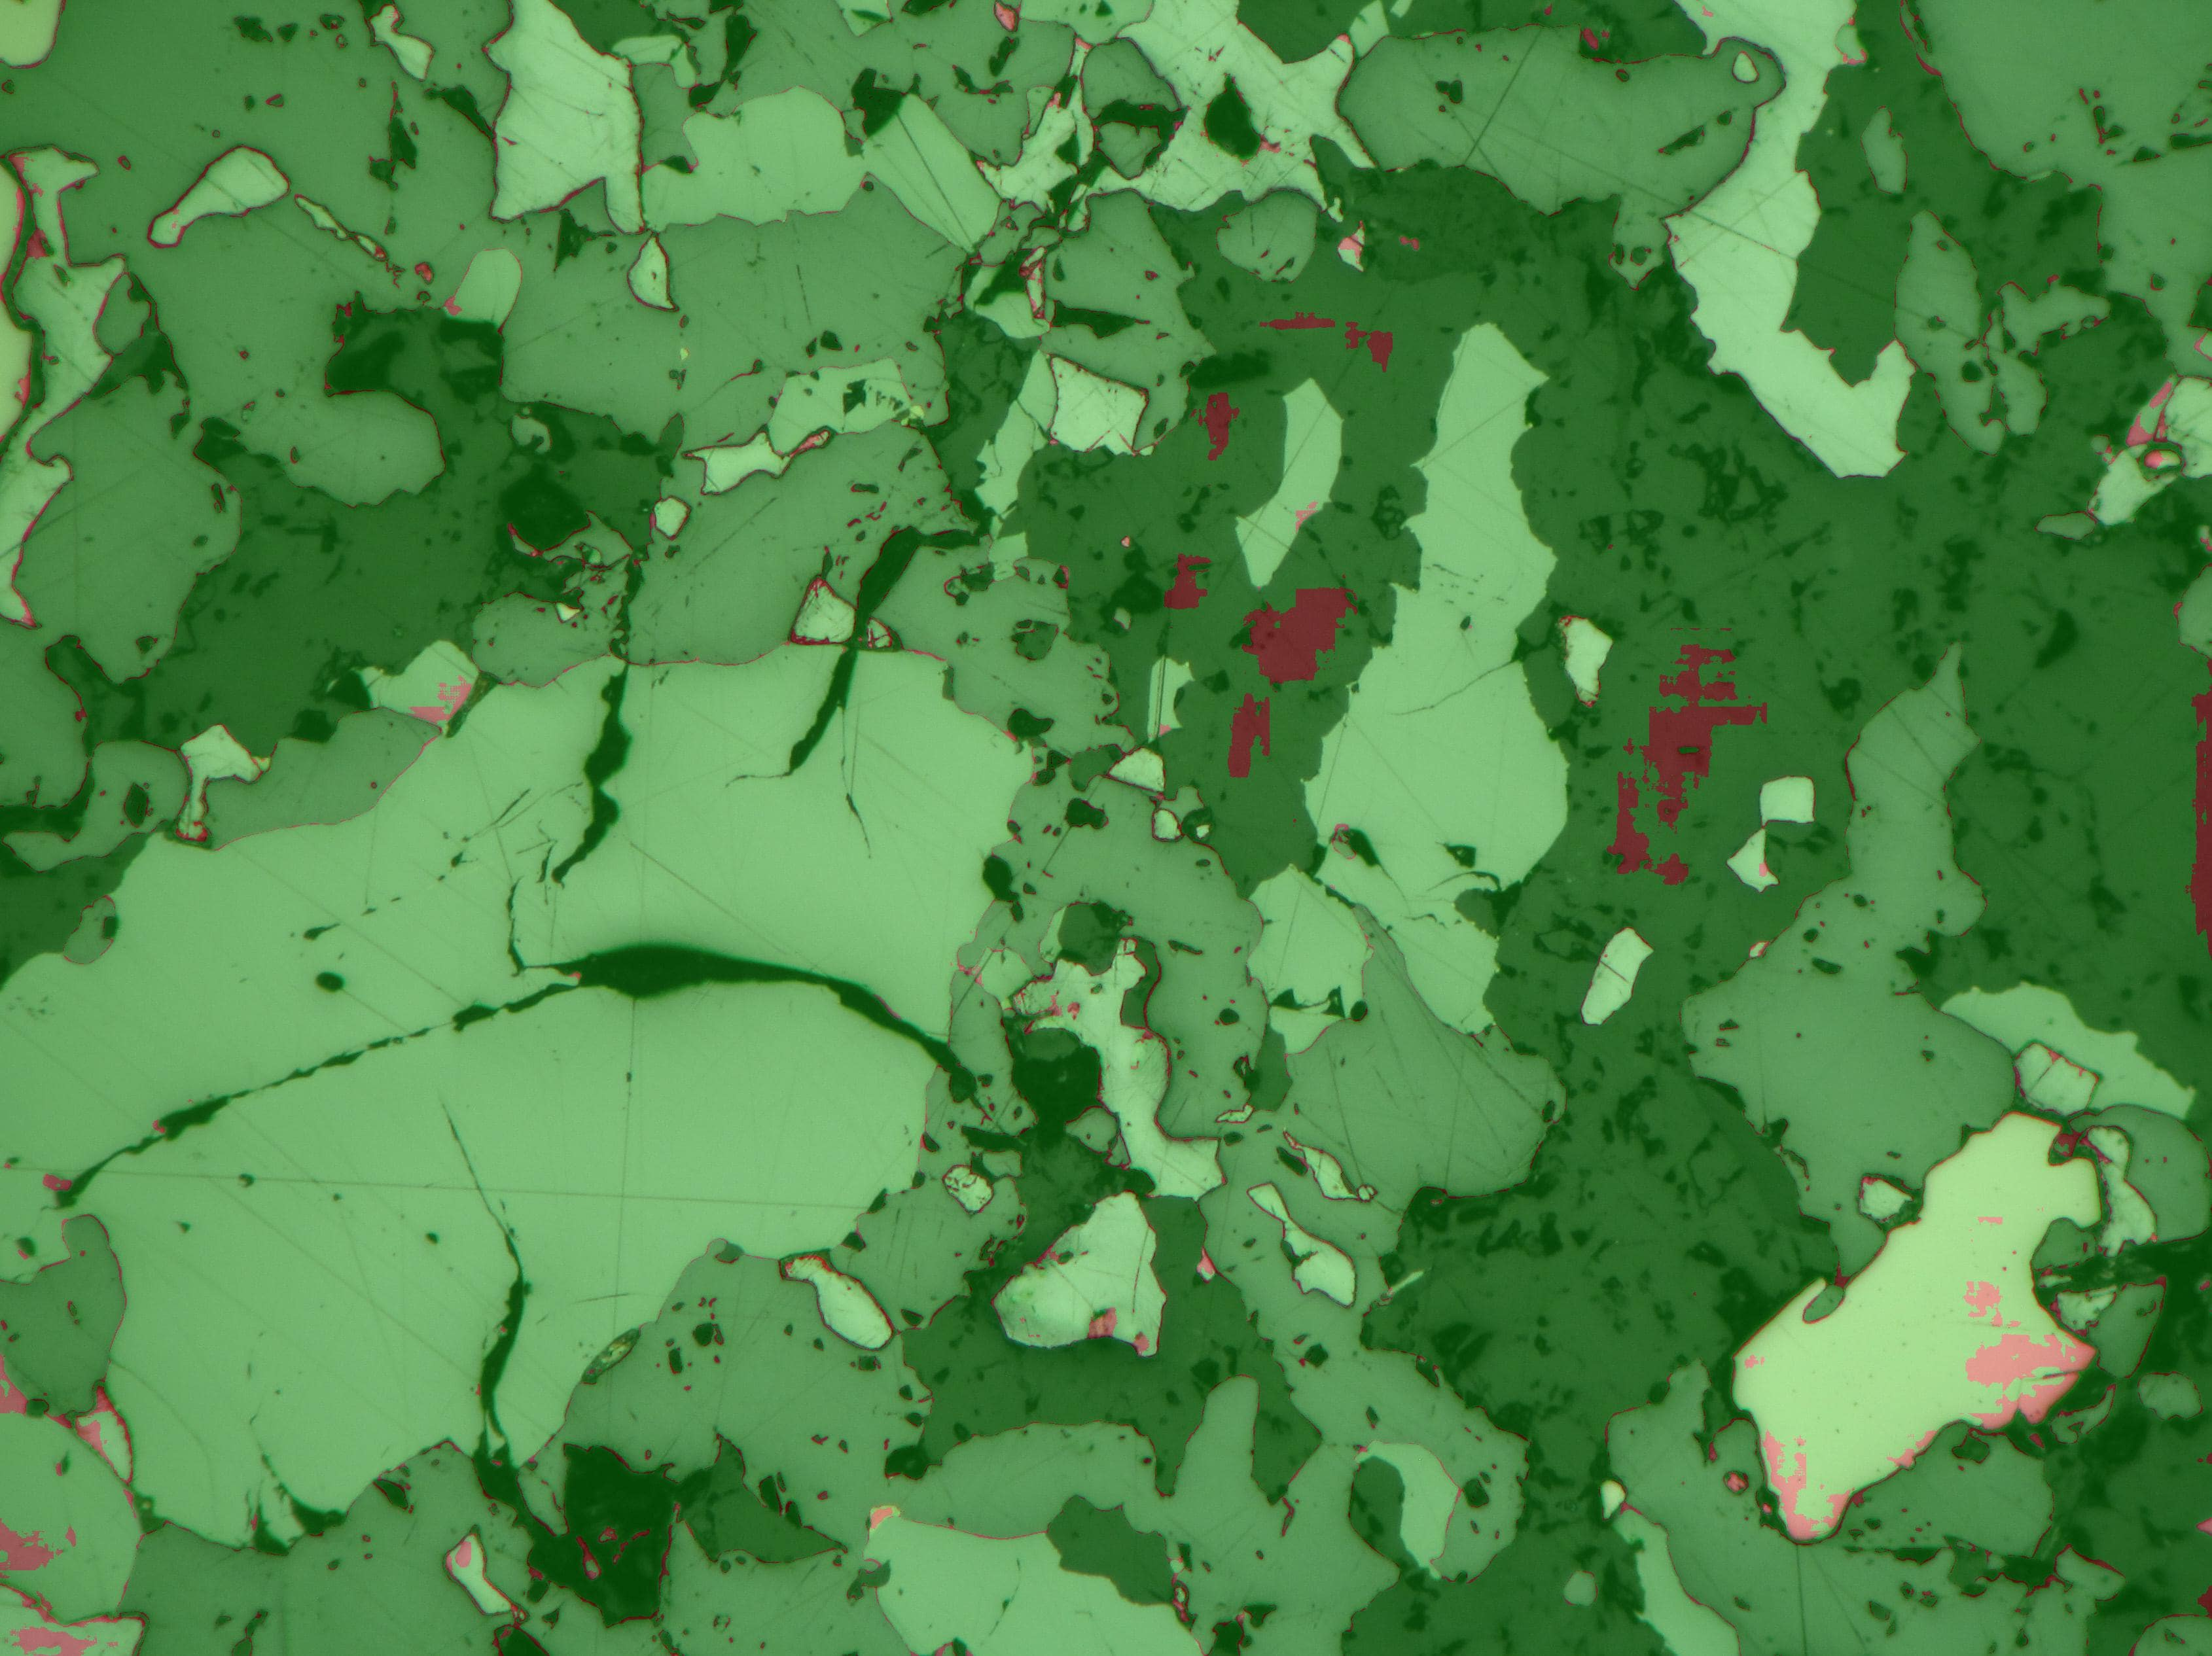
\includegraphics[width=.9\linewidth]{pics/image_3_overlay.jpg}
  \caption{Карта ошибок + исходное}
  \label{fig:sfig1_5}
\end{subfigure}
\caption{Тестовое изображение №1}
\label{fig:pred1}
\end{figure}
Тестовое изображение №1 было распознано правильно на 96.574\%, каждый из классов был распознан: \\
\begin{enumerate}[nosep]
    \item Background: 97.297\%
    \item Sh: 97.335\%
    \item Py/Mrc: 85.927\%
    \item Gl: 90.861\%
\end{enumerate}{}
Мера качества IoU показала следующие результаты:
\begin{enumerate}[nosep]
    \item Background: 0.93
    \item Sh: 0.92
    \item Py/Mrc: 0.8
    \item Gl: 0.81
\end{enumerate}{}

\begin{figure}[H]
\begin{subfigure}{.33\textwidth}
  \centering
  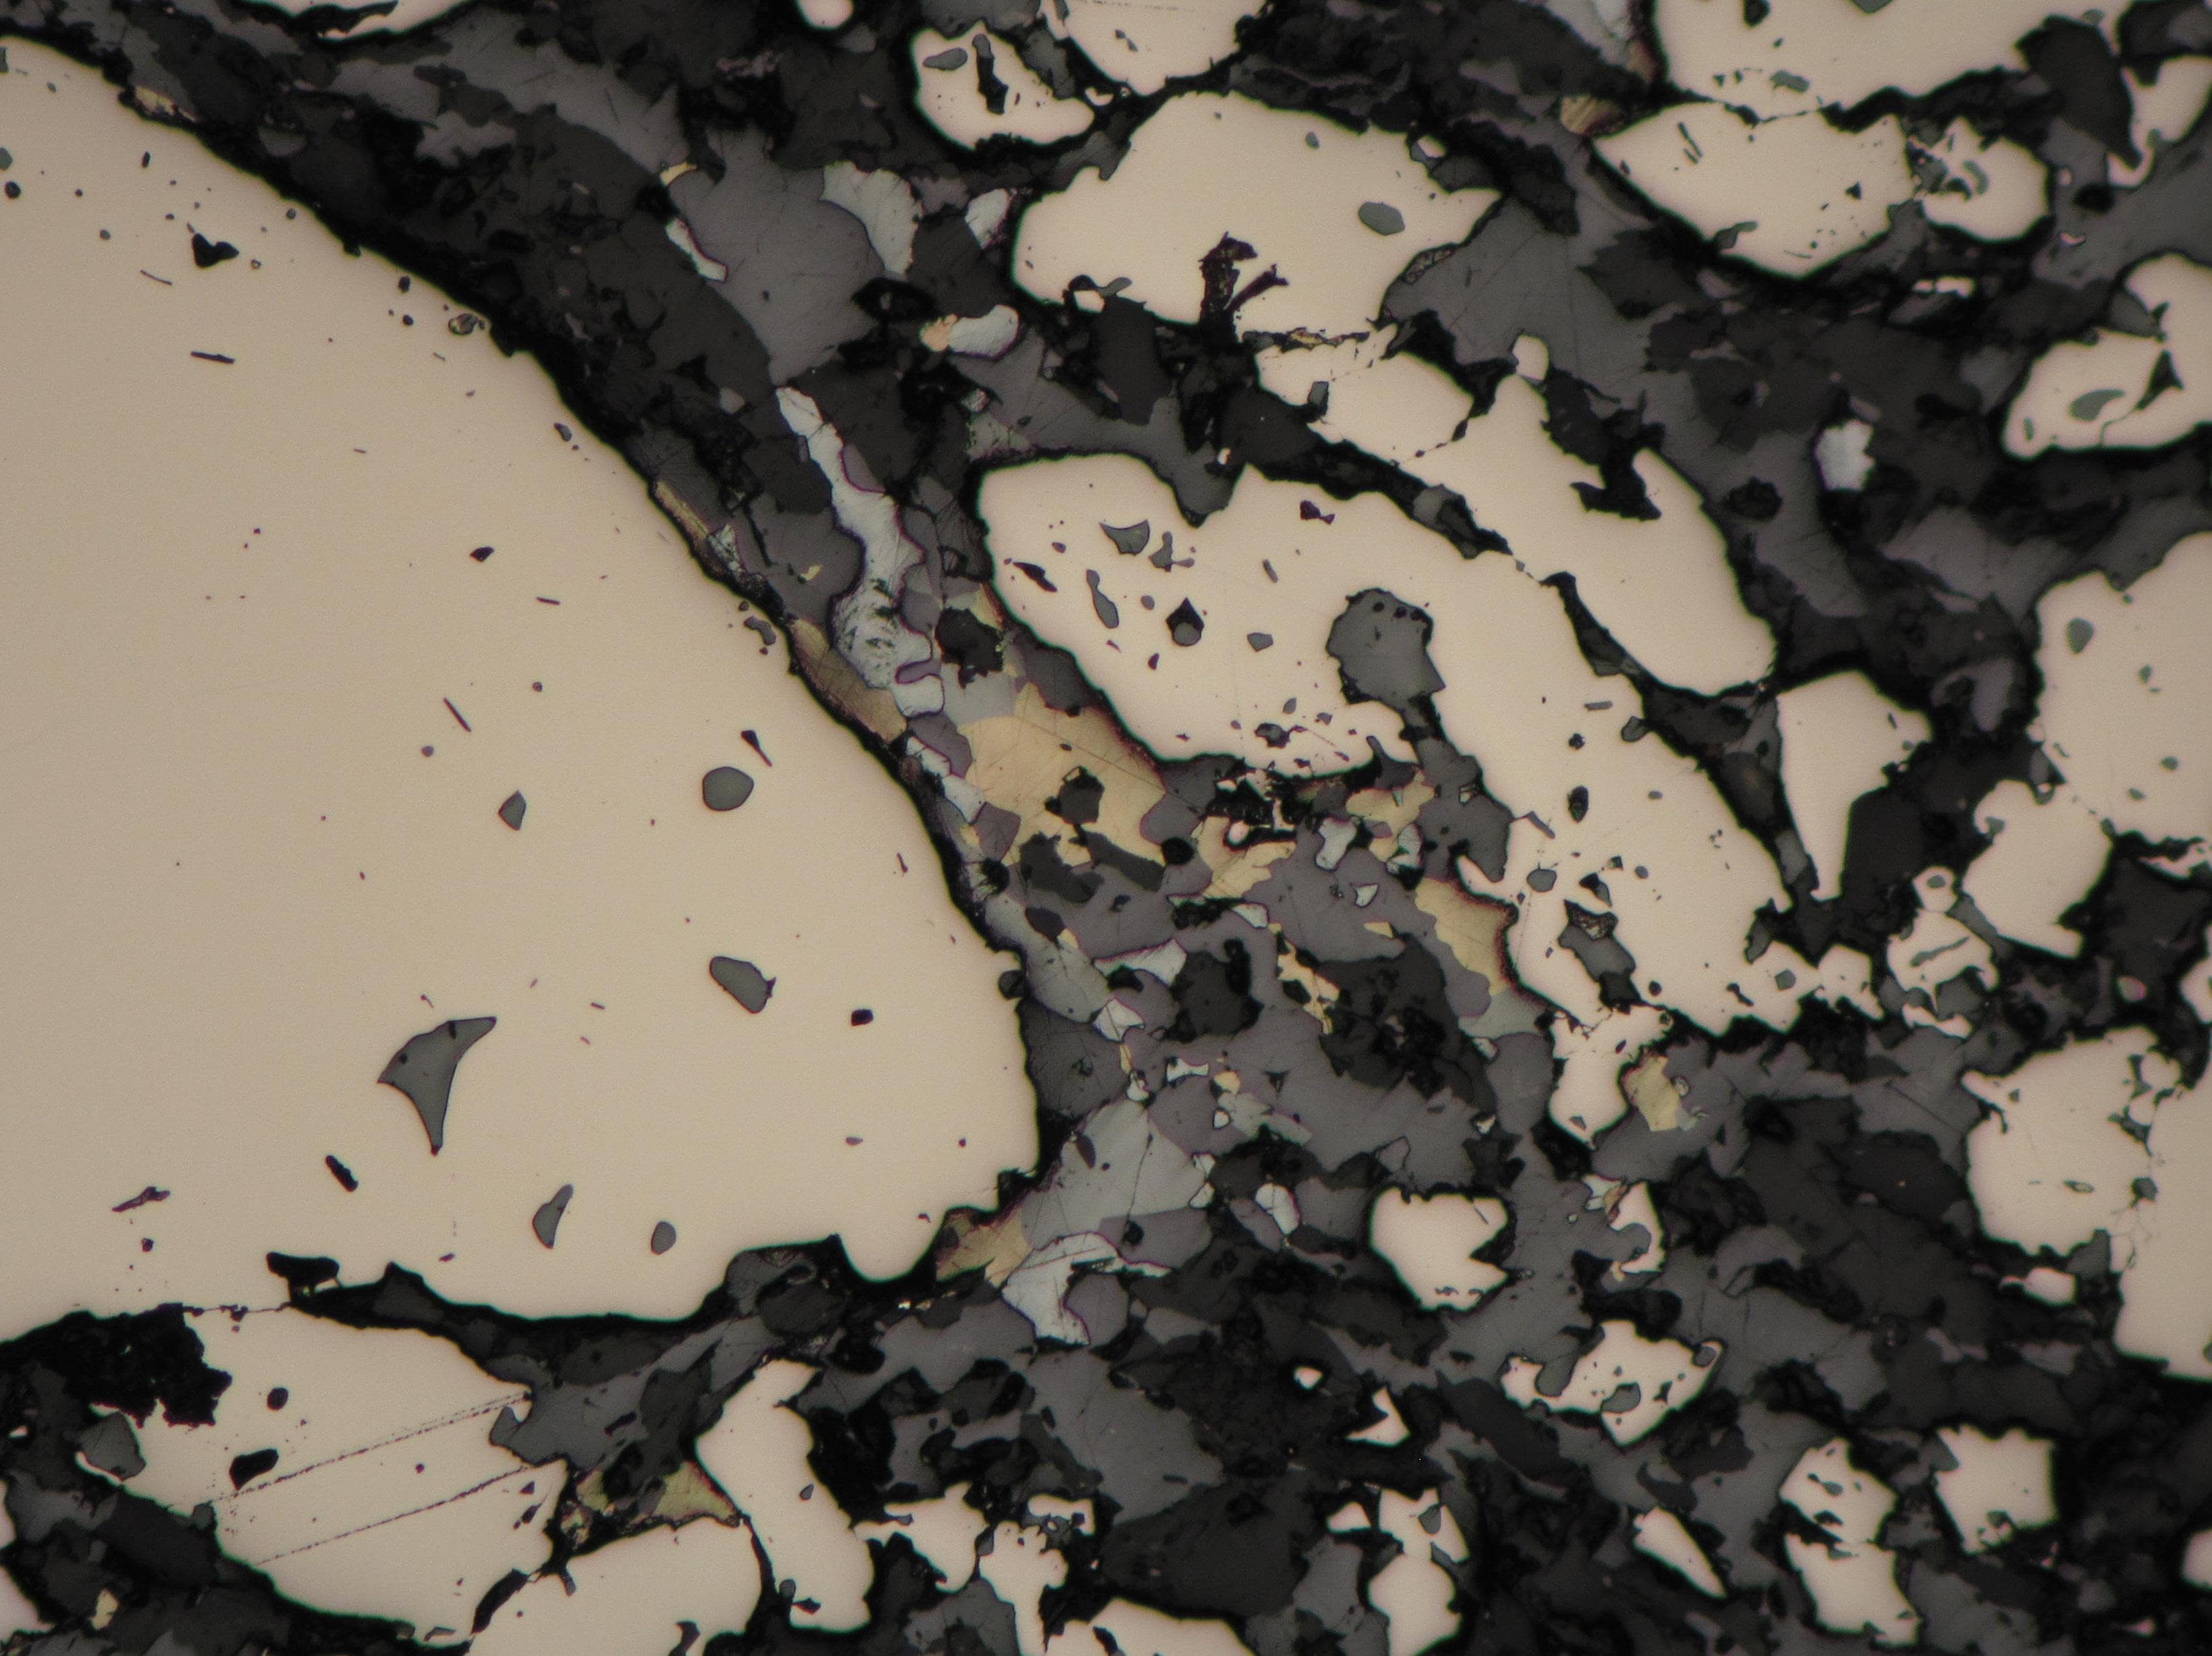
\includegraphics[width=.9\linewidth]{pics/image_7_src.jpg}
  \caption{Исходное изображение}
  \label{fig:sfig2_1}
\end{subfigure}%
\begin{subfigure}{.33\textwidth}
  \centering
  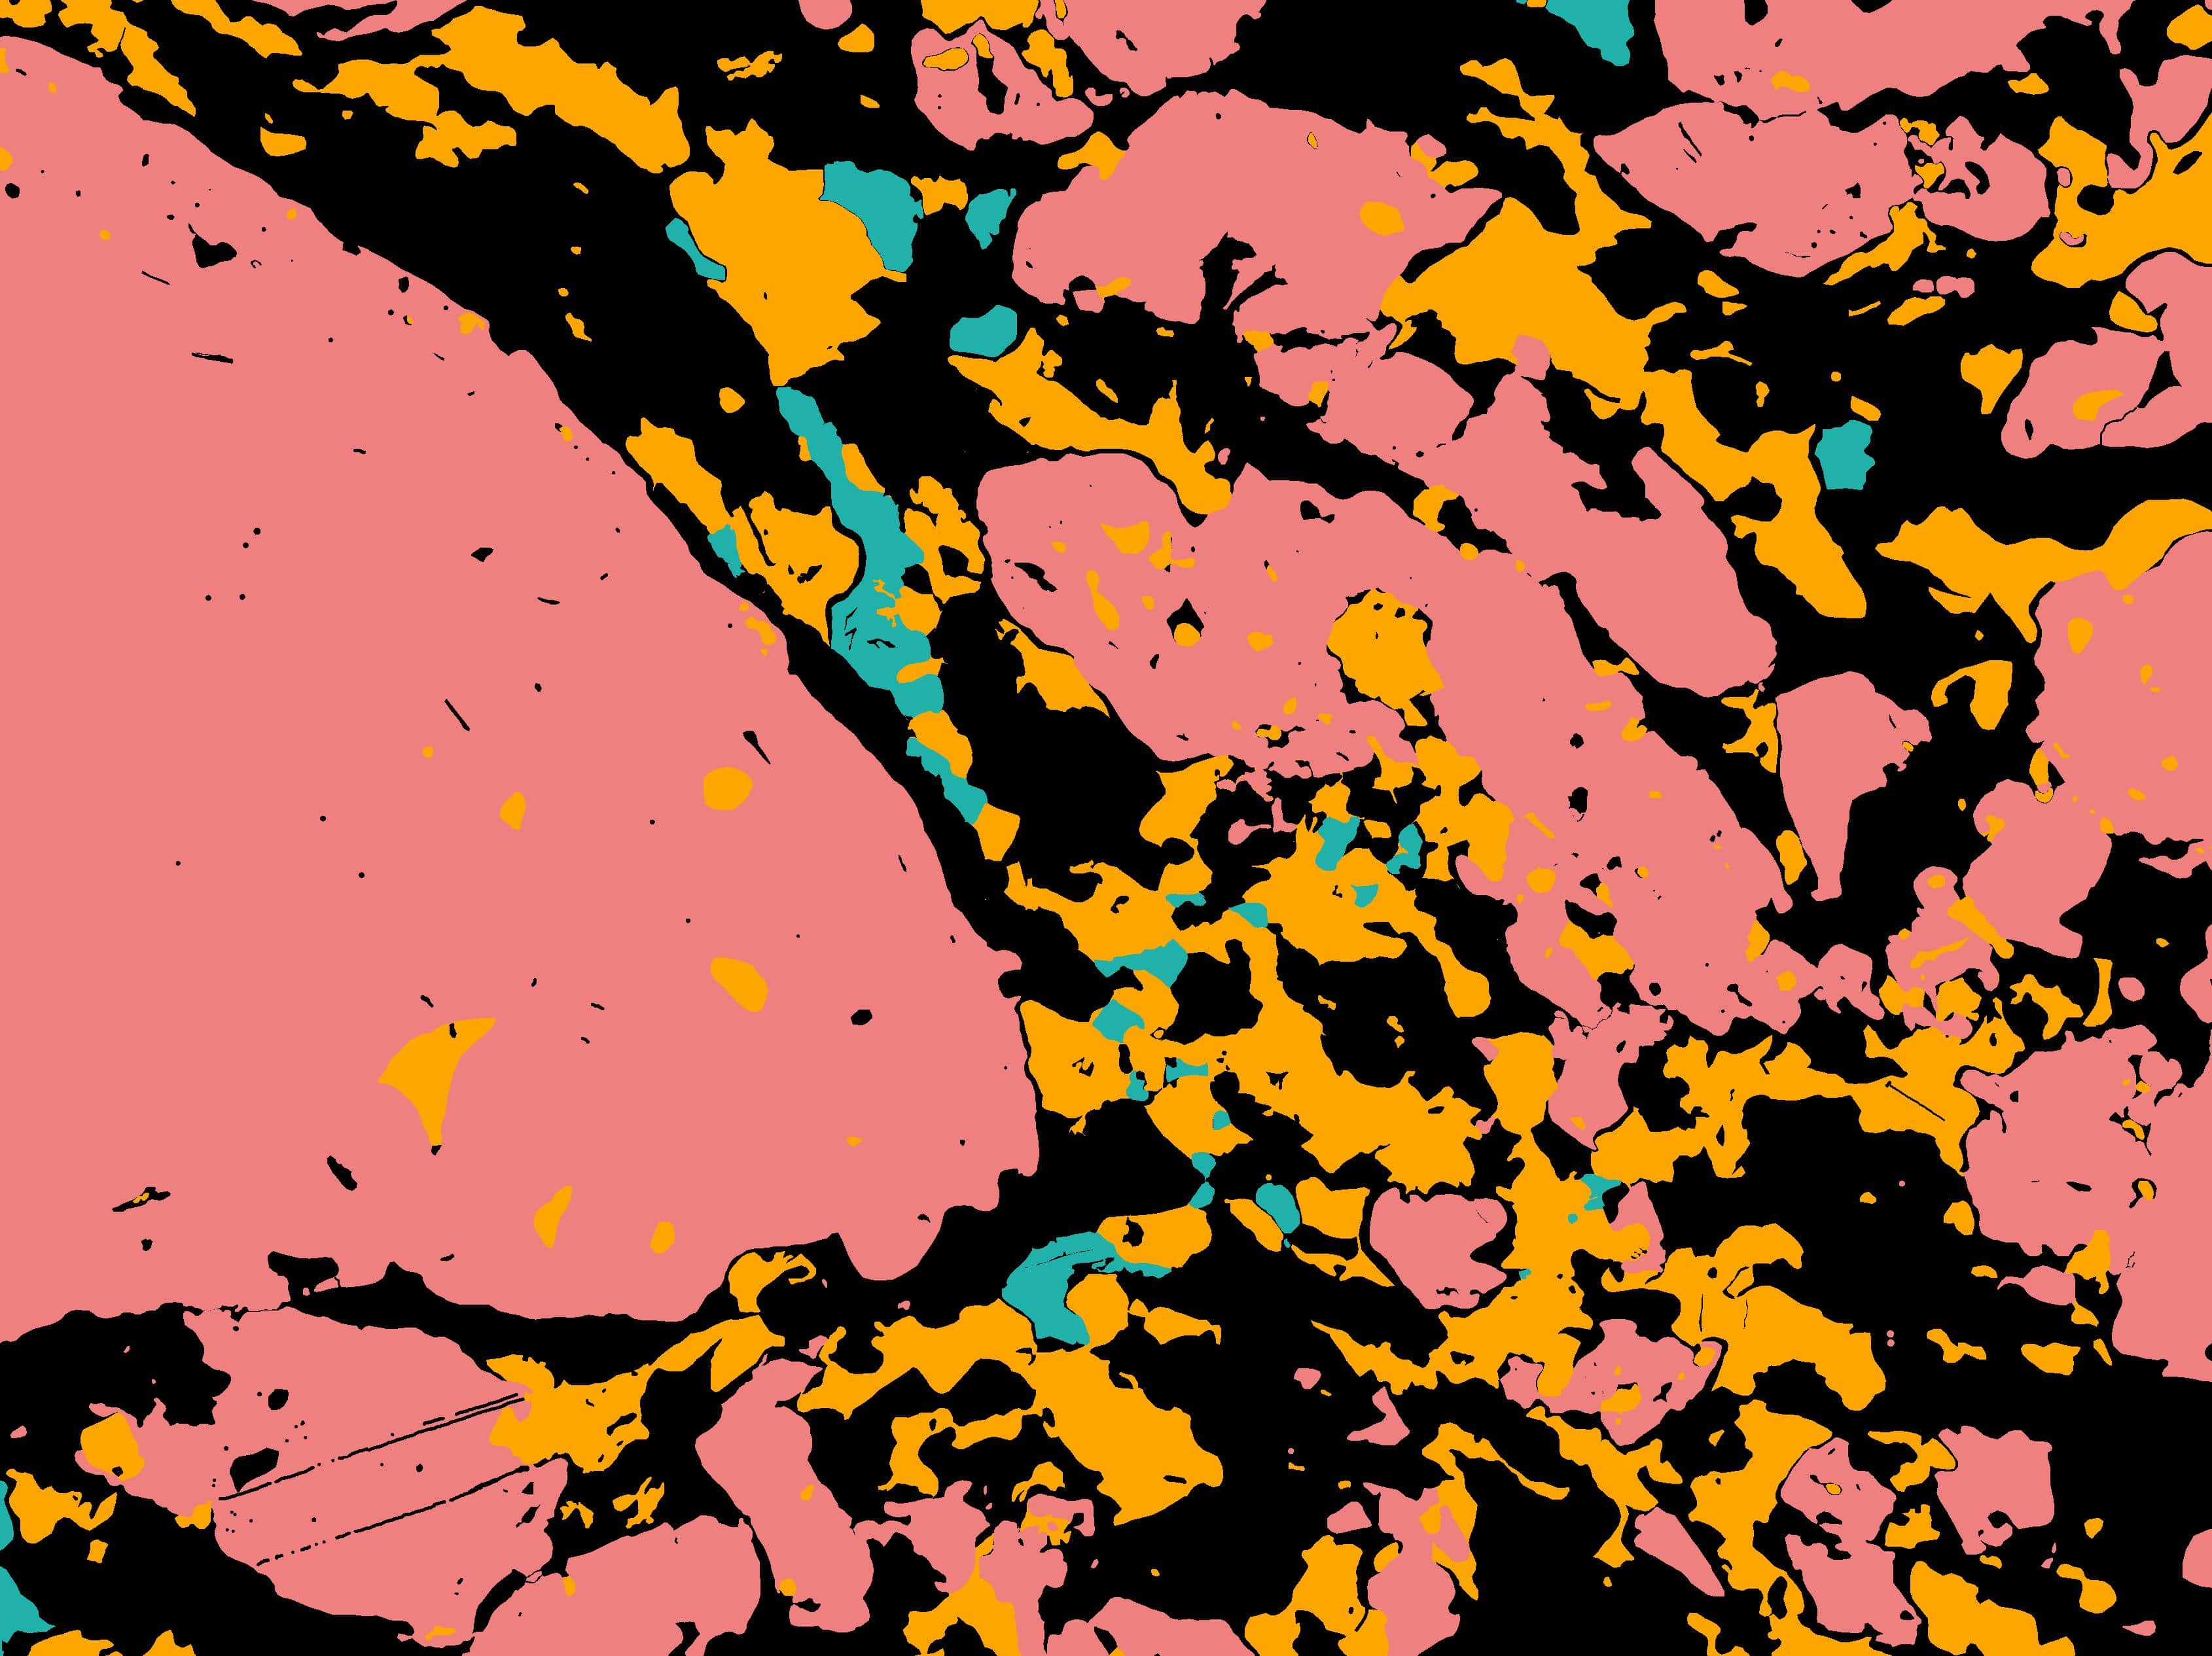
\includegraphics[width=.9\linewidth]{pics/image_7_gt.jpg}
  \caption{Экспертная разметка}
  \label{fig:sfig2_2}
\end{subfigure}%
\begin{subfigure}{.33\textwidth}
  \centering
  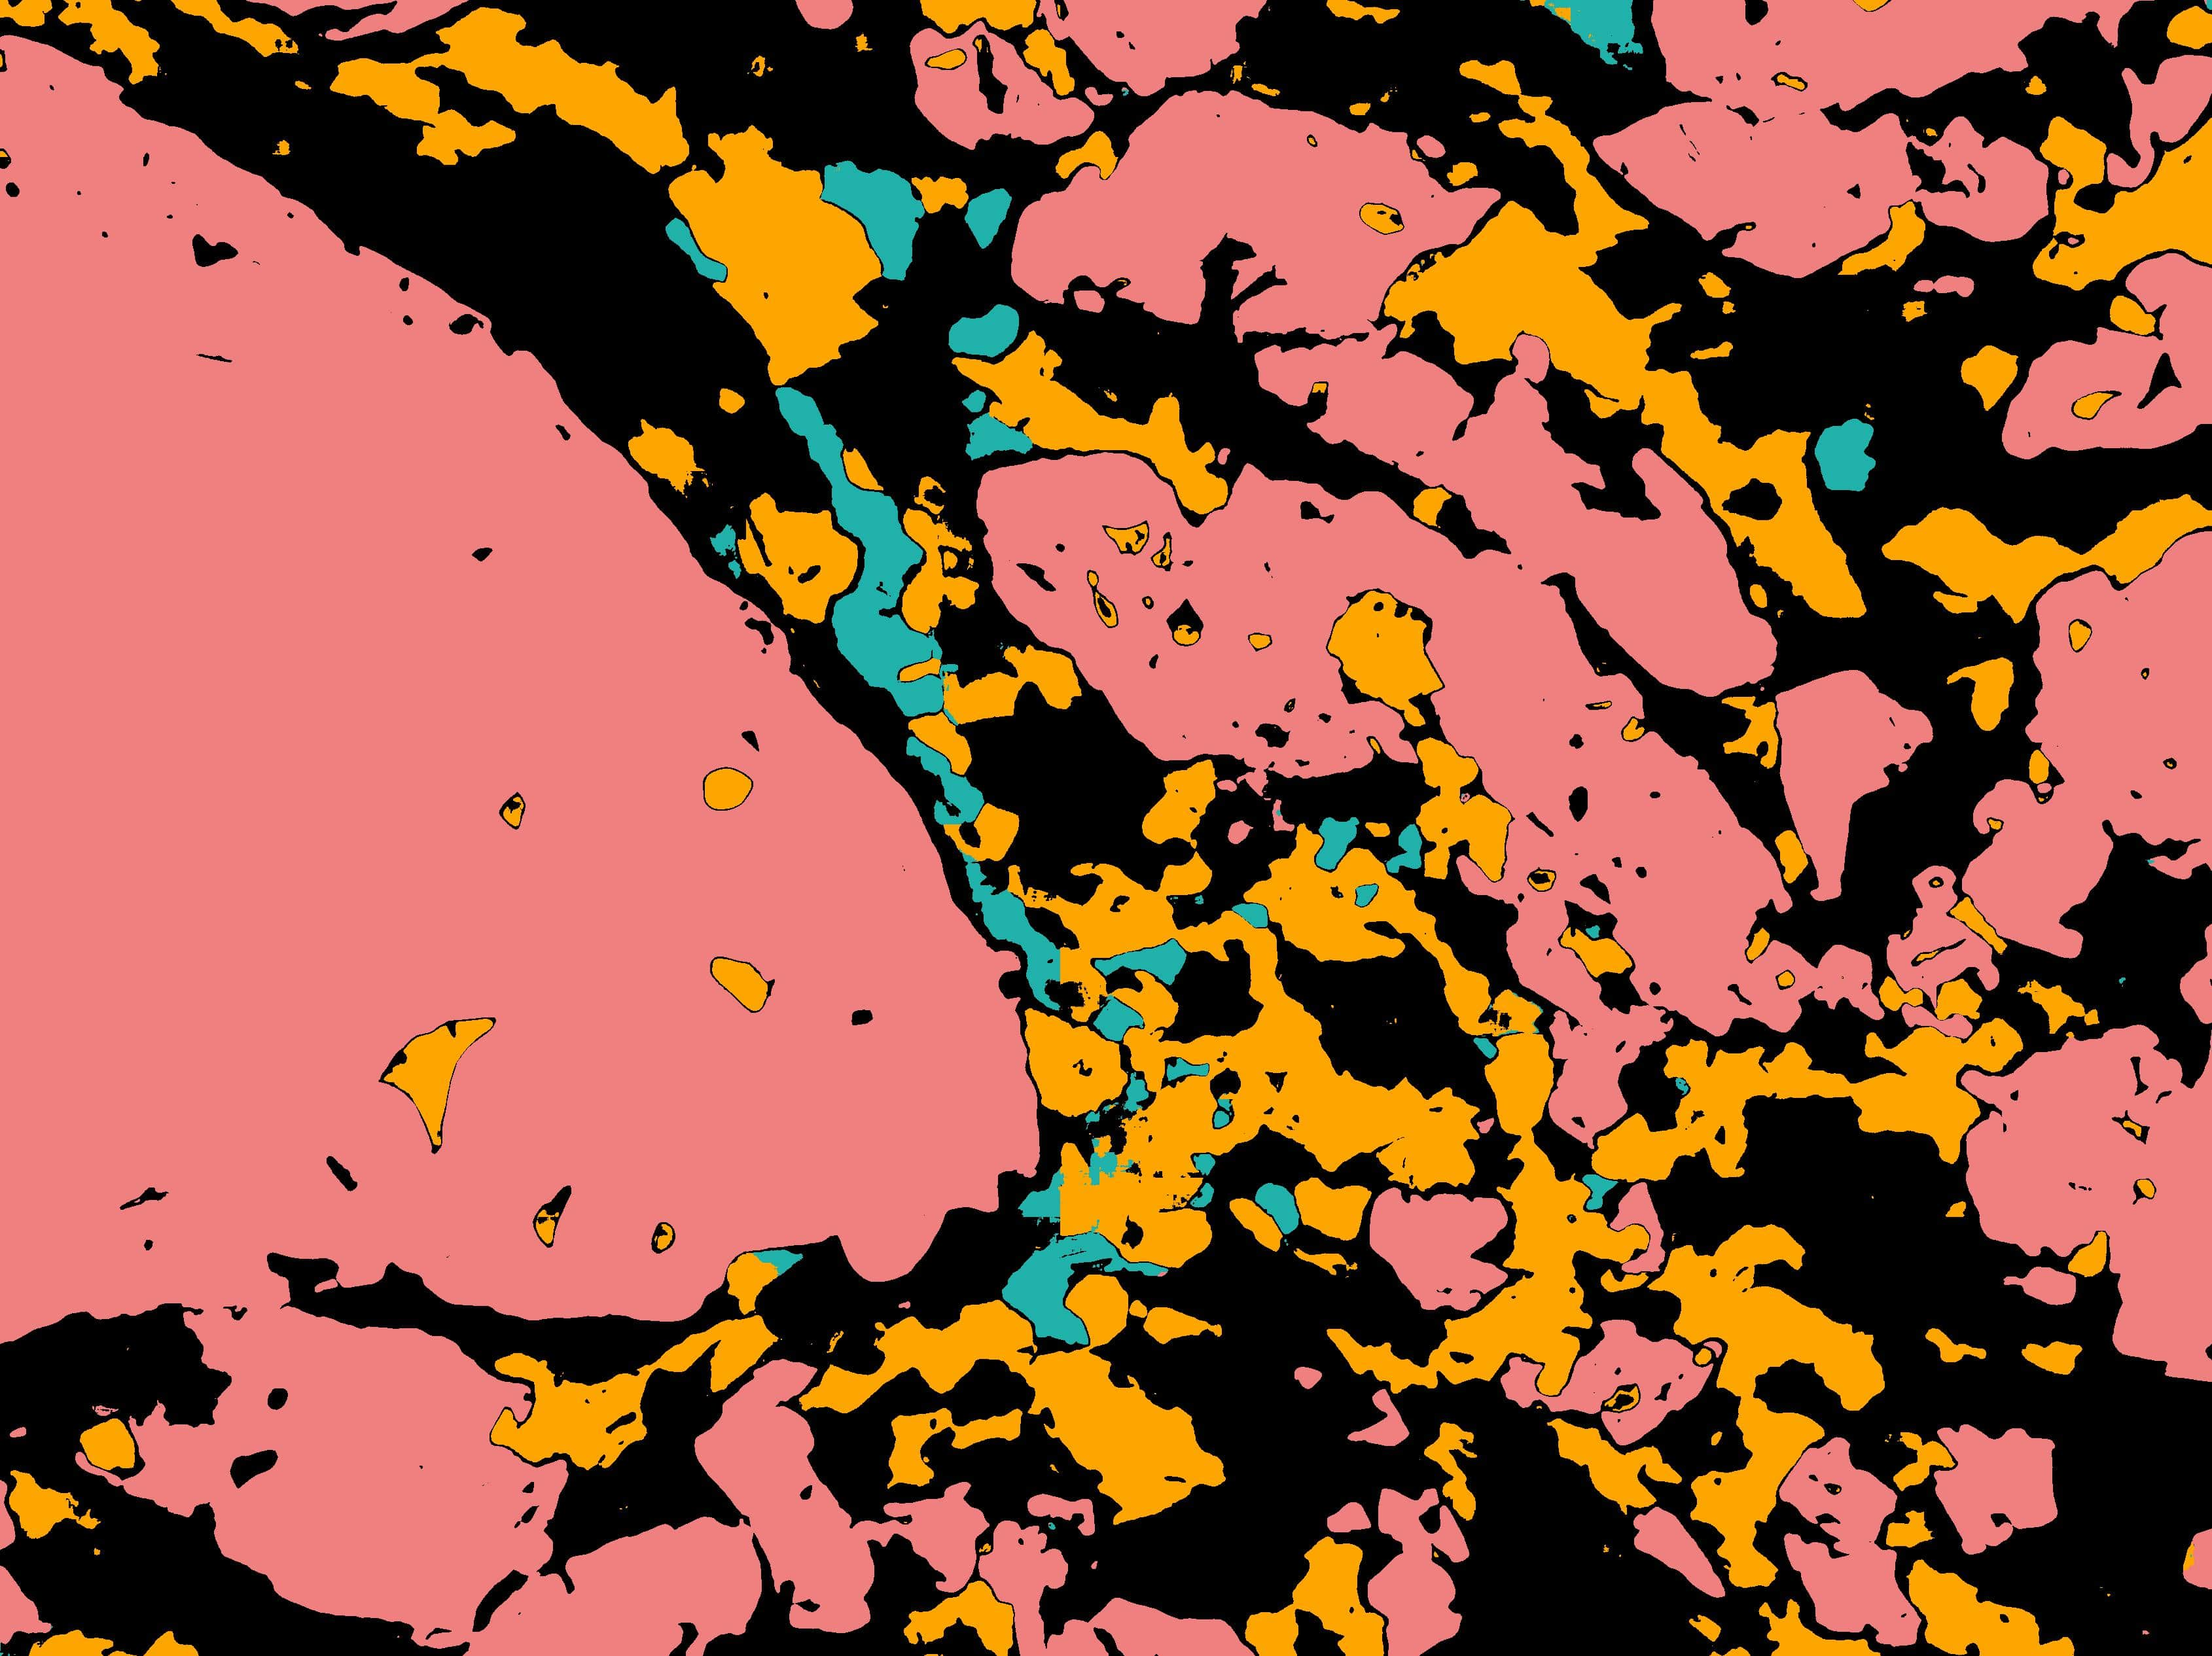
\includegraphics[width=.9\linewidth]{pics/image_7_pred.jpg}
  \caption{Предсказание}
  \label{fig:sfig2_3}
\end{subfigure} \\
\centering
\begin{subfigure}{.33\textwidth}
  \centering
  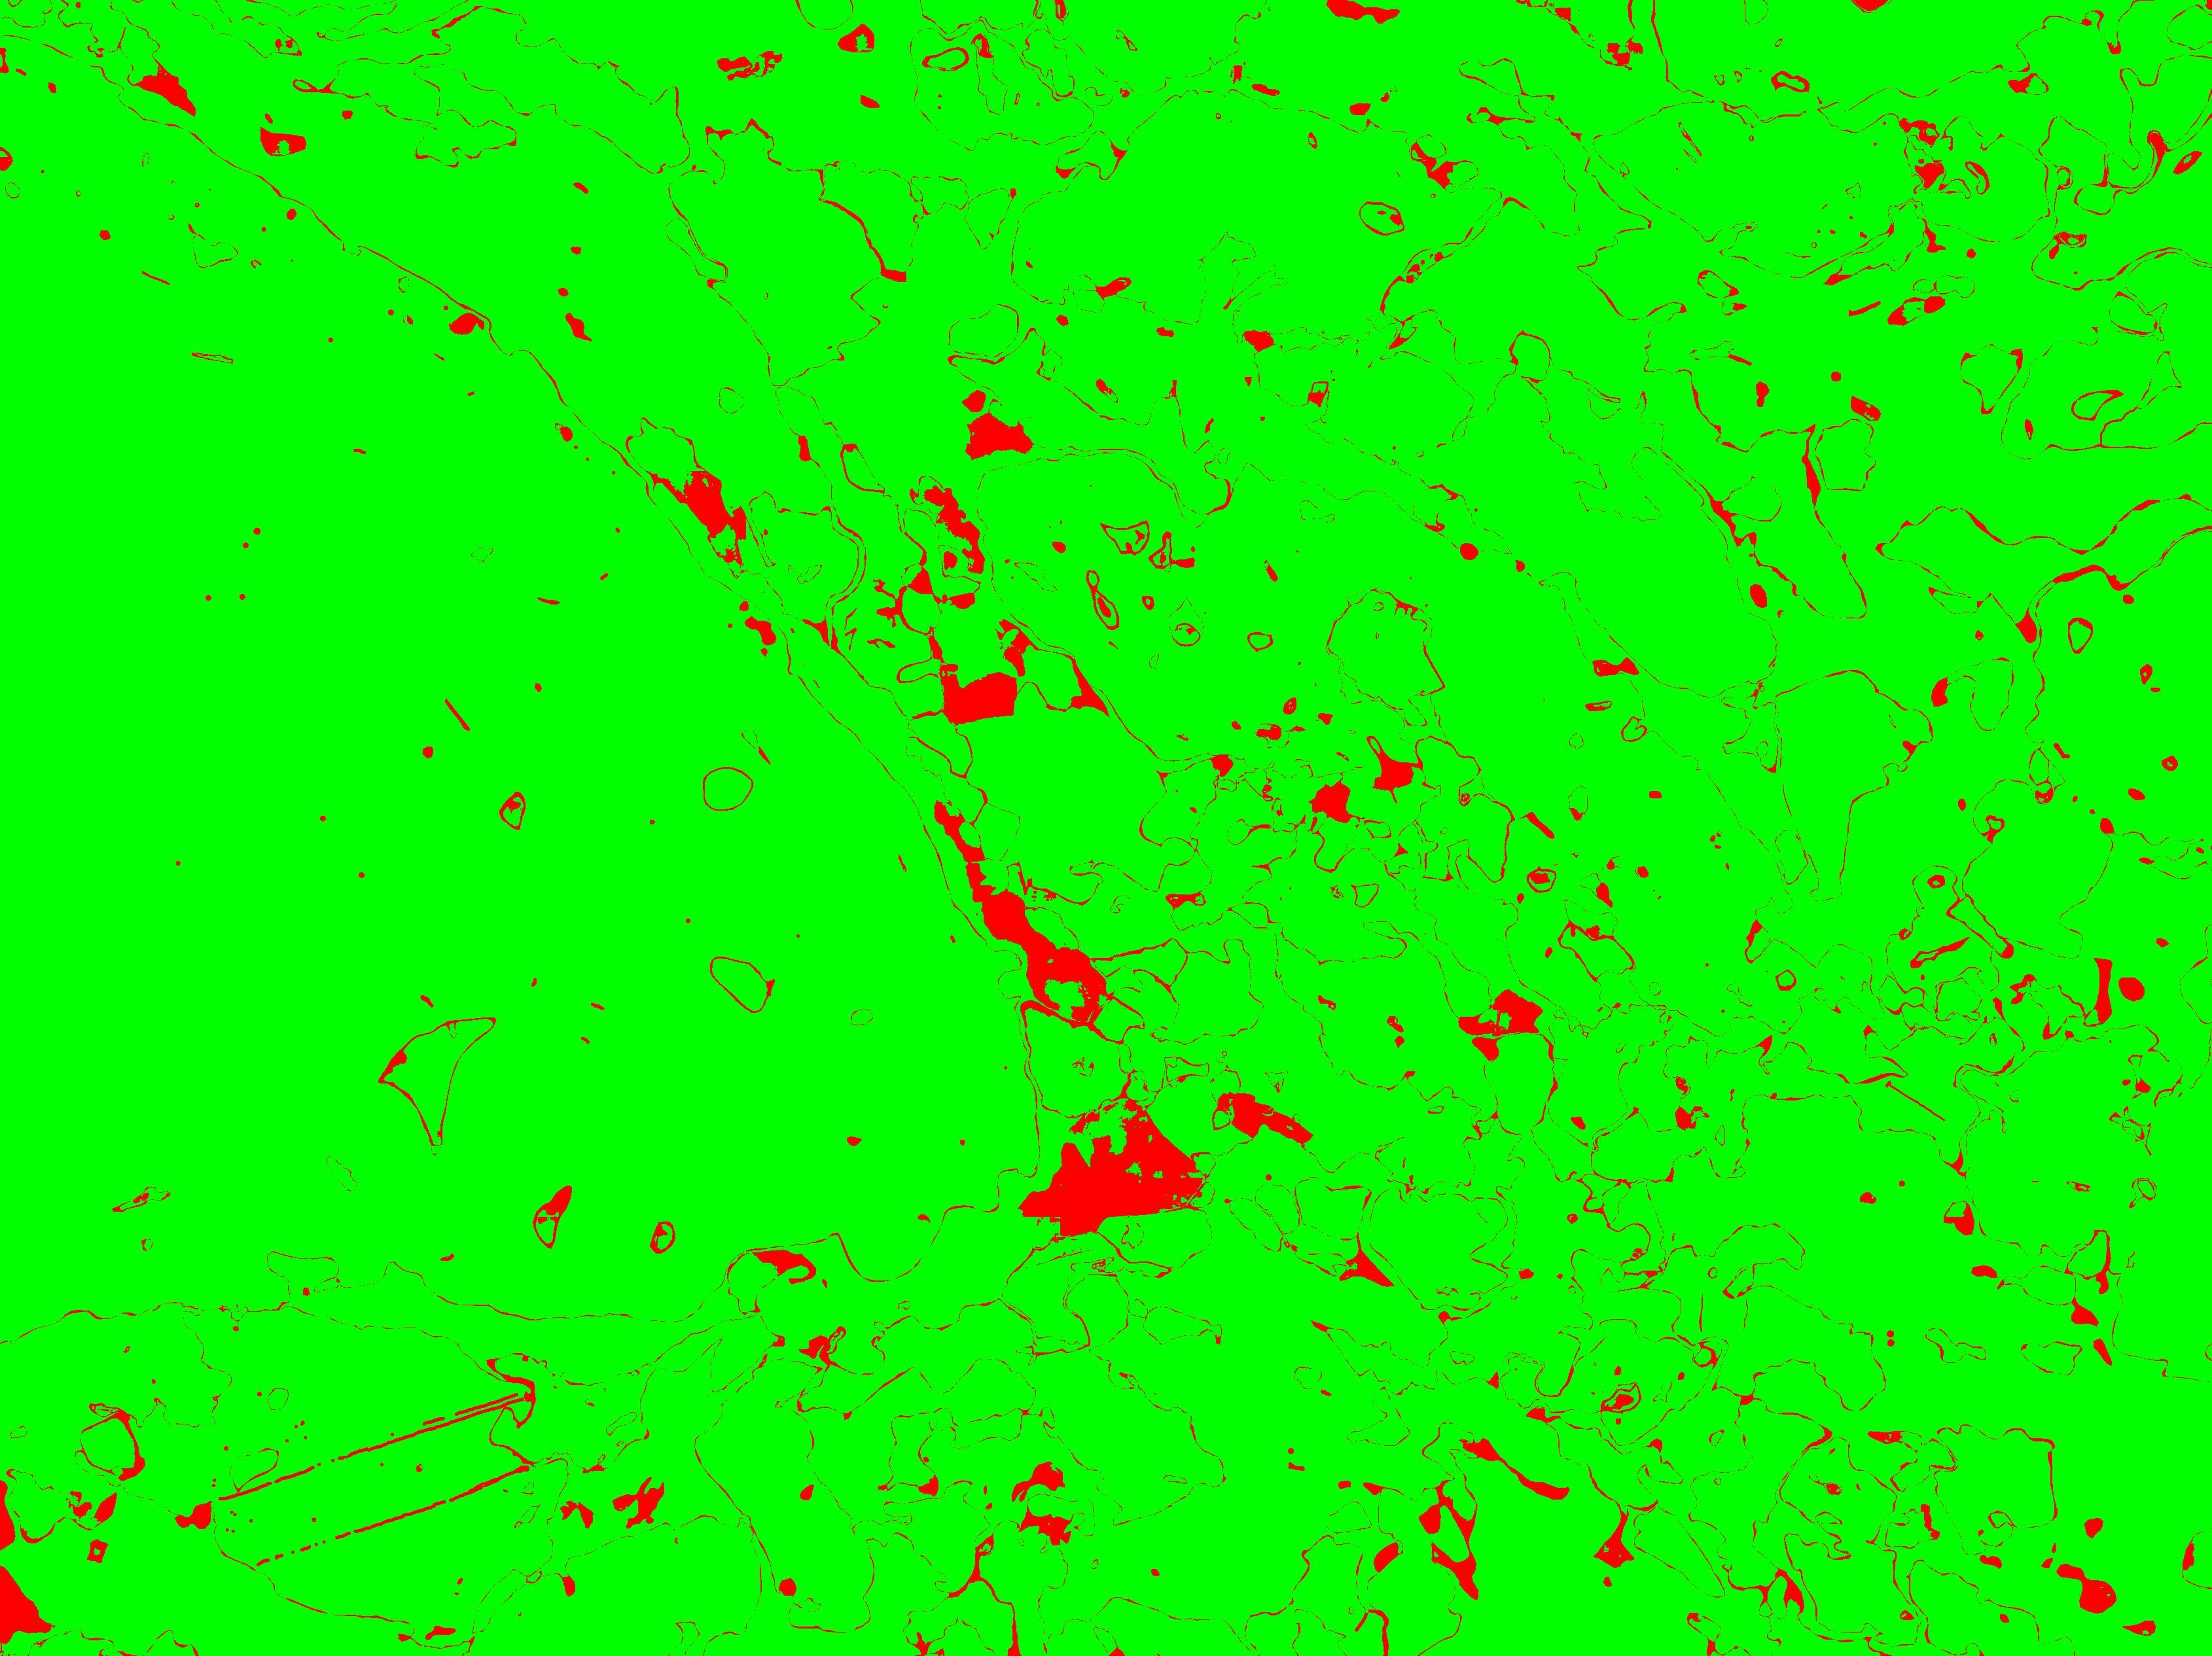
\includegraphics[width=.9\linewidth]{pics/image_7_error.jpg}
  \caption{Карта ошибок}
  \label{fig:sfig2_4}
\end{subfigure}%
\begin{subfigure}{.33\textwidth}
  \centering
  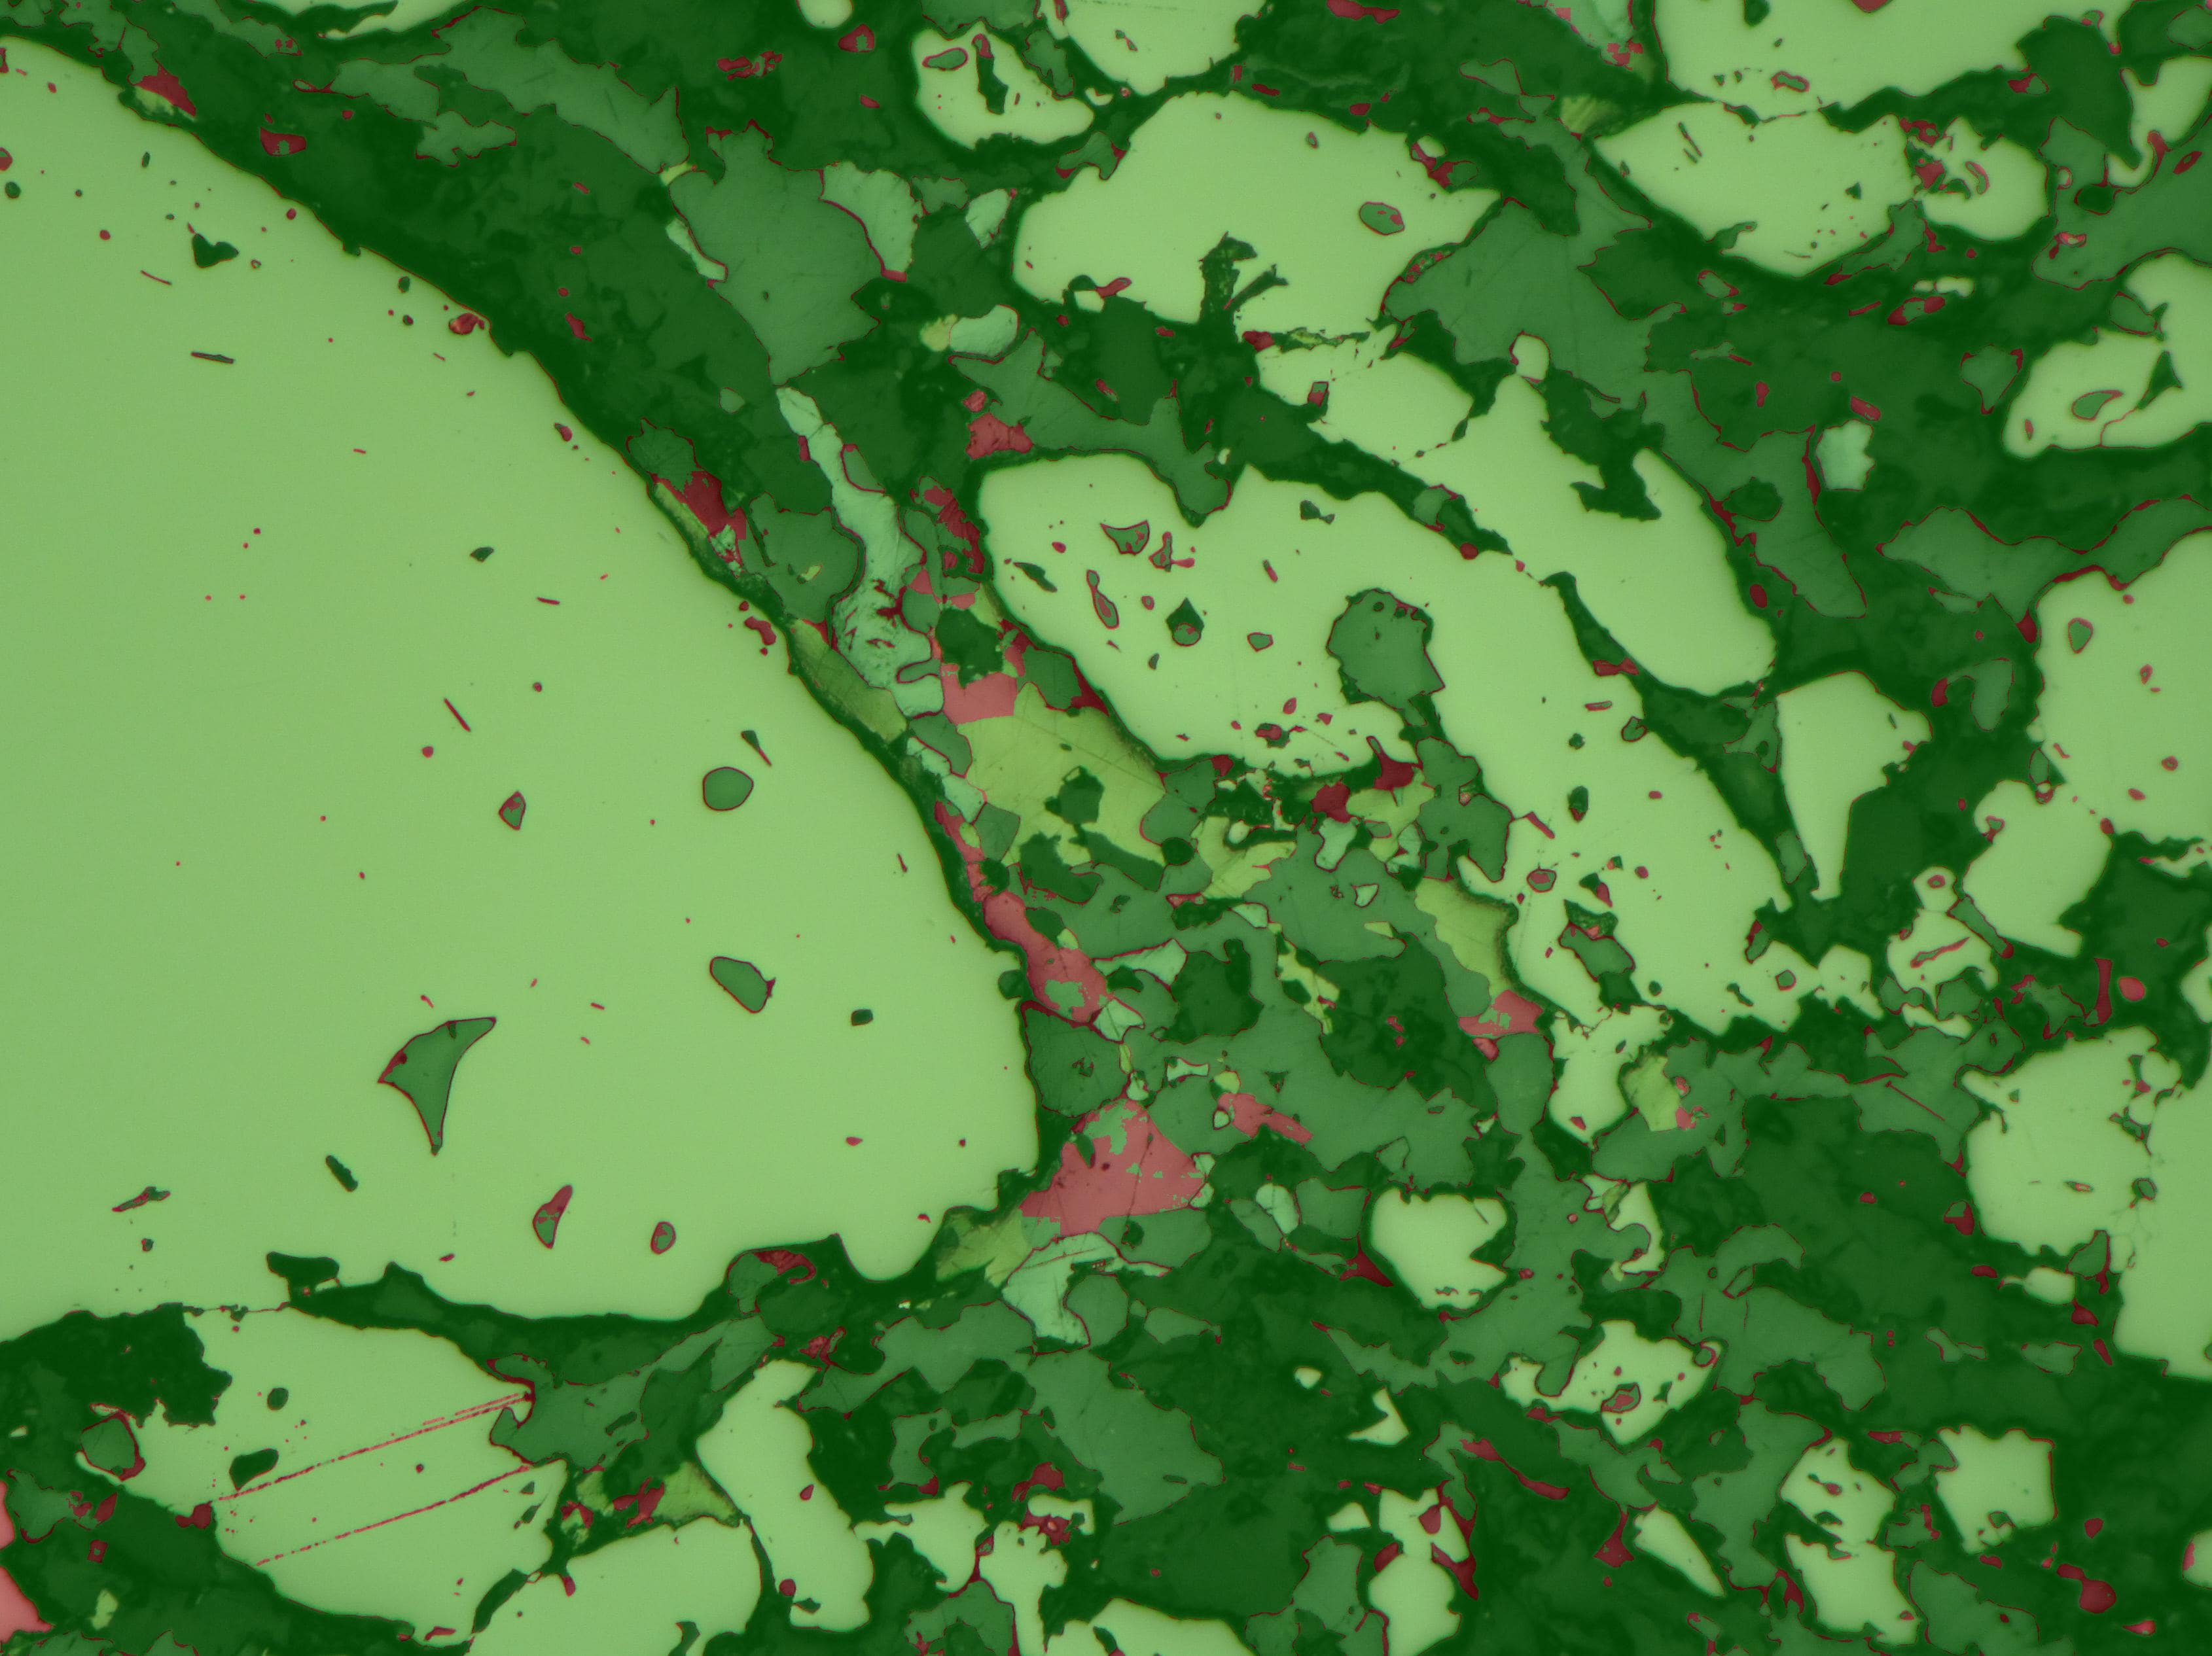
\includegraphics[width=.9\linewidth]{pics/image_7_overlay.jpg}
  \caption{Карта ошибок + исходное}
  \label{fig:sfig2_5}
\end{subfigure}
\caption{Тестовое изображение №2}
\label{fig:pred2}
\end{figure}

Тестовое изображение №2 было распознано правильно на 95.325\%, каждый из классов был распознан: \\
\begin{enumerate}[nosep]
    \item Background: 94.511\%
    \item Sh: 85.962\%
    \item Py/Mrc: 99.335\%
    \item Gl: 88.949\%
\end{enumerate}{}
Мера качества IoU показала следующие результаты:
\begin{enumerate}[nosep]
    \item Background: 0.86
    \item Sh: 0.78
    \item Py/Mrc: 0.97
    \item Gl: 0.67
\end{enumerate}{}

\begin{figure}[H]
\begin{subfigure}{.33\textwidth}
  \centering
  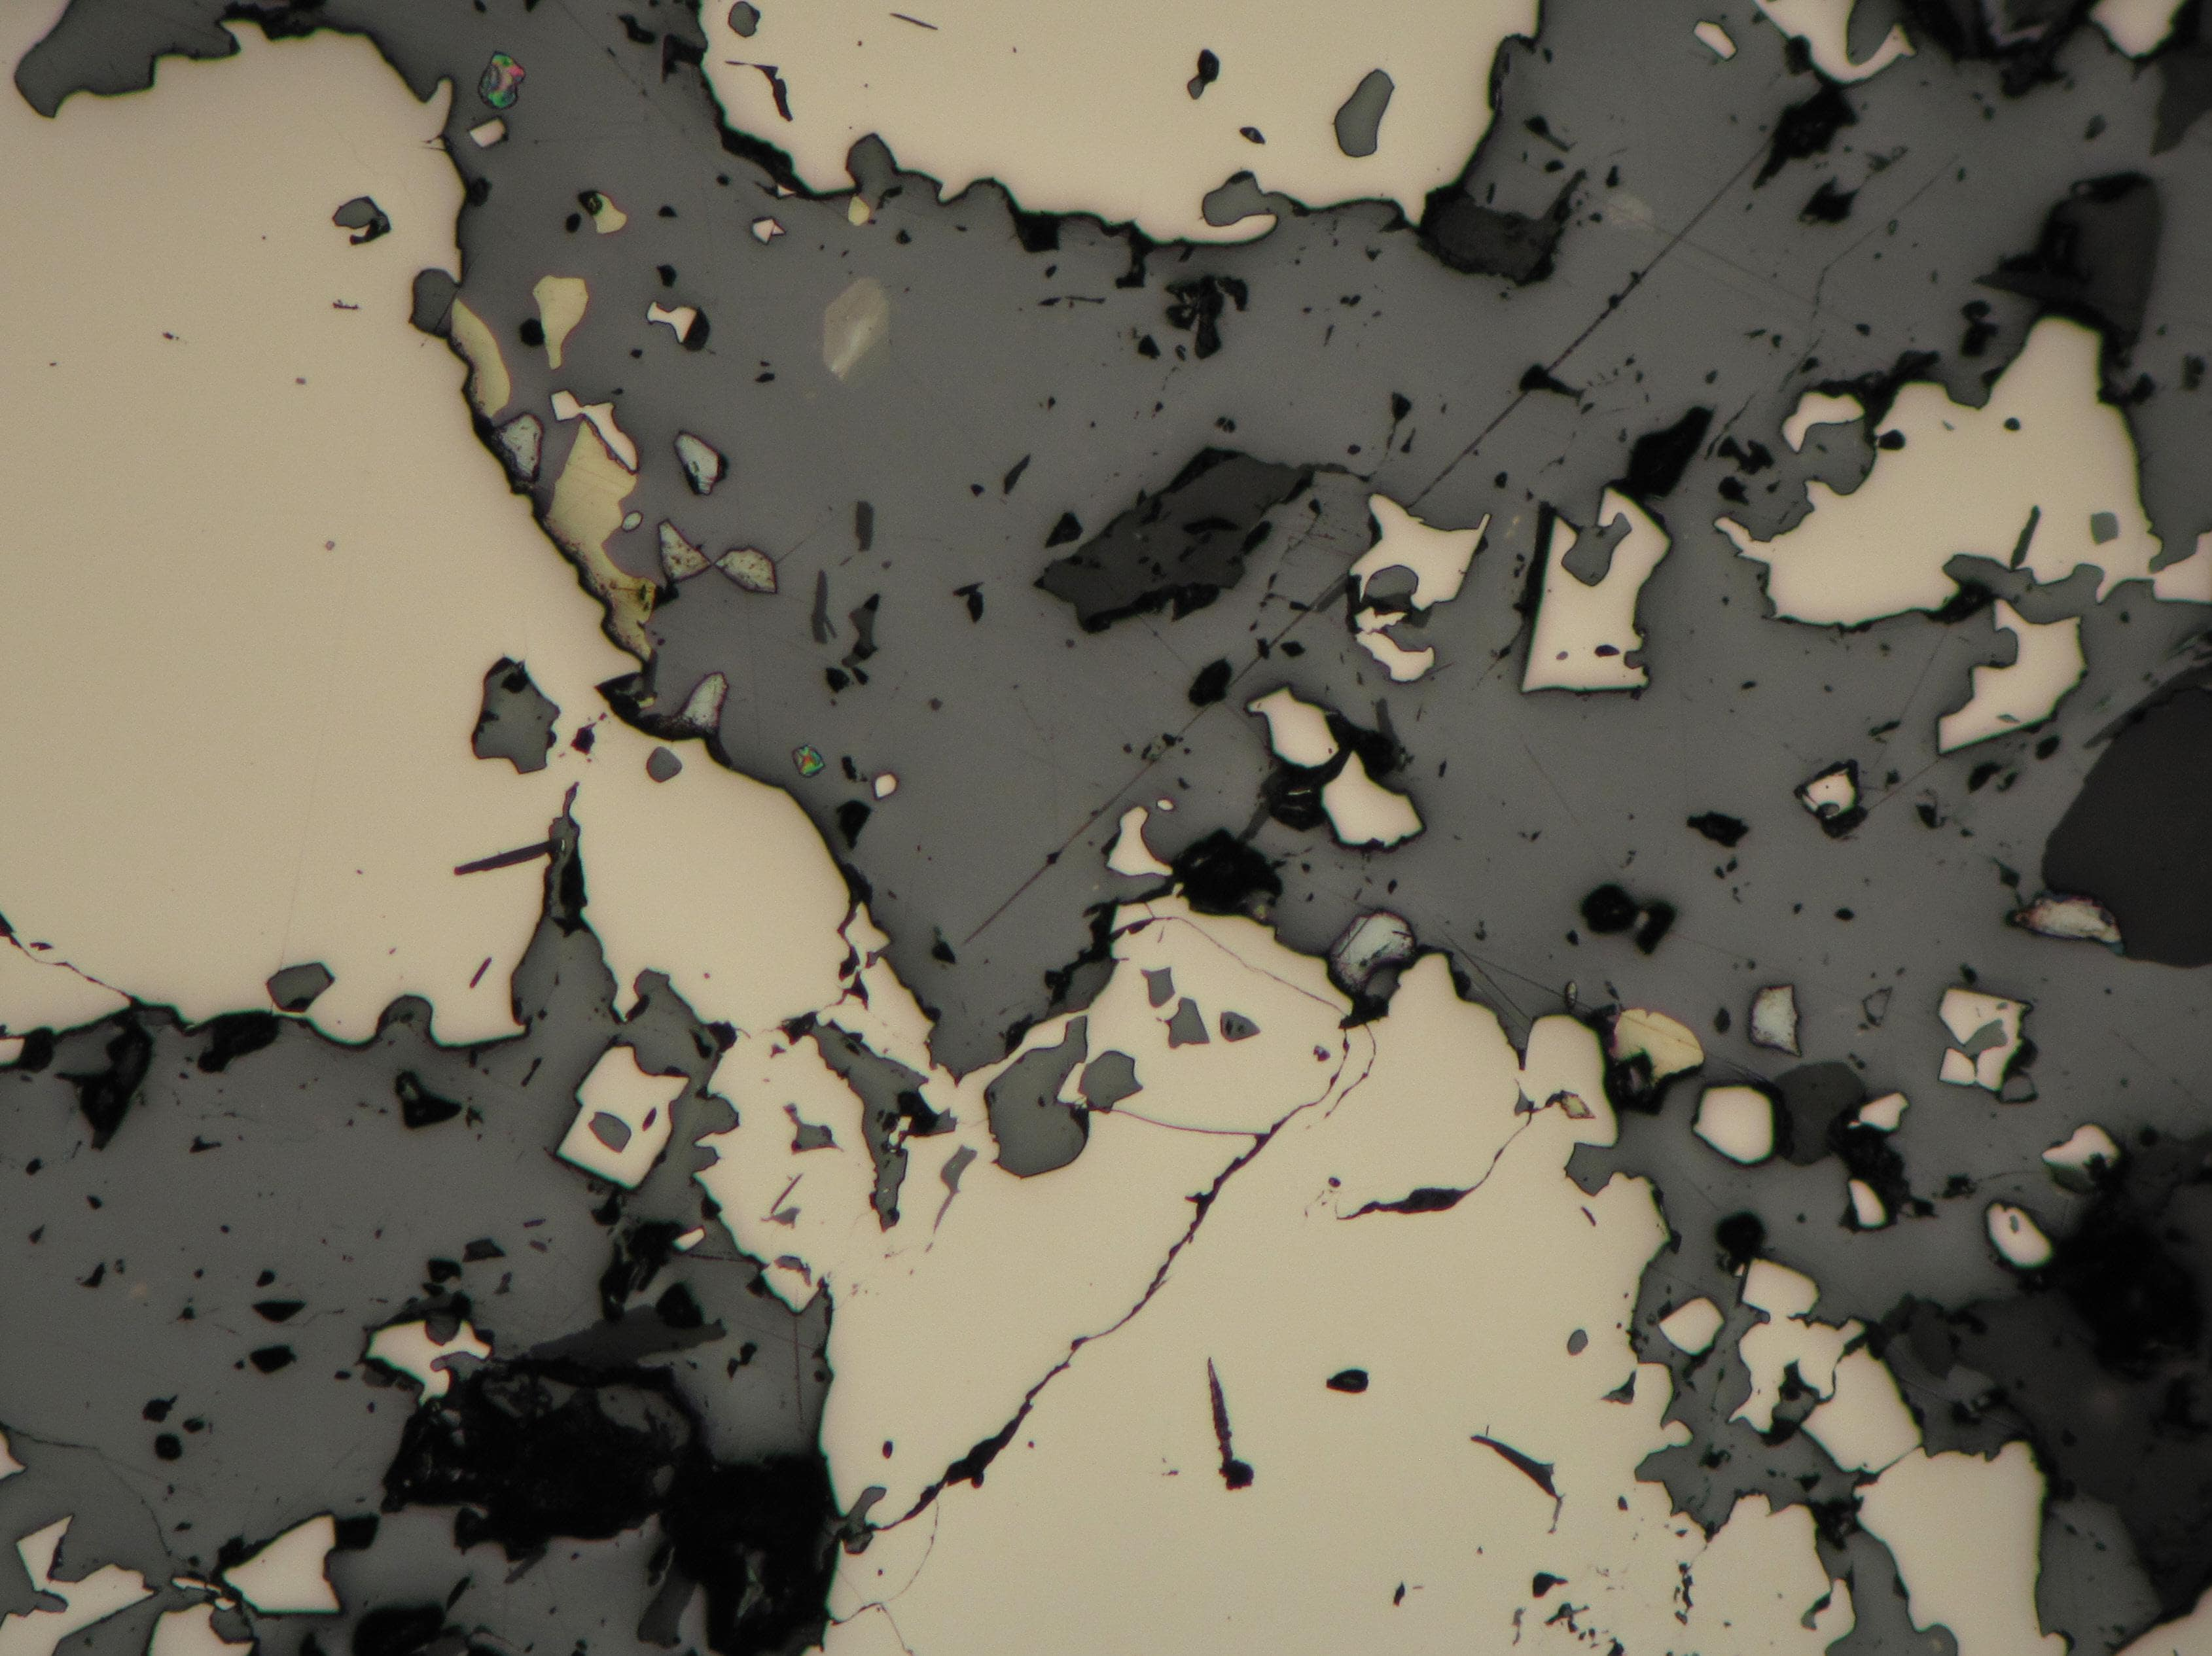
\includegraphics[width=.9\linewidth]{pics/image_5_src.jpg}
  \caption{Исходное изображение}
  \label{fig:sfig3_1}
\end{subfigure}%
\begin{subfigure}{.33\textwidth}
  \centering
  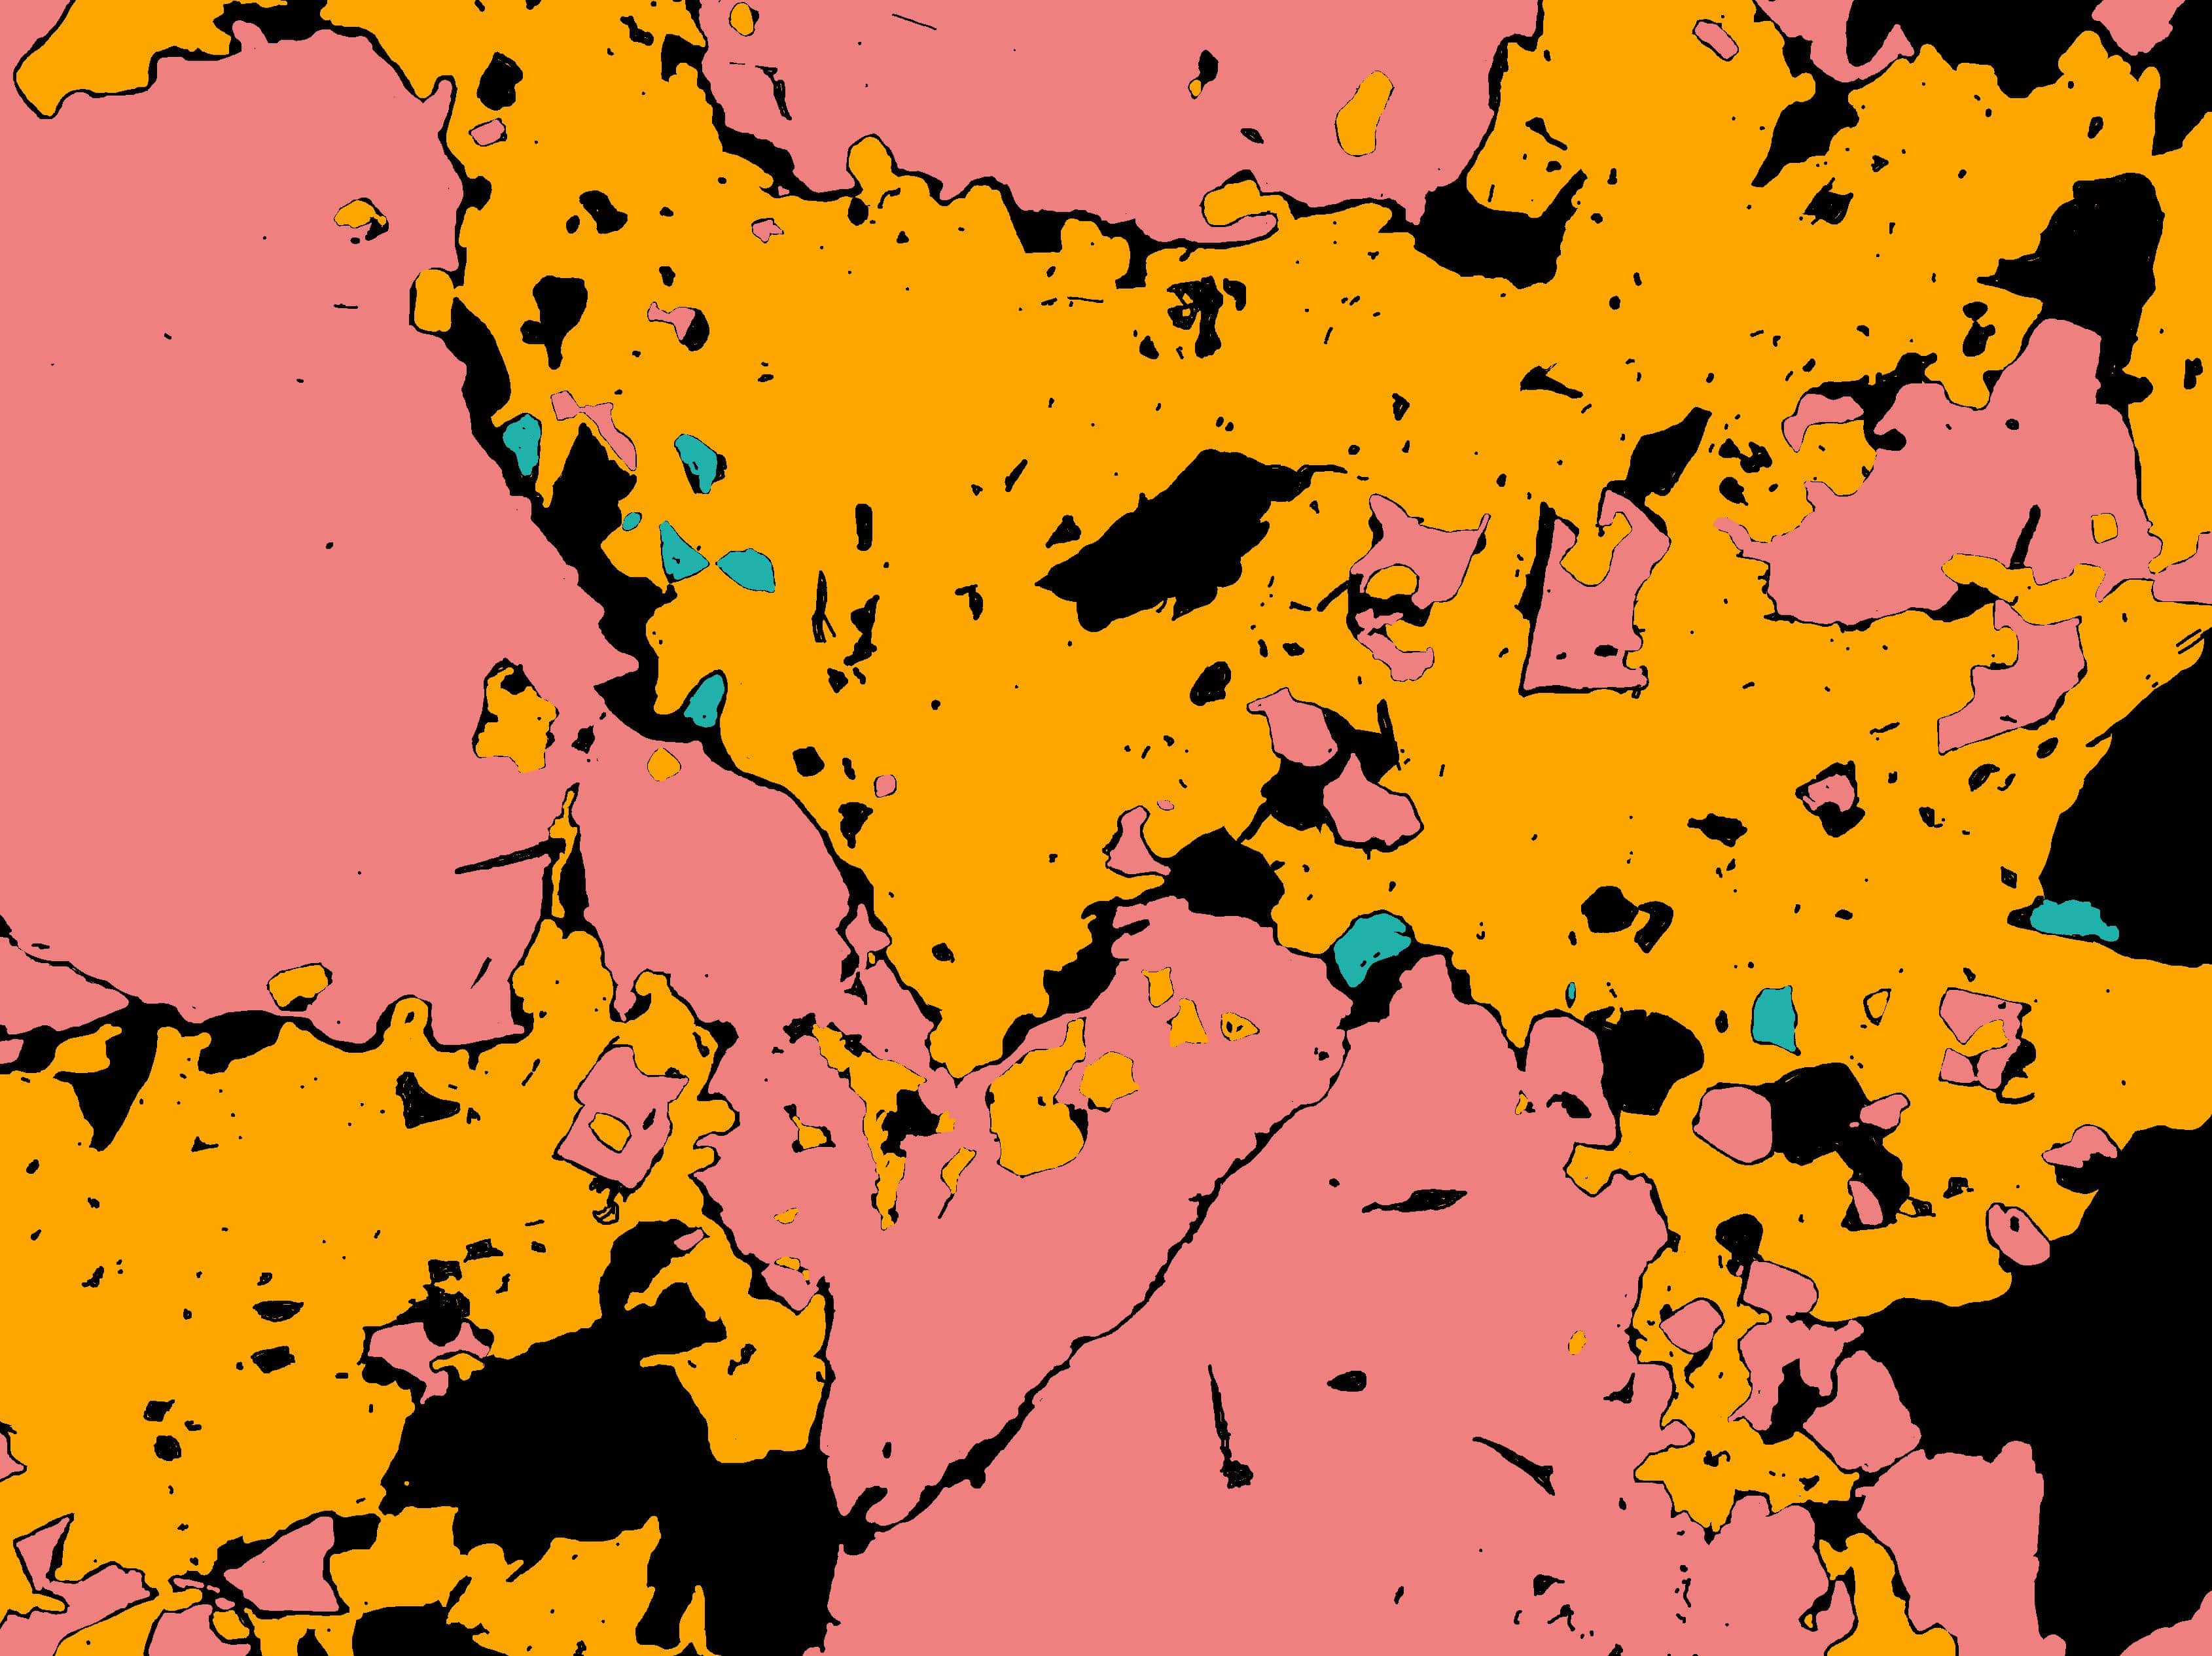
\includegraphics[width=.9\linewidth]{pics/image_5_gt.jpg}
  \caption{Экспертная разметка}
  \label{fig:sfig3_2}
\end{subfigure}%
\begin{subfigure}{.33\textwidth}
  \centering
  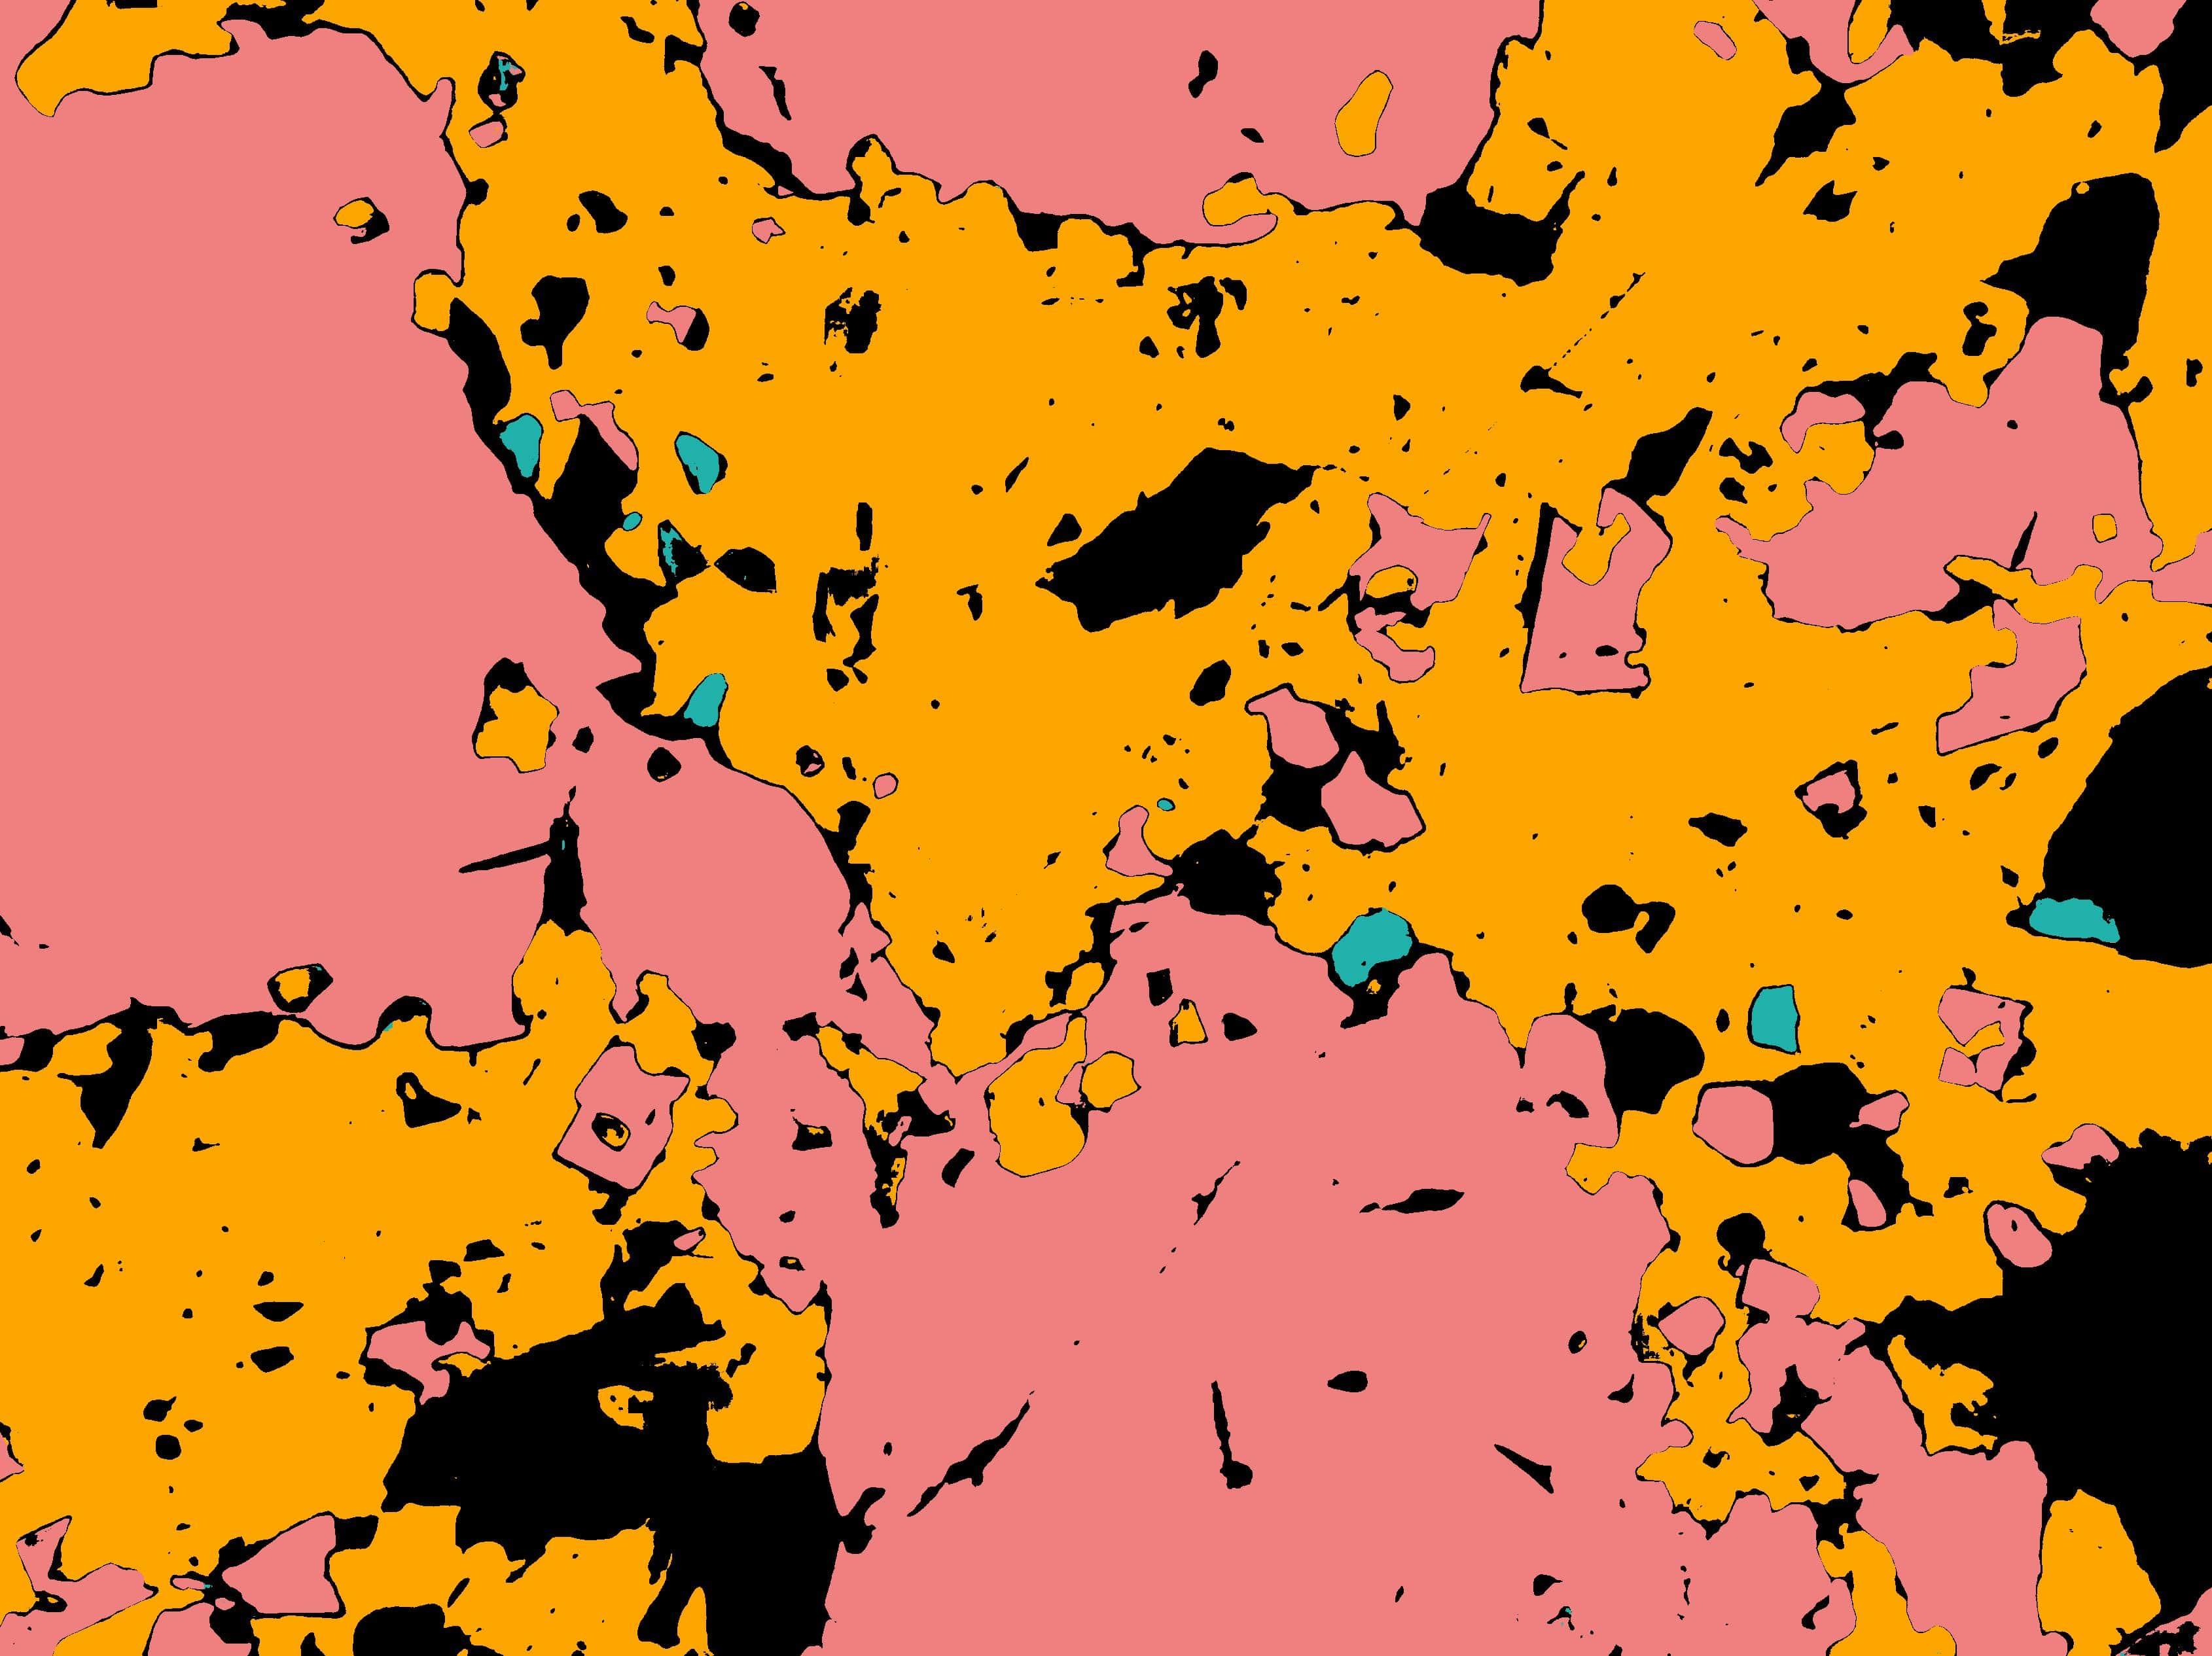
\includegraphics[width=.9\linewidth]{pics/image_5_pred.jpg}
  \caption{Предсказание}
  \label{fig:sfig3_3}
\end{subfigure} \\
\centering
\begin{subfigure}{.33\textwidth}
  \centering
  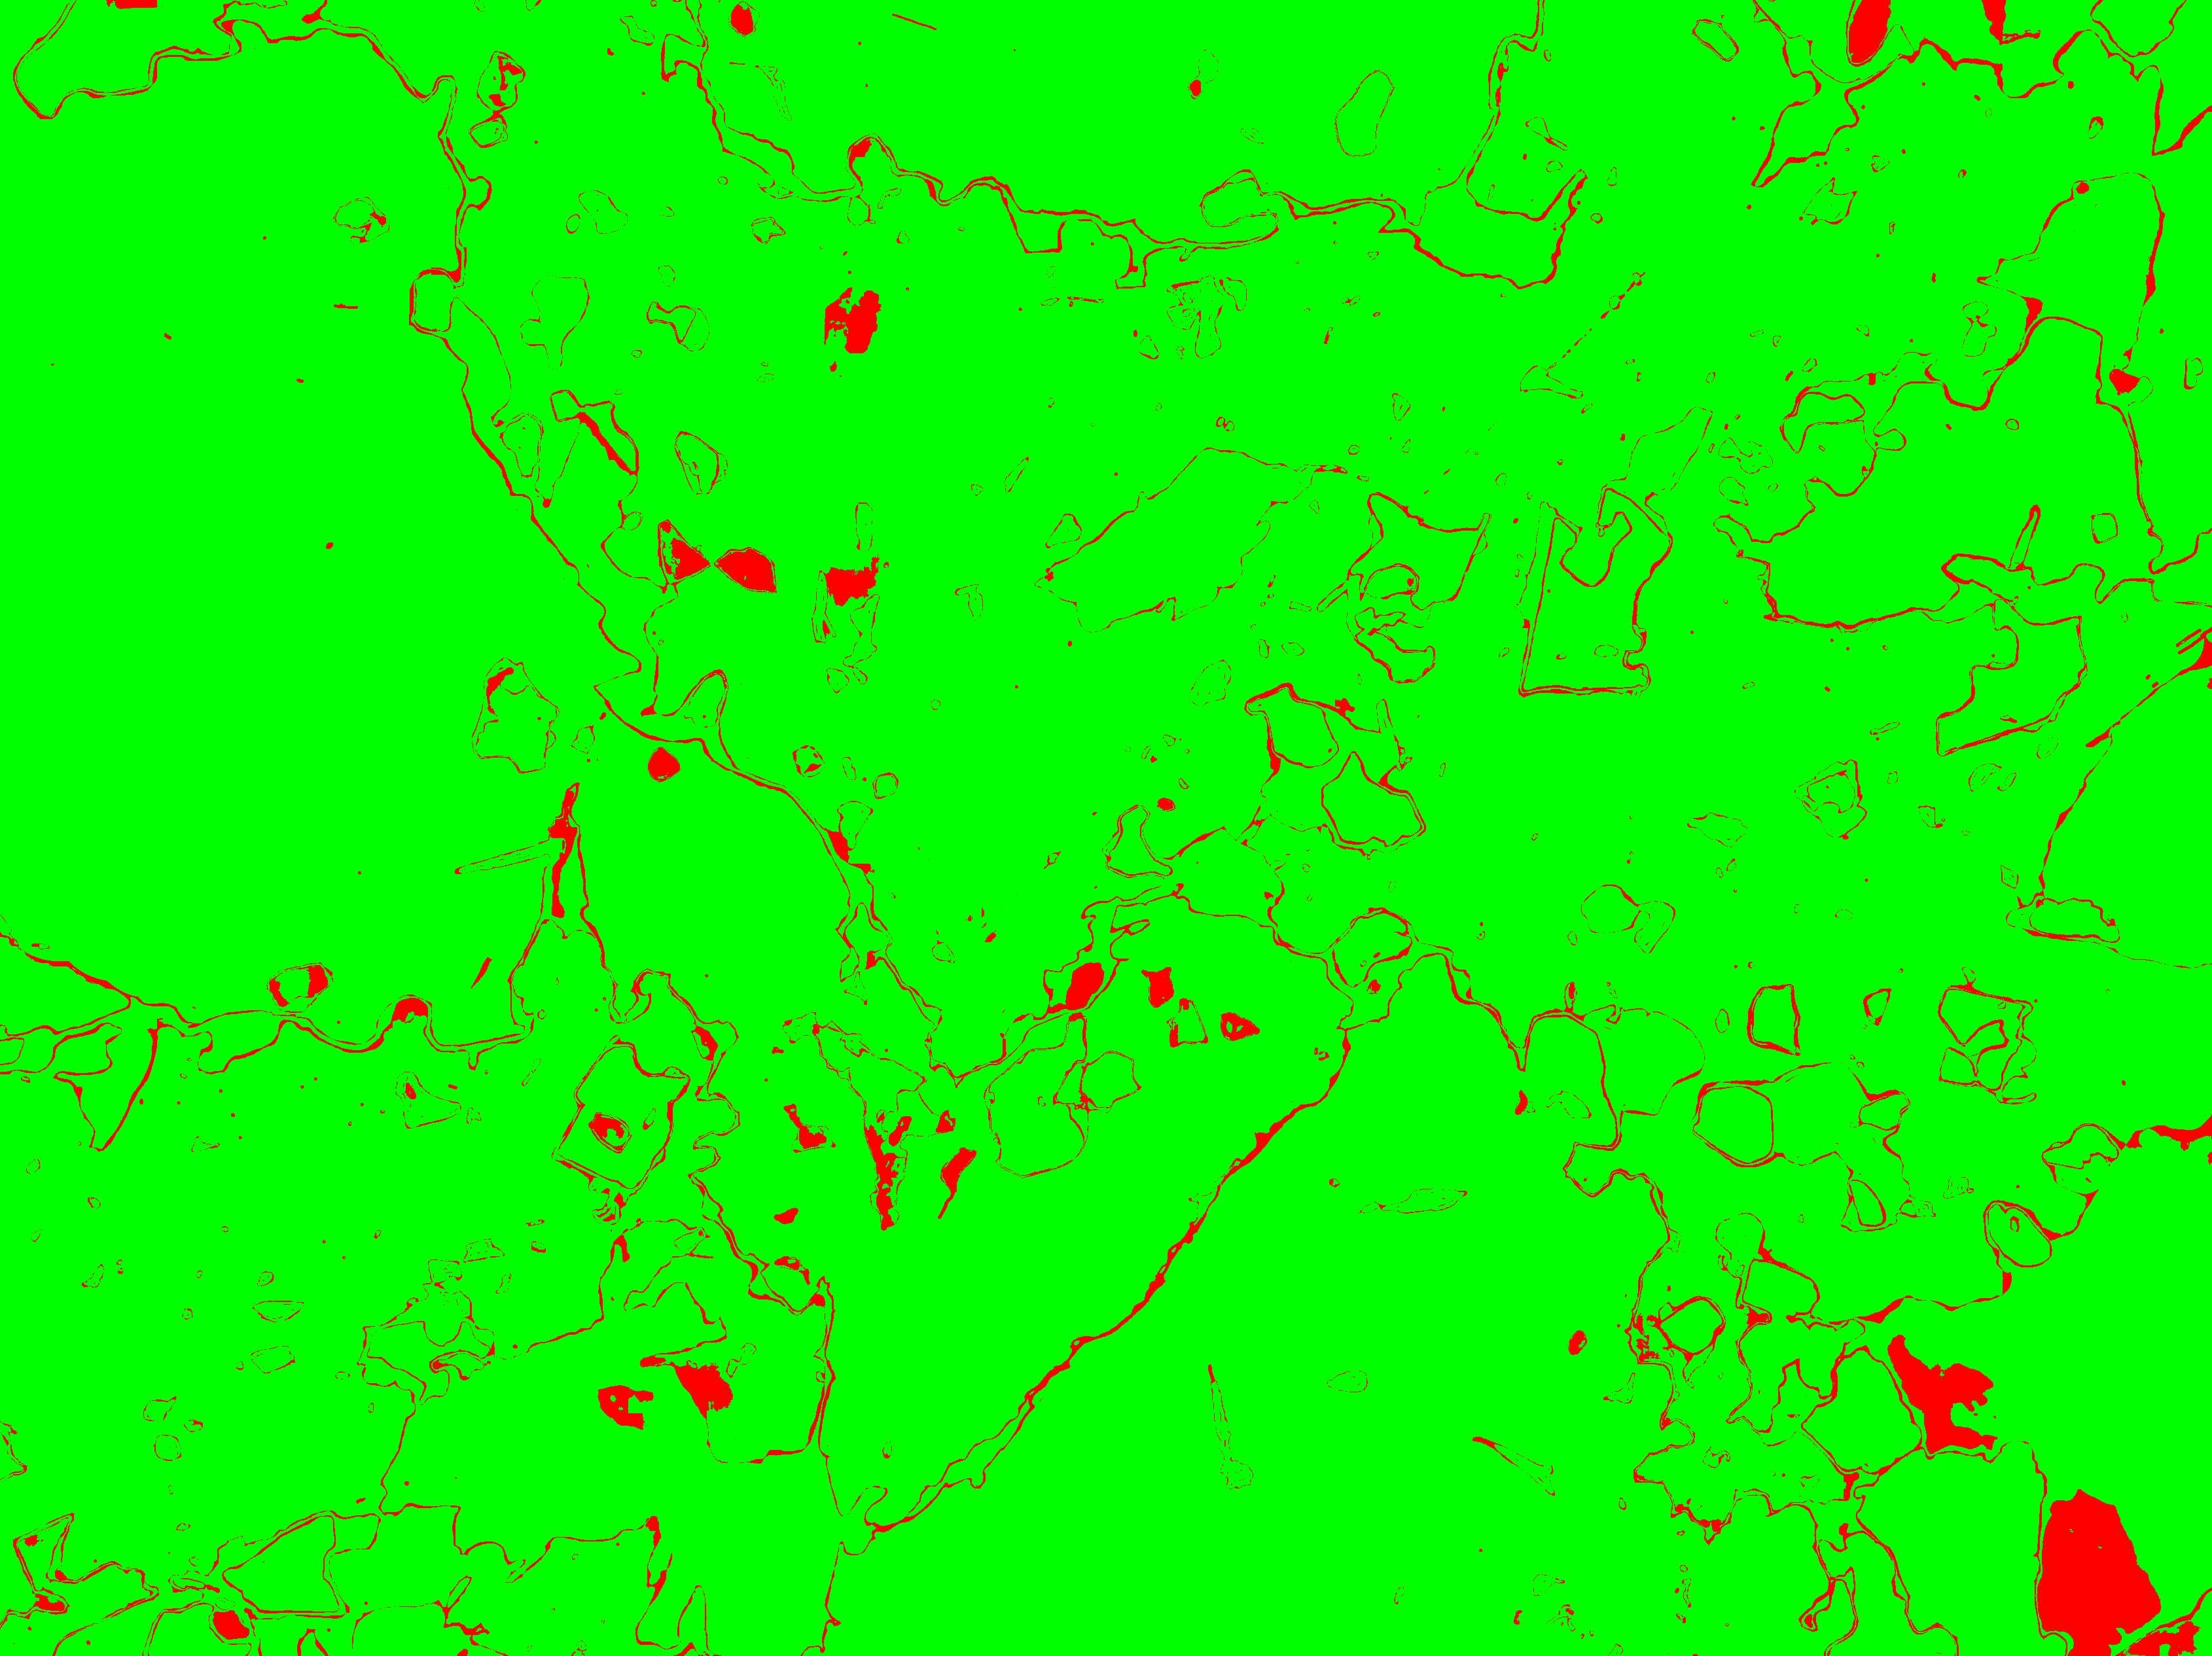
\includegraphics[width=.9\linewidth]{pics/image_5_error.jpg}
  \caption{Карта ошибок}
  \label{fig:sfig3_4}
\end{subfigure}%
\begin{subfigure}{.33\textwidth}
  \centering
  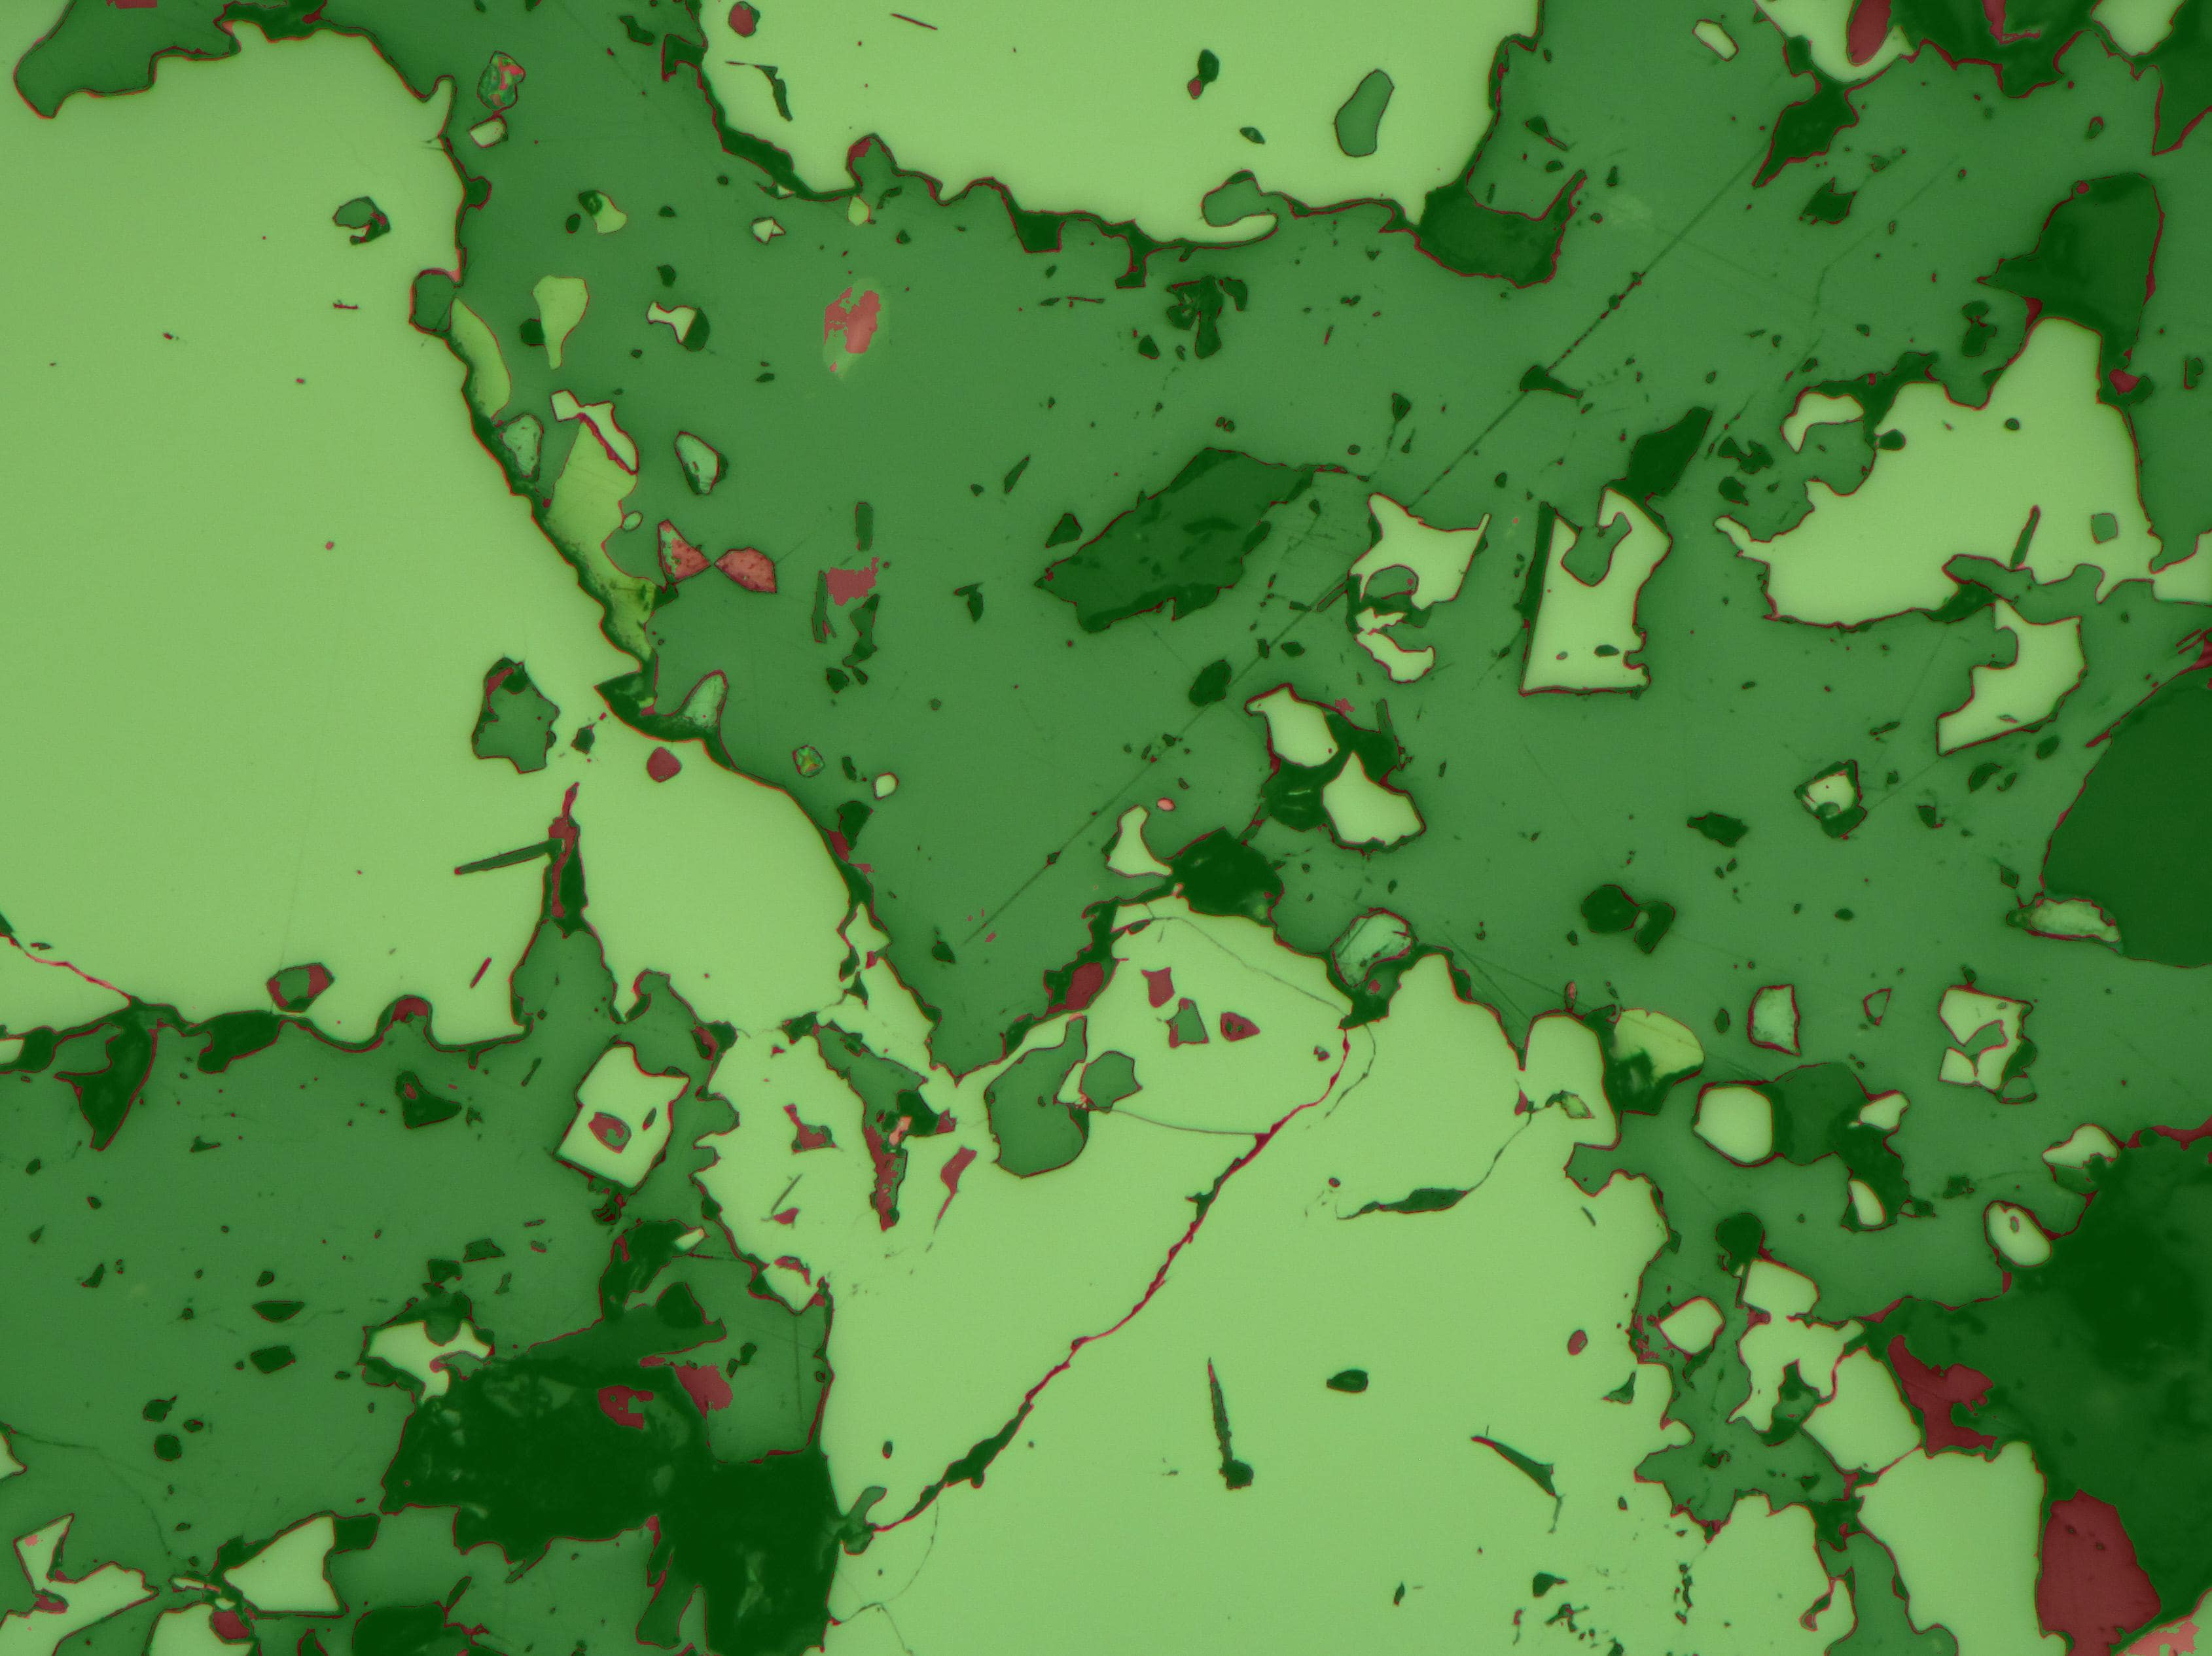
\includegraphics[width=.9\linewidth]{pics/image_5_overlay.jpg}
  \caption{Карта ошибок + исходное}
  \label{fig:sfig3_5}
\end{subfigure}
\caption{Тестовое изображение №3}
\label{fig:pred3}
\end{figure}

Тестовое изображение №3 было распознано правильно на 95.667\%, каждый из классов был распознан: \\
\begin{enumerate}[nosep]
    \item Background: 82.963\%
    \item Sh: 96.991\%
    \item Py/Mrc: 99.684\%
    \item Gl: 81.038\%
\end{enumerate}{}
Мера качества IoU показала следующие результаты:
\begin{enumerate}[nosep]
    \item Background: 0.73
    \item Sh: 0.92
    \item Py/Mrc: 0.97
    \item Gl: 0.59
\end{enumerate}{}

\newpage
Всего было протестировано 11 изображений. \\Средний процент правильной распознаваемости составил 92.4\%. Для каждого из классов:
\begin{enumerate}
    \item Background: 90.8\%
    \item Sh: 87.8\%
    \item Py/Mrc: 97.5\%
    \item Gl: 79.8\%
\end{enumerate}

\newpage
\section{Выводы}
В данной выпускной квалификационной работе был разработан и программно реализован на языке Python 3 с использованием фреймворков Tensorflow \cite{Tensorflow} и Keras \cite{Keras} метод автоматического анализа минерального состава руд по фотографиям аншлифов. Алгоритм показал высокую (выше 92\%) точность распознаваемости минералов и может быть использован в автоматизации разработки способов обогащения и в геолого-поисковых работах для выявления промышленного типа месторождения.
\par Также был разработан алгоритм балансировки данных для задачи семантической сегментации.


\newpage
\bibliography{bibliography}

\end{document}